\chapter{Image Transforms and Compression}

In Chapter~32 (Section~\ref{ch32:what-is-an-edge}) we used spatial convolution to isolate local features
like edges, corners, and blobs. Now we look at the image as an integrated whole and ask
the opposite question: how do we discard visual redundancy while preserving everything the
human eye actually notices?

A photograph straight off a camera sensor is heavily redundant. A single
twelve-megapixel image is roughly $12 \times 10^{6}$ pixels, each carrying three colour
channels of eight bits, which comes to about $36$ megabytes of raw data. Yet the JPEG
file you actually keep is often under two megabytes -- a twenty-to-one shrink -- and you
cannot see the difference. Something about images makes them \emph{compressible}: most
of the bits in the raw array are not telling you anything your eye would miss.

Most of the compression comes from \emph{changing coordinates}, not from clever bit-packing.
When we rotate an image block into an orthonormal basis aligned with spatial correlations,
its energy concentrates in a handful of large coefficients. We retain those key coefficients,
round the remainder toward zero, and store only what is visually essential. The
transform that JPEG uses -- the Discrete Cosine Transform -- is a close cousin of the
DFT, and everything we know about projection onto sinusoids carries straight over.

This chapter builds the DCT from the geometry up, shows \emph{why} a good transform
enables compression, walks JPEG end to end (block DCT, quantization, entropy coding),
and then says a word about the wavelet route that JPEG2000 takes. By the end you will
understand why a transform turns ``a lot of data'' into ``a little data plus error you
agreed not to care about,'' which is exactly the trade we will make later when our wrist
controller has to ship gesture features over a slow radio link.

\section{Why a transform enables compression}
\label{ch33:why-transform}

Start with the central picture. A small image patch -- say an $8\times 8$ block of
pixels -- is just a vector in a high-dimensional space, here $\R^{64}$. In the standard
pixel basis, each of the $64$ coordinates is one pixel's brightness, and for a natural
image \emph{all $64$ tend to be large and roughly equally important}. There is no obvious
way to drop any of them: every pixel matters about as much as every other.

Now rotate to a different orthonormal basis -- a different set of $64$ perpendicular
directions in the same space. The vector has not changed; only its coordinates have. If
we pick the basis well, the energy of natural image patches piles up into just a handful
of coordinates, leaving the rest near zero. \emph{Those} we can discard cheaply.

\begin{intuitionbox}
Transform compression is a change of viewpoint. Imagine a cloud of
data points that forms a long thin cigar tilted at $45^\circ$. In the original $x,y$
axes you need both coordinates to locate any point. Rotate the axes to lie \emph{along}
the cigar and one coordinate (the long one) carries almost all the variation while the
other (the thin one) is tiny. Keep the long coordinate, round the short one to zero, and
you have halved the storage while barely moving any point. The DCT does this in $64$
dimensions instead of $2$, and natural images really are ``cigar-shaped'': their energy
concentrates along a few smooth directions.
\end{intuitionbox}

\begin{figure}[H]
\centering
\begin{tikzpicture}
\begin{axis}[
  width=7.4cm, height=6.0cm,
  xlabel={$x$ (pixel A)}, ylabel={$y$ (pixel B)},
  xmin=-3.2, xmax=3.2, ymin=-3.2, ymax=3.2,
  axis lines=middle, xtick=\empty, ytick=\empty,
  enlargelimits=false,
]
\addplot[only marks, mark=*, mark size=1pt, sigblue]
  coordinates {(1.9,1.7)(-1.4,-1.6)(0.8,0.6)(-0.5,-0.7)(2.4,2.1)
  (-2.1,-1.9)(1.1,1.3)(-0.9,-0.6)(0.3,0.5)(-1.7,-1.4)(1.5,1.8)(-0.2,-0.3)};
\addplot[specred, very thick, -{Latex}] coordinates {(0,0)(2.3,2.1)};
\addplot[targetgreen, very thick, -{Latex}] coordinates {(0,0)(-0.6,0.65)};
\node[specred] at (axis cs:2.0,1.2) {\small long axis};
\node[targetgreen] at (axis cs:-1.7,1.1) {\small short axis};
\end{axis}
\end{tikzpicture}
\hfill
\begin{tikzpicture}
\begin{axis}[
  width=7.4cm, height=6.0cm,
  xlabel={$u$ (long axis)}, ylabel={$v$ (short axis)},
  xmin=-3.6, xmax=3.6, ymin=-3.6, ymax=3.6,
  axis lines=middle, xtick=\empty, ytick=\empty,
  enlargelimits=false,
]
\addplot[only marks, mark=*, mark size=1pt, sigblue]
  coordinates {(2.5,0.1)(-2.1,-0.1)(1.0,0.05)(-0.85,0.08)(3.2,-0.05)
  (-2.8,0.1)(1.7,-0.1)(-1.05,0.12)(0.55,-0.06)(-2.2,0.07)(2.3,-0.1)(-0.35,0.04)};
\draw[gray, dashed] (axis cs:-3.6,0.4) -- (axis cs:3.6,0.4);
\draw[gray, dashed] (axis cs:-3.6,-0.4) -- (axis cs:3.6,-0.4);
\end{axis}
\end{tikzpicture}
\caption{Two correlated pixels (left) live along a tilted cigar; both coordinates are
needed. After rotating the axes (right) almost all the spread is in $u$ while $v$ is
confined to a thin band near zero. Rounding $v$ to zero costs almost no error but halves
the data. A transform that does this for whole blocks is the basis of image
compression.}
\label{ch33:fig-cigar}
\end{figure}

\begin{whybox}
\textbf{Why does a transform let us drop coordinates at all?} Because energy is
conserved by an orthonormal change of basis (Parseval, which we proved for the DFT).
If $\vec{X} = \mat{T}\vec{x}$ with $\mat{T}$ orthonormal, then
$\norm{\vec{X}}^2 = \norm{\vec{x}}^2$: the total energy is the same in either basis.
What changes is the \emph{distribution} of that energy across coordinates. In the pixel
basis it is spread out; in a good transform basis it is concentrated. And if you
zero out a transform coefficient $X[k]$, the resulting reconstruction
error in the original domain is \emph{exactly} $\abs{X[k]}^2$ in energy, again by
Parseval. So discarding the smallest coefficients does the least damage, measured in the
same units the eye roughly cares about. The transform sorts the data into ``important''
and ``ignorable'' for you.
\end{whybox}

\textbf{A transform is a lossless rotation of coordinate axes; all loss in lossy compression
happens downstream, when we round or truncate the transformed coordinates.} The transform's
geometric role is to ensure that rounding discards minimal perceptual energy per stored bit.

\section{From DFT to DCT}
\label{ch33:dft-to-dct}

We already have a transform that compacts energy for smooth signals: the DFT. Why invent
a new one? The answer is about what happens at the \emph{edges} of a block.

Recall that the DFT treats its input as one period of a periodic signal. When you take
the DFT of an $8\times 8$ block, you are implicitly tiling the plane with copies of that
block. The right edge of one copy butts against the left edge of the next, and unless
those edges happen to match, you get a sharp jump at every seam. Sharp jumps are made of
high frequencies. So the DFT of an image block tends to have stubborn high-frequency
coefficients that are \emph{artifacts of the periodic wrap-around}, not real structure in
the image. They stay large, which ruins energy compaction and, worse, produces
ringing when you discard them.

\begin{intuitionbox}
The fix is easy to picture: before going periodic, \emph{mirror} the signal. Reflect the block about its right edge to make an even, symmetric signal of
double length, then make \emph{that} periodic. Now the seams match by construction --
the value on one side of a seam equals the value on the other -- so there is no
artificial jump. A signal that is mirror-symmetric has a Fourier representation made of
\emph{cosines only} (cosines are the even basis functions; sines, being odd, cancel).
That mirror-then-Fourier recipe \emph{is} the Discrete Cosine Transform.
\end{intuitionbox}

\begin{figure}[H]
\centering
\begin{tikzpicture}
\begin{axis}[
  width=12cm, height=4.6cm,
  xlabel={sample index (one block, then its periodic / mirrored extension)},
  ylabel={value}, ymin=-0.2, ymax=2.9, xmin=-0.5, xmax=23.5,
  xtick=\empty, axis lines=left, clip=false,
]
\addplot[ycomb, sigblue, thick, mark=*, mark size=1.2pt]
  coordinates {(0,0.4)(1,0.7)(2,1.0)(3,1.4)(4,1.7)(5,2.0)(6,2.2)(7,2.4)};
\addplot[ycomb, specred, thick, mark=o, mark size=1.2pt]
  coordinates {(8,0.4)(9,0.7)(10,1.0)(11,1.4)(12,1.7)(13,2.0)(14,2.2)(15,2.4)};
\draw[specred, dashed] (axis cs:7.5,-0.2) -- (axis cs:7.5,2.9);
\node[specred, fill=white, inner sep=2pt] at (axis cs:7.5,2.8) {\small DFT seam (jump)};
\addplot[ycomb, targetgreen, thick, mark=square*, mark size=1.0pt]
  coordinates {(16,2.4)(17,2.2)(18,2.0)(19,1.7)(20,1.4)(21,1.0)(22,0.7)(23,0.4)};
\draw[targetgreen, dashed] (axis cs:15.5,-0.2) -- (axis cs:15.5,2.9);
\node[targetgreen, fill=white, inner sep=2pt] at (axis cs:19.5,2.8) {\small DCT mirror (smooth)};
\end{axis}
\end{tikzpicture}
\caption{A ramp block (blue). The DFT periodically repeats it (red), creating a large
jump at every seam -- spurious high frequencies. The DCT first \emph{mirrors} the block
(green), so the extended signal is continuous across the seam and made of cosines only.
This is why the DCT compacts image energy better than the DFT.}
\label{ch33:fig-mirror}
\end{figure}

Let us write it down. For a length-$N$ signal $x[0],\dots,x[N-1]$, the (type-II)
\textbf{Discrete Cosine Transform} is
\begin{equation}
\label{ch33:dct-1d}
X[k] \;=\; \alpha_k \sum_{n=0}^{N-1} x[n]\,
\cos\!\left[\frac{\pi}{N}\Bigl(n+\tfrac{1}{2}\Bigr)k\right],
\qquad k = 0,\dots,N-1,
\end{equation}
with normalization $\alpha_0 = \sqrt{1/N}$ and $\alpha_k = \sqrt{2/N}$ for $k\ge 1$,
chosen so the transform is orthonormal. The inverse rebuilds $x$ from the same cosines:
\begin{equation}
\label{ch33:idct-1d}
x[n] \;=\; \sum_{k=0}^{N-1} \alpha_k\, X[k]\,
\cos\!\left[\frac{\pi}{N}\Bigl(n+\tfrac{1}{2}\Bigr)k\right].
\end{equation}
Read \eqref{ch33:dct-1d} exactly as you read the DFT: $X[k]$ is the inner product of the
signal with the $k$th basis cosine, i.e. \emph{how much of that cosine is in the signal}.
The half-sample shift $n+\tfrac12$ comes from the mirroring. The mirror sits halfway
between sample $-1$ and sample $0$, at $n=-\tfrac12$; measuring position from that plane
gives $n+\tfrac12$, so every basis cosine is even about the block's edge rather than about
a sample, which is what kills the seam.

\begin{focusbox}
\textbf{The DCT is real, orthonormal, and energy-preserving.} Unlike the DFT it maps
real inputs to real outputs (no complex arithmetic, no phase to store), its basis
vectors are mutually perpendicular unit vectors, and $\sum_k X[k]^2 = \sum_n x[n]^2$.
Coordinate $k=0$ is special: its cosine is constant, so $X[0]$ is proportional to the
block's \emph{average} brightness. It is called the DC coefficient, borrowing the
electrical term for a constant; all the rest are AC coefficients.
\end{focusbox}

\begin{connectionbox}
Everything here is the inner-product and orthogonal-basis machinery from linear
algebra (Chapter~42), reused directly. The DCT matrix $\mat{C}$ has orthonormal rows, so
$\mat{C}^{-1} = \mat{C}^{\!\top}$ -- inverting the transform is just transposing it. The
basis cosines are the eigenvectors of a particular symmetric tridiagonal matrix, which
is the underlying reason the DCT, and not some arbitrary cosine set, is the ``right'' one for
signals modelled as a smooth random process. We met the same eigenvector-of-a-shift
story when the DFT diagonalized circular convolution.
\end{connectionbox}

\subsection{The DCT basis functions, drawn}
\label{ch33:basis-drawn}

The eight one-dimensional DCT-II basis functions for $N=8$ are sampled cosines of
increasing frequency: a flat line ($k=0$), then a half-cycle, a full cycle, and so on up
to the fastest wiggle the block can hold. Figure \ref{ch33:fig-basis} draws the first
four. Reconstructing a block means scaling each of these by its coefficient $X[k]$ and
adding them up.

\begin{figure}[H]
\centering
\begin{tikzpicture}
\begin{axis}[
  width=10.6cm, height=5.2cm,
  xlabel={sample index $n$}, ylabel={amplitude},
  domain=0:7, samples=8, xmin=-0.3, xmax=7.3, ymin=-1.3, ymax=1.3,
  legend pos=outer north east, legend cell align=left,
  grid=both, grid style={gray!15}, axis lines=box,
  ytick={-1,0,1},
]
\addplot[sigblue, very thick, mark=*, mark size=1.2pt]
  {0.5}; \addlegendentry{$k=0$ (DC, flat)}
\addplot[specred, very thick, mark=*, mark size=1.2pt]
  {cos(deg(pi/8*(x+0.5)*1))}; \addlegendentry{$k=1$ (half cycle)}
\addplot[targetgreen, very thick, mark=*, mark size=1.2pt]
  {cos(deg(pi/8*(x+0.5)*2))}; \addlegendentry{$k=2$ (one cycle)}
\addplot[quotientorange, very thick, mark=*, mark size=1.2pt]
  {cos(deg(pi/8*(x+0.5)*3))}; \addlegendentry{$k=3$}
\end{axis}
\end{tikzpicture}
\caption{The first four DCT-II basis functions for a block of length $8$. Index $k=0$ is
constant (the average), and higher $k$ are progressively faster cosines. Any $8$-sample
signal is a weighted sum of these eight functions; the DCT computes the weights.}
\label{ch33:fig-basis}
\end{figure}

\begin{example}[A tiny DCT by hand]
\label{ch33:ex-tiny}
Take the smooth block $x = [10,10,10,10,12,12,12,12]$ -- flat, then a step up. Its
average is $11$, and the DC coefficient is $X[0] = \alpha_0\sum_n x[n] =
\sqrt{1/8}\cdot 88 \approx 31.1$. The signal is low-frequency, so the single step is
captured mainly by the lowest AC cosine. Computing the rest,
$X[1]\approx -2.56$, $X[2]=0$, $X[3]\approx 0.90$, $X[4]=0$, $X[5]\approx -0.60$,
$X[6]=0$, $X[7]\approx 0.51$. One coefficient, $X[1]$, carries essentially all the AC
energy; everything above it is several times smaller and the even-indexed AC terms vanish
outright. The zeros are symmetry, not luck: subtract the average and the block becomes
$[-1,-1,-1,-1,+1,+1,+1,+1]$, odd about its midpoint $n=3.5$, while every even-$k$ cosine is
even about that midpoint, so their inner product cancels pair by pair. Of the eight coefficients, only two matter: a small example of energy compaction.
\end{example}

\section{Energy compaction: the property that matters}
\label{ch33:energy-compaction}

We keep using the phrase ``energy compaction.'' Let us make it concrete and measurable,
because it is the single number that decides whether a transform is good for
compression.

Take many real image blocks, transform each, and look at where the energy lands across
coefficient indices. For natural images the DC and a few
lowest-frequency AC coefficients hold the overwhelming majority of the energy, and the
high-frequency coefficients are nearly zero almost all the time. Figure
\ref{ch33:fig-compaction} sketches the typical falloff.

\begin{figure}[H]
\centering
\begin{tikzpicture}
\begin{axis}[
  width=10.0cm, height=5.4cm,
  xlabel={coefficient index (low frequency $\rightarrow$ high frequency)},
  ylabel={average energy (log)},
  ymode=log, xmin=0, xmax=63, ymin=0.01, ymax=2000,
  grid=both, grid style={gray!15}, axis lines=box,
  legend pos=outer north east, legend cell align=left,
  legend style={fill=white, inner sep=4pt, draw=gray!40},
]
\addplot[specred, very thick, domain=0:63, samples=64] {1000*exp(-0.13*x)+0.05};
\addlegendentry{good transform (DCT)}
\addplot[gray, dashed, very thick, domain=0:63, samples=64] {30};
\addlegendentry{pixel basis (flat)}
\end{axis}
\end{tikzpicture}
\caption{Average energy per coefficient for a $64$-coefficient block. In the pixel basis
(gray) energy is flat -- every pixel matters equally. After the DCT (red) energy falls
off steeply: the first handful of coefficients dominate, and the high-frequency tail is
orders of magnitude smaller. Compression keeps the head of this curve and discards the
tail.}
\label{ch33:fig-compaction}
\end{figure}

\begin{happeningbox}
The reason is that natural images are \emph{spatially correlated}:
neighbouring pixels are almost always similar. Correlation in the pixel domain becomes
\emph{concentration} in the transform domain, and this holds in general. The more
predictable a pixel is from its neighbours, the more the transform can pack into a few
coefficients. Pure random noise, where no pixel predicts any other, has no correlation,
so it does \emph{not} compact -- its energy stays flat in every orthonormal basis. That
is precisely why noise is incompressible and why JPEG handles a clean portrait far
better than a photo of static.
\end{happeningbox}

\begin{historybox}
\textbf{Nasir Ahmed, the National Science Foundation Rejection, and the DCT (1974)}

In the early 1970s, digital imaging was severely limited by cost. A single uncompressed $512\times 512$ pixel black-and-white image consumed a quarter of a megabyte of memory at a time when magnetic-core memory cost thousands of dollars per megabyte and phone-line modems ran at $300$ baud. 

Information theory had already discovered the mathematically optimal transform for energy compaction: the \textbf{Karhunen--Lo\`eve Transform} (KLT), derived by Kari Karhunen (1947) and Michel Lo\`eve (1948). The KLT projects data onto the eigenvectors of the signal's empirical covariance matrix $\mat{R}_{\vec{x}\vec{x}} = \E[\vec{x}\vec{x}^\top]$. By construction, the KLT perfectly diagonalizes the covariance, completely decorrelating the coefficients and packing the maximum possible variance into the first few terms.

For practical engineering, however, the KLT was impractical. It was strictly \emph{data-dependent}: to compress an image, the transmitter had to estimate the sample covariance matrix for each image block, compute its full eigendecomposition (an $O(N^3)$ matrix diagonalization on hardware like a DEC PDP-11 with a 16-bit processor and a few kilobytes of RAM), and then transmit the custom eigenvectors alongside the compressed payload.

In 1972, Nasir Ahmed at Kansas State University realized that images share a predictable statistical structure: neighboring pixels are strongly correlated, behaving like a stationary first-order Gauss--Markov process with adjacent correlation coefficient $\rho \approx 0.95$. Ahmed hypothesized that a fixed, data-independent orthogonal transform constructed purely from sampled cosines could mimic the KLT eigenvectors.

When Ahmed submitted a grant proposal to the U.S. National Science Foundation (NSF) proposing to investigate this cosine transform, it was rejected. Reviewers argued that Fourier analysis (the DFT) was already well understood and asking why anyone would need another cosine transform when complex sinusoids already spanned the space.

Ahmed persisted without funding. Working with T.~Natarajan and K.~R.~Rao, he proved in 1974 that as the Markov correlation parameter $\rho \to 1$, the eigenvectors of the Toeplitz covariance matrix (whose diagonals are constant, reflecting stationary neighbor correlations) analytically converge to the exact Type-II Discrete Cosine Transform basis vectors. The DCT is therefore the asymptotic limit of the optimal KLT, not just an empirical heuristic. Because the DCT basis is fixed, it can be computed with fast butterfly algorithms ($O(N \log N)$) without computing covariances or transmitting eigenvectors.

When the Joint Photographic Experts Group standardized JPEG in 1992, Ahmed's DCT was chosen as its core transform, soon powering digital video from MPEG-2 through modern codecs. What remains challenging is the rigid $8\times 8$ block boundary, which creates visible tiling seams at very low bitrates --- motivating multi-scale wavelets and modern neural compression.
\end{historybox}

\begin{trapbox}
\textbf{Why the Naive Idea Fails: Why not the standard DFT?}
A natural first idea is: ``We already have the Fast Fourier Transform (FFT); why not apply the 2D DFT to each image block?''

The failure is rooted in boundary conditions. The DFT implicitly assumes that each $8\times 8$ block repeats \emph{periodically} across all of $\R^2$. If the top-left pixel is bright ($240$) and the top-right pixel is dark ($30$), wrapping around creates a steep cliff --- an artificial jump discontinuity of $210$ intensity levels right at the block boundary. Because sharp cliffs contain infinite high frequencies (the Gibbs phenomenon), the 2D DFT must spend dozens of high-frequency complex exponential coefficients just to cancel the artificial edge discontinuity that only existed because of the periodic wrapping.

The DCT solves this by implicitly performing an \emph{even symmetric reflection} at every block boundary: $x[-1] = x[0]$ and $x[N] = x[N-1]$. The mirrored block has continuous, smoothly rolling boundaries at every seam. The artificial cliff vanishes, allowing the DCT to concentrate nearly all image energy into the lowest 3 or 4 coefficients, while the DFT spreads energy across the entire spectrum.
\end{trapbox}

\section{The 2D DCT}
\label{ch33:2d-dct}

Images are two-dimensional, so we need a 2D transform. The trick is the same
separability we used for the 2D Fourier transform: a 2D DCT is just a 1D DCT applied to
every row, then a 1D DCT applied to every column of the result (or vice versa -- the
order does not matter). Formally, for an $N\times N$ block $x[m,n]$,
\begin{equation}
\label{ch33:dct-2d}
X[k,\ell] \;=\; \alpha_k\,\alpha_\ell
\sum_{m=0}^{N-1}\sum_{n=0}^{N-1} x[m,n]\,
\cos\!\Bigl[\tfrac{\pi}{N}(m+\tfrac12)k\Bigr]
\cos\!\Bigl[\tfrac{\pi}{N}(n+\tfrac12)\ell\Bigr].
\end{equation}
Each 2D basis function is the outer product of a vertical cosine (in the row index $m$,
frequency $k$) and a horizontal cosine (in the column index $n$, frequency $\ell$), giving
a little checkerboard-like pattern. For an $8\times 8$ block there are $64$ such patterns.
Figure~\ref{ch33:fig-2dbasis} arranges them with horizontal frequency $u=\ell$ across and
vertical frequency $v=k$ down. The top-left pattern ($k=\ell=0$) is flat -- pure average
brightness. Move right and the brightness oscillates faster as you cross the columns, so
the pattern gains finer \emph{vertical} bars; move down and it oscillates faster down the
rows, so it gains finer \emph{horizontal} bars; the bottom-right pattern is the finest
checkerboard the block can represent.

\begin{figure}[H]
\centering
\begin{tikzpicture}[scale=0.175]
% Frequency rulers
\node[font=\small\bfseries] at (37, 8.0) {Horizontal spatial frequency $u \rightarrow$};
\node[rotate=90, font=\small\bfseries] at (-6.8, -37) {Vertical spatial frequency $v \rightarrow$};
\node[font=\footnotesize] at (4.0, 1.5) {$u=0$};
\node[font=\footnotesize] at (13.5, 1.5) {$u=1$};
\node[font=\footnotesize] at (23.0, 1.5) {$u=2$};
\node[font=\footnotesize] at (32.5, 1.5) {$u=3$};
\node[font=\footnotesize] at (42.0, 1.5) {$u=4$};
\node[font=\footnotesize] at (51.5, 1.5) {$u=5$};
\node[font=\footnotesize] at (61.0, 1.5) {$u=6$};
\node[font=\footnotesize] at (70.5, 1.5) {$u=7$};
\node[font=\footnotesize] at (-2.5, -4.0) {$v=0$};
\node[font=\footnotesize] at (-2.5, -13.5) {$v=1$};
\node[font=\footnotesize] at (-2.5, -23.0) {$v=2$};
\node[font=\footnotesize] at (-2.5, -32.5) {$v=3$};
\node[font=\footnotesize] at (-2.5, -42.0) {$v=4$};
\node[font=\footnotesize] at (-2.5, -51.5) {$v=5$};
\node[font=\footnotesize] at (-2.5, -61.0) {$v=6$};
\node[font=\footnotesize] at (-2.5, -70.5) {$v=7$};
\begin{scope}[shift={(0.0, 0.0)}]
  \fill[black!100] (0,0) rectangle (1,-1);
  \fill[black!100] (1,0) rectangle (2,-1);
  \fill[black!100] (2,0) rectangle (3,-1);
  \fill[black!100] (3,0) rectangle (4,-1);
  \fill[black!100] (4,0) rectangle (5,-1);
  \fill[black!100] (5,0) rectangle (6,-1);
  \fill[black!100] (6,0) rectangle (7,-1);
  \fill[black!100] (7,0) rectangle (8,-1);
  \fill[black!100] (0,-1) rectangle (1,-2);
  \fill[black!100] (1,-1) rectangle (2,-2);
  \fill[black!100] (2,-1) rectangle (3,-2);
  \fill[black!100] (3,-1) rectangle (4,-2);
  \fill[black!100] (4,-1) rectangle (5,-2);
  \fill[black!100] (5,-1) rectangle (6,-2);
  \fill[black!100] (6,-1) rectangle (7,-2);
  \fill[black!100] (7,-1) rectangle (8,-2);
  \fill[black!100] (0,-2) rectangle (1,-3);
  \fill[black!100] (1,-2) rectangle (2,-3);
  \fill[black!100] (2,-2) rectangle (3,-3);
  \fill[black!100] (3,-2) rectangle (4,-3);
  \fill[black!100] (4,-2) rectangle (5,-3);
  \fill[black!100] (5,-2) rectangle (6,-3);
  \fill[black!100] (6,-2) rectangle (7,-3);
  \fill[black!100] (7,-2) rectangle (8,-3);
  \fill[black!100] (0,-3) rectangle (1,-4);
  \fill[black!100] (1,-3) rectangle (2,-4);
  \fill[black!100] (2,-3) rectangle (3,-4);
  \fill[black!100] (3,-3) rectangle (4,-4);
  \fill[black!100] (4,-3) rectangle (5,-4);
  \fill[black!100] (5,-3) rectangle (6,-4);
  \fill[black!100] (6,-3) rectangle (7,-4);
  \fill[black!100] (7,-3) rectangle (8,-4);
  \fill[black!100] (0,-4) rectangle (1,-5);
  \fill[black!100] (1,-4) rectangle (2,-5);
  \fill[black!100] (2,-4) rectangle (3,-5);
  \fill[black!100] (3,-4) rectangle (4,-5);
  \fill[black!100] (4,-4) rectangle (5,-5);
  \fill[black!100] (5,-4) rectangle (6,-5);
  \fill[black!100] (6,-4) rectangle (7,-5);
  \fill[black!100] (7,-4) rectangle (8,-5);
  \fill[black!100] (0,-5) rectangle (1,-6);
  \fill[black!100] (1,-5) rectangle (2,-6);
  \fill[black!100] (2,-5) rectangle (3,-6);
  \fill[black!100] (3,-5) rectangle (4,-6);
  \fill[black!100] (4,-5) rectangle (5,-6);
  \fill[black!100] (5,-5) rectangle (6,-6);
  \fill[black!100] (6,-5) rectangle (7,-6);
  \fill[black!100] (7,-5) rectangle (8,-6);
  \fill[black!100] (0,-6) rectangle (1,-7);
  \fill[black!100] (1,-6) rectangle (2,-7);
  \fill[black!100] (2,-6) rectangle (3,-7);
  \fill[black!100] (3,-6) rectangle (4,-7);
  \fill[black!100] (4,-6) rectangle (5,-7);
  \fill[black!100] (5,-6) rectangle (6,-7);
  \fill[black!100] (6,-6) rectangle (7,-7);
  \fill[black!100] (7,-6) rectangle (8,-7);
  \fill[black!100] (0,-7) rectangle (1,-8);
  \fill[black!100] (1,-7) rectangle (2,-8);
  \fill[black!100] (2,-7) rectangle (3,-8);
  \fill[black!100] (3,-7) rectangle (4,-8);
  \fill[black!100] (4,-7) rectangle (5,-8);
  \fill[black!100] (5,-7) rectangle (6,-8);
  \fill[black!100] (6,-7) rectangle (7,-8);
  \fill[black!100] (7,-7) rectangle (8,-8);
  \draw[gray!70, line width=0.4pt] (0,0) rectangle (8,-8);
\end{scope}
\begin{scope}[shift={(9.5, 0.0)}]
  \fill[black!99] (0,0) rectangle (1,-1);
  \fill[black!92] (1,0) rectangle (2,-1);
  \fill[black!78] (2,0) rectangle (3,-1);
  \fill[black!60] (3,0) rectangle (4,-1);
  \fill[black!40] (4,0) rectangle (5,-1);
  \fill[black!22] (5,0) rectangle (6,-1);
  \fill[black!8] (6,0) rectangle (7,-1);
  \fill[black!1] (7,0) rectangle (8,-1);
  \fill[black!99] (0,-1) rectangle (1,-2);
  \fill[black!92] (1,-1) rectangle (2,-2);
  \fill[black!78] (2,-1) rectangle (3,-2);
  \fill[black!60] (3,-1) rectangle (4,-2);
  \fill[black!40] (4,-1) rectangle (5,-2);
  \fill[black!22] (5,-1) rectangle (6,-2);
  \fill[black!8] (6,-1) rectangle (7,-2);
  \fill[black!1] (7,-1) rectangle (8,-2);
  \fill[black!99] (0,-2) rectangle (1,-3);
  \fill[black!92] (1,-2) rectangle (2,-3);
  \fill[black!78] (2,-2) rectangle (3,-3);
  \fill[black!60] (3,-2) rectangle (4,-3);
  \fill[black!40] (4,-2) rectangle (5,-3);
  \fill[black!22] (5,-2) rectangle (6,-3);
  \fill[black!8] (6,-2) rectangle (7,-3);
  \fill[black!1] (7,-2) rectangle (8,-3);
  \fill[black!99] (0,-3) rectangle (1,-4);
  \fill[black!92] (1,-3) rectangle (2,-4);
  \fill[black!78] (2,-3) rectangle (3,-4);
  \fill[black!60] (3,-3) rectangle (4,-4);
  \fill[black!40] (4,-3) rectangle (5,-4);
  \fill[black!22] (5,-3) rectangle (6,-4);
  \fill[black!8] (6,-3) rectangle (7,-4);
  \fill[black!1] (7,-3) rectangle (8,-4);
  \fill[black!99] (0,-4) rectangle (1,-5);
  \fill[black!92] (1,-4) rectangle (2,-5);
  \fill[black!78] (2,-4) rectangle (3,-5);
  \fill[black!60] (3,-4) rectangle (4,-5);
  \fill[black!40] (4,-4) rectangle (5,-5);
  \fill[black!22] (5,-4) rectangle (6,-5);
  \fill[black!8] (6,-4) rectangle (7,-5);
  \fill[black!1] (7,-4) rectangle (8,-5);
  \fill[black!99] (0,-5) rectangle (1,-6);
  \fill[black!92] (1,-5) rectangle (2,-6);
  \fill[black!78] (2,-5) rectangle (3,-6);
  \fill[black!60] (3,-5) rectangle (4,-6);
  \fill[black!40] (4,-5) rectangle (5,-6);
  \fill[black!22] (5,-5) rectangle (6,-6);
  \fill[black!8] (6,-5) rectangle (7,-6);
  \fill[black!1] (7,-5) rectangle (8,-6);
  \fill[black!99] (0,-6) rectangle (1,-7);
  \fill[black!92] (1,-6) rectangle (2,-7);
  \fill[black!78] (2,-6) rectangle (3,-7);
  \fill[black!60] (3,-6) rectangle (4,-7);
  \fill[black!40] (4,-6) rectangle (5,-7);
  \fill[black!22] (5,-6) rectangle (6,-7);
  \fill[black!8] (6,-6) rectangle (7,-7);
  \fill[black!1] (7,-6) rectangle (8,-7);
  \fill[black!99] (0,-7) rectangle (1,-8);
  \fill[black!92] (1,-7) rectangle (2,-8);
  \fill[black!78] (2,-7) rectangle (3,-8);
  \fill[black!60] (3,-7) rectangle (4,-8);
  \fill[black!40] (4,-7) rectangle (5,-8);
  \fill[black!22] (5,-7) rectangle (6,-8);
  \fill[black!8] (6,-7) rectangle (7,-8);
  \fill[black!1] (7,-7) rectangle (8,-8);
  \draw[gray!70, line width=0.4pt] (0,0) rectangle (8,-8);
\end{scope}
\begin{scope}[shift={(19.0, 0.0)}]
  \fill[black!96] (0,0) rectangle (1,-1);
  \fill[black!69] (1,0) rectangle (2,-1);
  \fill[black!31] (2,0) rectangle (3,-1);
  \fill[black!4] (3,0) rectangle (4,-1);
  \fill[black!4] (4,0) rectangle (5,-1);
  \fill[black!31] (5,0) rectangle (6,-1);
  \fill[black!69] (6,0) rectangle (7,-1);
  \fill[black!96] (7,0) rectangle (8,-1);
  \fill[black!96] (0,-1) rectangle (1,-2);
  \fill[black!69] (1,-1) rectangle (2,-2);
  \fill[black!31] (2,-1) rectangle (3,-2);
  \fill[black!4] (3,-1) rectangle (4,-2);
  \fill[black!4] (4,-1) rectangle (5,-2);
  \fill[black!31] (5,-1) rectangle (6,-2);
  \fill[black!69] (6,-1) rectangle (7,-2);
  \fill[black!96] (7,-1) rectangle (8,-2);
  \fill[black!96] (0,-2) rectangle (1,-3);
  \fill[black!69] (1,-2) rectangle (2,-3);
  \fill[black!31] (2,-2) rectangle (3,-3);
  \fill[black!4] (3,-2) rectangle (4,-3);
  \fill[black!4] (4,-2) rectangle (5,-3);
  \fill[black!31] (5,-2) rectangle (6,-3);
  \fill[black!69] (6,-2) rectangle (7,-3);
  \fill[black!96] (7,-2) rectangle (8,-3);
  \fill[black!96] (0,-3) rectangle (1,-4);
  \fill[black!69] (1,-3) rectangle (2,-4);
  \fill[black!31] (2,-3) rectangle (3,-4);
  \fill[black!4] (3,-3) rectangle (4,-4);
  \fill[black!4] (4,-3) rectangle (5,-4);
  \fill[black!31] (5,-3) rectangle (6,-4);
  \fill[black!69] (6,-3) rectangle (7,-4);
  \fill[black!96] (7,-3) rectangle (8,-4);
  \fill[black!96] (0,-4) rectangle (1,-5);
  \fill[black!69] (1,-4) rectangle (2,-5);
  \fill[black!31] (2,-4) rectangle (3,-5);
  \fill[black!4] (3,-4) rectangle (4,-5);
  \fill[black!4] (4,-4) rectangle (5,-5);
  \fill[black!31] (5,-4) rectangle (6,-5);
  \fill[black!69] (6,-4) rectangle (7,-5);
  \fill[black!96] (7,-4) rectangle (8,-5);
  \fill[black!96] (0,-5) rectangle (1,-6);
  \fill[black!69] (1,-5) rectangle (2,-6);
  \fill[black!31] (2,-5) rectangle (3,-6);
  \fill[black!4] (3,-5) rectangle (4,-6);
  \fill[black!4] (4,-5) rectangle (5,-6);
  \fill[black!31] (5,-5) rectangle (6,-6);
  \fill[black!69] (6,-5) rectangle (7,-6);
  \fill[black!96] (7,-5) rectangle (8,-6);
  \fill[black!96] (0,-6) rectangle (1,-7);
  \fill[black!69] (1,-6) rectangle (2,-7);
  \fill[black!31] (2,-6) rectangle (3,-7);
  \fill[black!4] (3,-6) rectangle (4,-7);
  \fill[black!4] (4,-6) rectangle (5,-7);
  \fill[black!31] (5,-6) rectangle (6,-7);
  \fill[black!69] (6,-6) rectangle (7,-7);
  \fill[black!96] (7,-6) rectangle (8,-7);
  \fill[black!96] (0,-7) rectangle (1,-8);
  \fill[black!69] (1,-7) rectangle (2,-8);
  \fill[black!31] (2,-7) rectangle (3,-8);
  \fill[black!4] (3,-7) rectangle (4,-8);
  \fill[black!4] (4,-7) rectangle (5,-8);
  \fill[black!31] (5,-7) rectangle (6,-8);
  \fill[black!69] (6,-7) rectangle (7,-8);
  \fill[black!96] (7,-7) rectangle (8,-8);
  \draw[gray!70, line width=0.4pt] (0,0) rectangle (8,-8);
\end{scope}
\begin{scope}[shift={(28.5, 0.0)}]
  \fill[black!92] (0,0) rectangle (1,-1);
  \fill[black!40] (1,0) rectangle (2,-1);
  \fill[black!1] (2,0) rectangle (3,-1);
  \fill[black!22] (3,0) rectangle (4,-1);
  \fill[black!78] (4,0) rectangle (5,-1);
  \fill[black!99] (5,0) rectangle (6,-1);
  \fill[black!60] (6,0) rectangle (7,-1);
  \fill[black!8] (7,0) rectangle (8,-1);
  \fill[black!92] (0,-1) rectangle (1,-2);
  \fill[black!40] (1,-1) rectangle (2,-2);
  \fill[black!1] (2,-1) rectangle (3,-2);
  \fill[black!22] (3,-1) rectangle (4,-2);
  \fill[black!78] (4,-1) rectangle (5,-2);
  \fill[black!99] (5,-1) rectangle (6,-2);
  \fill[black!60] (6,-1) rectangle (7,-2);
  \fill[black!8] (7,-1) rectangle (8,-2);
  \fill[black!92] (0,-2) rectangle (1,-3);
  \fill[black!40] (1,-2) rectangle (2,-3);
  \fill[black!1] (2,-2) rectangle (3,-3);
  \fill[black!22] (3,-2) rectangle (4,-3);
  \fill[black!78] (4,-2) rectangle (5,-3);
  \fill[black!99] (5,-2) rectangle (6,-3);
  \fill[black!60] (6,-2) rectangle (7,-3);
  \fill[black!8] (7,-2) rectangle (8,-3);
  \fill[black!92] (0,-3) rectangle (1,-4);
  \fill[black!40] (1,-3) rectangle (2,-4);
  \fill[black!1] (2,-3) rectangle (3,-4);
  \fill[black!22] (3,-3) rectangle (4,-4);
  \fill[black!78] (4,-3) rectangle (5,-4);
  \fill[black!99] (5,-3) rectangle (6,-4);
  \fill[black!60] (6,-3) rectangle (7,-4);
  \fill[black!8] (7,-3) rectangle (8,-4);
  \fill[black!92] (0,-4) rectangle (1,-5);
  \fill[black!40] (1,-4) rectangle (2,-5);
  \fill[black!1] (2,-4) rectangle (3,-5);
  \fill[black!22] (3,-4) rectangle (4,-5);
  \fill[black!78] (4,-4) rectangle (5,-5);
  \fill[black!99] (5,-4) rectangle (6,-5);
  \fill[black!60] (6,-4) rectangle (7,-5);
  \fill[black!8] (7,-4) rectangle (8,-5);
  \fill[black!92] (0,-5) rectangle (1,-6);
  \fill[black!40] (1,-5) rectangle (2,-6);
  \fill[black!1] (2,-5) rectangle (3,-6);
  \fill[black!22] (3,-5) rectangle (4,-6);
  \fill[black!78] (4,-5) rectangle (5,-6);
  \fill[black!99] (5,-5) rectangle (6,-6);
  \fill[black!60] (6,-5) rectangle (7,-6);
  \fill[black!8] (7,-5) rectangle (8,-6);
  \fill[black!92] (0,-6) rectangle (1,-7);
  \fill[black!40] (1,-6) rectangle (2,-7);
  \fill[black!1] (2,-6) rectangle (3,-7);
  \fill[black!22] (3,-6) rectangle (4,-7);
  \fill[black!78] (4,-6) rectangle (5,-7);
  \fill[black!99] (5,-6) rectangle (6,-7);
  \fill[black!60] (6,-6) rectangle (7,-7);
  \fill[black!8] (7,-6) rectangle (8,-7);
  \fill[black!92] (0,-7) rectangle (1,-8);
  \fill[black!40] (1,-7) rectangle (2,-8);
  \fill[black!1] (2,-7) rectangle (3,-8);
  \fill[black!22] (3,-7) rectangle (4,-8);
  \fill[black!78] (4,-7) rectangle (5,-8);
  \fill[black!99] (5,-7) rectangle (6,-8);
  \fill[black!60] (6,-7) rectangle (7,-8);
  \fill[black!8] (7,-7) rectangle (8,-8);
  \draw[gray!70, line width=0.4pt] (0,0) rectangle (8,-8);
\end{scope}
\begin{scope}[shift={(38.0, 0.0)}]
  \fill[black!85] (0,0) rectangle (1,-1);
  \fill[black!15] (1,0) rectangle (2,-1);
  \fill[black!15] (2,0) rectangle (3,-1);
  \fill[black!85] (3,0) rectangle (4,-1);
  \fill[black!85] (4,0) rectangle (5,-1);
  \fill[black!15] (5,0) rectangle (6,-1);
  \fill[black!15] (6,0) rectangle (7,-1);
  \fill[black!85] (7,0) rectangle (8,-1);
  \fill[black!85] (0,-1) rectangle (1,-2);
  \fill[black!15] (1,-1) rectangle (2,-2);
  \fill[black!15] (2,-1) rectangle (3,-2);
  \fill[black!85] (3,-1) rectangle (4,-2);
  \fill[black!85] (4,-1) rectangle (5,-2);
  \fill[black!15] (5,-1) rectangle (6,-2);
  \fill[black!15] (6,-1) rectangle (7,-2);
  \fill[black!85] (7,-1) rectangle (8,-2);
  \fill[black!85] (0,-2) rectangle (1,-3);
  \fill[black!15] (1,-2) rectangle (2,-3);
  \fill[black!15] (2,-2) rectangle (3,-3);
  \fill[black!85] (3,-2) rectangle (4,-3);
  \fill[black!85] (4,-2) rectangle (5,-3);
  \fill[black!15] (5,-2) rectangle (6,-3);
  \fill[black!15] (6,-2) rectangle (7,-3);
  \fill[black!85] (7,-2) rectangle (8,-3);
  \fill[black!85] (0,-3) rectangle (1,-4);
  \fill[black!15] (1,-3) rectangle (2,-4);
  \fill[black!15] (2,-3) rectangle (3,-4);
  \fill[black!85] (3,-3) rectangle (4,-4);
  \fill[black!85] (4,-3) rectangle (5,-4);
  \fill[black!15] (5,-3) rectangle (6,-4);
  \fill[black!15] (6,-3) rectangle (7,-4);
  \fill[black!85] (7,-3) rectangle (8,-4);
  \fill[black!85] (0,-4) rectangle (1,-5);
  \fill[black!15] (1,-4) rectangle (2,-5);
  \fill[black!15] (2,-4) rectangle (3,-5);
  \fill[black!85] (3,-4) rectangle (4,-5);
  \fill[black!85] (4,-4) rectangle (5,-5);
  \fill[black!15] (5,-4) rectangle (6,-5);
  \fill[black!15] (6,-4) rectangle (7,-5);
  \fill[black!85] (7,-4) rectangle (8,-5);
  \fill[black!85] (0,-5) rectangle (1,-6);
  \fill[black!15] (1,-5) rectangle (2,-6);
  \fill[black!15] (2,-5) rectangle (3,-6);
  \fill[black!85] (3,-5) rectangle (4,-6);
  \fill[black!85] (4,-5) rectangle (5,-6);
  \fill[black!15] (5,-5) rectangle (6,-6);
  \fill[black!15] (6,-5) rectangle (7,-6);
  \fill[black!85] (7,-5) rectangle (8,-6);
  \fill[black!85] (0,-6) rectangle (1,-7);
  \fill[black!15] (1,-6) rectangle (2,-7);
  \fill[black!15] (2,-6) rectangle (3,-7);
  \fill[black!85] (3,-6) rectangle (4,-7);
  \fill[black!85] (4,-6) rectangle (5,-7);
  \fill[black!15] (5,-6) rectangle (6,-7);
  \fill[black!15] (6,-6) rectangle (7,-7);
  \fill[black!85] (7,-6) rectangle (8,-7);
  \fill[black!85] (0,-7) rectangle (1,-8);
  \fill[black!15] (1,-7) rectangle (2,-8);
  \fill[black!15] (2,-7) rectangle (3,-8);
  \fill[black!85] (3,-7) rectangle (4,-8);
  \fill[black!85] (4,-7) rectangle (5,-8);
  \fill[black!15] (5,-7) rectangle (6,-8);
  \fill[black!15] (6,-7) rectangle (7,-8);
  \fill[black!85] (7,-7) rectangle (8,-8);
  \draw[gray!70, line width=0.4pt] (0,0) rectangle (8,-8);
\end{scope}
\begin{scope}[shift={(47.5, 0.0)}]
  \fill[black!78] (0,0) rectangle (1,-1);
  \fill[black!1] (1,0) rectangle (2,-1);
  \fill[black!60] (2,0) rectangle (3,-1);
  \fill[black!92] (3,0) rectangle (4,-1);
  \fill[black!8] (4,0) rectangle (5,-1);
  \fill[black!40] (5,0) rectangle (6,-1);
  \fill[black!99] (6,0) rectangle (7,-1);
  \fill[black!22] (7,0) rectangle (8,-1);
  \fill[black!78] (0,-1) rectangle (1,-2);
  \fill[black!1] (1,-1) rectangle (2,-2);
  \fill[black!60] (2,-1) rectangle (3,-2);
  \fill[black!92] (3,-1) rectangle (4,-2);
  \fill[black!8] (4,-1) rectangle (5,-2);
  \fill[black!40] (5,-1) rectangle (6,-2);
  \fill[black!99] (6,-1) rectangle (7,-2);
  \fill[black!22] (7,-1) rectangle (8,-2);
  \fill[black!78] (0,-2) rectangle (1,-3);
  \fill[black!1] (1,-2) rectangle (2,-3);
  \fill[black!60] (2,-2) rectangle (3,-3);
  \fill[black!92] (3,-2) rectangle (4,-3);
  \fill[black!8] (4,-2) rectangle (5,-3);
  \fill[black!40] (5,-2) rectangle (6,-3);
  \fill[black!99] (6,-2) rectangle (7,-3);
  \fill[black!22] (7,-2) rectangle (8,-3);
  \fill[black!78] (0,-3) rectangle (1,-4);
  \fill[black!1] (1,-3) rectangle (2,-4);
  \fill[black!60] (2,-3) rectangle (3,-4);
  \fill[black!92] (3,-3) rectangle (4,-4);
  \fill[black!8] (4,-3) rectangle (5,-4);
  \fill[black!40] (5,-3) rectangle (6,-4);
  \fill[black!99] (6,-3) rectangle (7,-4);
  \fill[black!22] (7,-3) rectangle (8,-4);
  \fill[black!78] (0,-4) rectangle (1,-5);
  \fill[black!1] (1,-4) rectangle (2,-5);
  \fill[black!60] (2,-4) rectangle (3,-5);
  \fill[black!92] (3,-4) rectangle (4,-5);
  \fill[black!8] (4,-4) rectangle (5,-5);
  \fill[black!40] (5,-4) rectangle (6,-5);
  \fill[black!99] (6,-4) rectangle (7,-5);
  \fill[black!22] (7,-4) rectangle (8,-5);
  \fill[black!78] (0,-5) rectangle (1,-6);
  \fill[black!1] (1,-5) rectangle (2,-6);
  \fill[black!60] (2,-5) rectangle (3,-6);
  \fill[black!92] (3,-5) rectangle (4,-6);
  \fill[black!8] (4,-5) rectangle (5,-6);
  \fill[black!40] (5,-5) rectangle (6,-6);
  \fill[black!99] (6,-5) rectangle (7,-6);
  \fill[black!22] (7,-5) rectangle (8,-6);
  \fill[black!78] (0,-6) rectangle (1,-7);
  \fill[black!1] (1,-6) rectangle (2,-7);
  \fill[black!60] (2,-6) rectangle (3,-7);
  \fill[black!92] (3,-6) rectangle (4,-7);
  \fill[black!8] (4,-6) rectangle (5,-7);
  \fill[black!40] (5,-6) rectangle (6,-7);
  \fill[black!99] (6,-6) rectangle (7,-7);
  \fill[black!22] (7,-6) rectangle (8,-7);
  \fill[black!78] (0,-7) rectangle (1,-8);
  \fill[black!1] (1,-7) rectangle (2,-8);
  \fill[black!60] (2,-7) rectangle (3,-8);
  \fill[black!92] (3,-7) rectangle (4,-8);
  \fill[black!8] (4,-7) rectangle (5,-8);
  \fill[black!40] (5,-7) rectangle (6,-8);
  \fill[black!99] (6,-7) rectangle (7,-8);
  \fill[black!22] (7,-7) rectangle (8,-8);
  \draw[gray!70, line width=0.4pt] (0,0) rectangle (8,-8);
\end{scope}
\begin{scope}[shift={(57.0, 0.0)}]
  \fill[black!69] (0,0) rectangle (1,-1);
  \fill[black!4] (1,0) rectangle (2,-1);
  \fill[black!96] (2,0) rectangle (3,-1);
  \fill[black!31] (3,0) rectangle (4,-1);
  \fill[black!31] (4,0) rectangle (5,-1);
  \fill[black!96] (5,0) rectangle (6,-1);
  \fill[black!4] (6,0) rectangle (7,-1);
  \fill[black!69] (7,0) rectangle (8,-1);
  \fill[black!69] (0,-1) rectangle (1,-2);
  \fill[black!4] (1,-1) rectangle (2,-2);
  \fill[black!96] (2,-1) rectangle (3,-2);
  \fill[black!31] (3,-1) rectangle (4,-2);
  \fill[black!31] (4,-1) rectangle (5,-2);
  \fill[black!96] (5,-1) rectangle (6,-2);
  \fill[black!4] (6,-1) rectangle (7,-2);
  \fill[black!69] (7,-1) rectangle (8,-2);
  \fill[black!69] (0,-2) rectangle (1,-3);
  \fill[black!4] (1,-2) rectangle (2,-3);
  \fill[black!96] (2,-2) rectangle (3,-3);
  \fill[black!31] (3,-2) rectangle (4,-3);
  \fill[black!31] (4,-2) rectangle (5,-3);
  \fill[black!96] (5,-2) rectangle (6,-3);
  \fill[black!4] (6,-2) rectangle (7,-3);
  \fill[black!69] (7,-2) rectangle (8,-3);
  \fill[black!69] (0,-3) rectangle (1,-4);
  \fill[black!4] (1,-3) rectangle (2,-4);
  \fill[black!96] (2,-3) rectangle (3,-4);
  \fill[black!31] (3,-3) rectangle (4,-4);
  \fill[black!31] (4,-3) rectangle (5,-4);
  \fill[black!96] (5,-3) rectangle (6,-4);
  \fill[black!4] (6,-3) rectangle (7,-4);
  \fill[black!69] (7,-3) rectangle (8,-4);
  \fill[black!69] (0,-4) rectangle (1,-5);
  \fill[black!4] (1,-4) rectangle (2,-5);
  \fill[black!96] (2,-4) rectangle (3,-5);
  \fill[black!31] (3,-4) rectangle (4,-5);
  \fill[black!31] (4,-4) rectangle (5,-5);
  \fill[black!96] (5,-4) rectangle (6,-5);
  \fill[black!4] (6,-4) rectangle (7,-5);
  \fill[black!69] (7,-4) rectangle (8,-5);
  \fill[black!69] (0,-5) rectangle (1,-6);
  \fill[black!4] (1,-5) rectangle (2,-6);
  \fill[black!96] (2,-5) rectangle (3,-6);
  \fill[black!31] (3,-5) rectangle (4,-6);
  \fill[black!31] (4,-5) rectangle (5,-6);
  \fill[black!96] (5,-5) rectangle (6,-6);
  \fill[black!4] (6,-5) rectangle (7,-6);
  \fill[black!69] (7,-5) rectangle (8,-6);
  \fill[black!69] (0,-6) rectangle (1,-7);
  \fill[black!4] (1,-6) rectangle (2,-7);
  \fill[black!96] (2,-6) rectangle (3,-7);
  \fill[black!31] (3,-6) rectangle (4,-7);
  \fill[black!31] (4,-6) rectangle (5,-7);
  \fill[black!96] (5,-6) rectangle (6,-7);
  \fill[black!4] (6,-6) rectangle (7,-7);
  \fill[black!69] (7,-6) rectangle (8,-7);
  \fill[black!69] (0,-7) rectangle (1,-8);
  \fill[black!4] (1,-7) rectangle (2,-8);
  \fill[black!96] (2,-7) rectangle (3,-8);
  \fill[black!31] (3,-7) rectangle (4,-8);
  \fill[black!31] (4,-7) rectangle (5,-8);
  \fill[black!96] (5,-7) rectangle (6,-8);
  \fill[black!4] (6,-7) rectangle (7,-8);
  \fill[black!69] (7,-7) rectangle (8,-8);
  \draw[gray!70, line width=0.4pt] (0,0) rectangle (8,-8);
\end{scope}
\begin{scope}[shift={(66.5, 0.0)}]
  \fill[black!60] (0,0) rectangle (1,-1);
  \fill[black!22] (1,0) rectangle (2,-1);
  \fill[black!92] (2,0) rectangle (3,-1);
  \fill[black!1] (3,0) rectangle (4,-1);
  \fill[black!99] (4,0) rectangle (5,-1);
  \fill[black!8] (5,0) rectangle (6,-1);
  \fill[black!78] (6,0) rectangle (7,-1);
  \fill[black!40] (7,0) rectangle (8,-1);
  \fill[black!60] (0,-1) rectangle (1,-2);
  \fill[black!22] (1,-1) rectangle (2,-2);
  \fill[black!92] (2,-1) rectangle (3,-2);
  \fill[black!1] (3,-1) rectangle (4,-2);
  \fill[black!99] (4,-1) rectangle (5,-2);
  \fill[black!8] (5,-1) rectangle (6,-2);
  \fill[black!78] (6,-1) rectangle (7,-2);
  \fill[black!40] (7,-1) rectangle (8,-2);
  \fill[black!60] (0,-2) rectangle (1,-3);
  \fill[black!22] (1,-2) rectangle (2,-3);
  \fill[black!92] (2,-2) rectangle (3,-3);
  \fill[black!1] (3,-2) rectangle (4,-3);
  \fill[black!99] (4,-2) rectangle (5,-3);
  \fill[black!8] (5,-2) rectangle (6,-3);
  \fill[black!78] (6,-2) rectangle (7,-3);
  \fill[black!40] (7,-2) rectangle (8,-3);
  \fill[black!60] (0,-3) rectangle (1,-4);
  \fill[black!22] (1,-3) rectangle (2,-4);
  \fill[black!92] (2,-3) rectangle (3,-4);
  \fill[black!1] (3,-3) rectangle (4,-4);
  \fill[black!99] (4,-3) rectangle (5,-4);
  \fill[black!8] (5,-3) rectangle (6,-4);
  \fill[black!78] (6,-3) rectangle (7,-4);
  \fill[black!40] (7,-3) rectangle (8,-4);
  \fill[black!60] (0,-4) rectangle (1,-5);
  \fill[black!22] (1,-4) rectangle (2,-5);
  \fill[black!92] (2,-4) rectangle (3,-5);
  \fill[black!1] (3,-4) rectangle (4,-5);
  \fill[black!99] (4,-4) rectangle (5,-5);
  \fill[black!8] (5,-4) rectangle (6,-5);
  \fill[black!78] (6,-4) rectangle (7,-5);
  \fill[black!40] (7,-4) rectangle (8,-5);
  \fill[black!60] (0,-5) rectangle (1,-6);
  \fill[black!22] (1,-5) rectangle (2,-6);
  \fill[black!92] (2,-5) rectangle (3,-6);
  \fill[black!1] (3,-5) rectangle (4,-6);
  \fill[black!99] (4,-5) rectangle (5,-6);
  \fill[black!8] (5,-5) rectangle (6,-6);
  \fill[black!78] (6,-5) rectangle (7,-6);
  \fill[black!40] (7,-5) rectangle (8,-6);
  \fill[black!60] (0,-6) rectangle (1,-7);
  \fill[black!22] (1,-6) rectangle (2,-7);
  \fill[black!92] (2,-6) rectangle (3,-7);
  \fill[black!1] (3,-6) rectangle (4,-7);
  \fill[black!99] (4,-6) rectangle (5,-7);
  \fill[black!8] (5,-6) rectangle (6,-7);
  \fill[black!78] (6,-6) rectangle (7,-7);
  \fill[black!40] (7,-6) rectangle (8,-7);
  \fill[black!60] (0,-7) rectangle (1,-8);
  \fill[black!22] (1,-7) rectangle (2,-8);
  \fill[black!92] (2,-7) rectangle (3,-8);
  \fill[black!1] (3,-7) rectangle (4,-8);
  \fill[black!99] (4,-7) rectangle (5,-8);
  \fill[black!8] (5,-7) rectangle (6,-8);
  \fill[black!78] (6,-7) rectangle (7,-8);
  \fill[black!40] (7,-7) rectangle (8,-8);
  \draw[gray!70, line width=0.4pt] (0,0) rectangle (8,-8);
\end{scope}
\begin{scope}[shift={(0.0, -9.5)}]
  \fill[black!99] (0,0) rectangle (1,-1);
  \fill[black!99] (1,0) rectangle (2,-1);
  \fill[black!99] (2,0) rectangle (3,-1);
  \fill[black!99] (3,0) rectangle (4,-1);
  \fill[black!99] (4,0) rectangle (5,-1);
  \fill[black!99] (5,0) rectangle (6,-1);
  \fill[black!99] (6,0) rectangle (7,-1);
  \fill[black!99] (7,0) rectangle (8,-1);
  \fill[black!92] (0,-1) rectangle (1,-2);
  \fill[black!92] (1,-1) rectangle (2,-2);
  \fill[black!92] (2,-1) rectangle (3,-2);
  \fill[black!92] (3,-1) rectangle (4,-2);
  \fill[black!92] (4,-1) rectangle (5,-2);
  \fill[black!92] (5,-1) rectangle (6,-2);
  \fill[black!92] (6,-1) rectangle (7,-2);
  \fill[black!92] (7,-1) rectangle (8,-2);
  \fill[black!78] (0,-2) rectangle (1,-3);
  \fill[black!78] (1,-2) rectangle (2,-3);
  \fill[black!78] (2,-2) rectangle (3,-3);
  \fill[black!78] (3,-2) rectangle (4,-3);
  \fill[black!78] (4,-2) rectangle (5,-3);
  \fill[black!78] (5,-2) rectangle (6,-3);
  \fill[black!78] (6,-2) rectangle (7,-3);
  \fill[black!78] (7,-2) rectangle (8,-3);
  \fill[black!60] (0,-3) rectangle (1,-4);
  \fill[black!60] (1,-3) rectangle (2,-4);
  \fill[black!60] (2,-3) rectangle (3,-4);
  \fill[black!60] (3,-3) rectangle (4,-4);
  \fill[black!60] (4,-3) rectangle (5,-4);
  \fill[black!60] (5,-3) rectangle (6,-4);
  \fill[black!60] (6,-3) rectangle (7,-4);
  \fill[black!60] (7,-3) rectangle (8,-4);
  \fill[black!40] (0,-4) rectangle (1,-5);
  \fill[black!40] (1,-4) rectangle (2,-5);
  \fill[black!40] (2,-4) rectangle (3,-5);
  \fill[black!40] (3,-4) rectangle (4,-5);
  \fill[black!40] (4,-4) rectangle (5,-5);
  \fill[black!40] (5,-4) rectangle (6,-5);
  \fill[black!40] (6,-4) rectangle (7,-5);
  \fill[black!40] (7,-4) rectangle (8,-5);
  \fill[black!22] (0,-5) rectangle (1,-6);
  \fill[black!22] (1,-5) rectangle (2,-6);
  \fill[black!22] (2,-5) rectangle (3,-6);
  \fill[black!22] (3,-5) rectangle (4,-6);
  \fill[black!22] (4,-5) rectangle (5,-6);
  \fill[black!22] (5,-5) rectangle (6,-6);
  \fill[black!22] (6,-5) rectangle (7,-6);
  \fill[black!22] (7,-5) rectangle (8,-6);
  \fill[black!8] (0,-6) rectangle (1,-7);
  \fill[black!8] (1,-6) rectangle (2,-7);
  \fill[black!8] (2,-6) rectangle (3,-7);
  \fill[black!8] (3,-6) rectangle (4,-7);
  \fill[black!8] (4,-6) rectangle (5,-7);
  \fill[black!8] (5,-6) rectangle (6,-7);
  \fill[black!8] (6,-6) rectangle (7,-7);
  \fill[black!8] (7,-6) rectangle (8,-7);
  \fill[black!1] (0,-7) rectangle (1,-8);
  \fill[black!1] (1,-7) rectangle (2,-8);
  \fill[black!1] (2,-7) rectangle (3,-8);
  \fill[black!1] (3,-7) rectangle (4,-8);
  \fill[black!1] (4,-7) rectangle (5,-8);
  \fill[black!1] (5,-7) rectangle (6,-8);
  \fill[black!1] (6,-7) rectangle (7,-8);
  \fill[black!1] (7,-7) rectangle (8,-8);
  \draw[gray!70, line width=0.4pt] (0,0) rectangle (8,-8);
\end{scope}
\begin{scope}[shift={(9.5, -9.5)}]
  \fill[black!98] (0,0) rectangle (1,-1);
  \fill[black!91] (1,0) rectangle (2,-1);
  \fill[black!77] (2,0) rectangle (3,-1);
  \fill[black!60] (3,0) rectangle (4,-1);
  \fill[black!40] (4,0) rectangle (5,-1);
  \fill[black!23] (5,0) rectangle (6,-1);
  \fill[black!9] (6,0) rectangle (7,-1);
  \fill[black!2] (7,0) rectangle (8,-1);
  \fill[black!91] (0,-1) rectangle (1,-2);
  \fill[black!85] (1,-1) rectangle (2,-2);
  \fill[black!73] (2,-1) rectangle (3,-2);
  \fill[black!58] (3,-1) rectangle (4,-2);
  \fill[black!42] (4,-1) rectangle (5,-2);
  \fill[black!27] (5,-1) rectangle (6,-2);
  \fill[black!15] (6,-1) rectangle (7,-2);
  \fill[black!9] (7,-1) rectangle (8,-2);
  \fill[black!77] (0,-2) rectangle (1,-3);
  \fill[black!73] (1,-2) rectangle (2,-3);
  \fill[black!65] (2,-2) rectangle (3,-3);
  \fill[black!55] (3,-2) rectangle (4,-3);
  \fill[black!45] (4,-2) rectangle (5,-3);
  \fill[black!35] (5,-2) rectangle (6,-3);
  \fill[black!27] (6,-2) rectangle (7,-3);
  \fill[black!23] (7,-2) rectangle (8,-3);
  \fill[black!60] (0,-3) rectangle (1,-4);
  \fill[black!58] (1,-3) rectangle (2,-4);
  \fill[black!55] (2,-3) rectangle (3,-4);
  \fill[black!52] (3,-3) rectangle (4,-4);
  \fill[black!48] (4,-3) rectangle (5,-4);
  \fill[black!45] (5,-3) rectangle (6,-4);
  \fill[black!42] (6,-3) rectangle (7,-4);
  \fill[black!40] (7,-3) rectangle (8,-4);
  \fill[black!40] (0,-4) rectangle (1,-5);
  \fill[black!42] (1,-4) rectangle (2,-5);
  \fill[black!45] (2,-4) rectangle (3,-5);
  \fill[black!48] (3,-4) rectangle (4,-5);
  \fill[black!52] (4,-4) rectangle (5,-5);
  \fill[black!55] (5,-4) rectangle (6,-5);
  \fill[black!58] (6,-4) rectangle (7,-5);
  \fill[black!60] (7,-4) rectangle (8,-5);
  \fill[black!23] (0,-5) rectangle (1,-6);
  \fill[black!27] (1,-5) rectangle (2,-6);
  \fill[black!35] (2,-5) rectangle (3,-6);
  \fill[black!45] (3,-5) rectangle (4,-6);
  \fill[black!55] (4,-5) rectangle (5,-6);
  \fill[black!65] (5,-5) rectangle (6,-6);
  \fill[black!73] (6,-5) rectangle (7,-6);
  \fill[black!77] (7,-5) rectangle (8,-6);
  \fill[black!9] (0,-6) rectangle (1,-7);
  \fill[black!15] (1,-6) rectangle (2,-7);
  \fill[black!27] (2,-6) rectangle (3,-7);
  \fill[black!42] (3,-6) rectangle (4,-7);
  \fill[black!58] (4,-6) rectangle (5,-7);
  \fill[black!73] (5,-6) rectangle (6,-7);
  \fill[black!85] (6,-6) rectangle (7,-7);
  \fill[black!91] (7,-6) rectangle (8,-7);
  \fill[black!2] (0,-7) rectangle (1,-8);
  \fill[black!9] (1,-7) rectangle (2,-8);
  \fill[black!23] (2,-7) rectangle (3,-8);
  \fill[black!40] (3,-7) rectangle (4,-8);
  \fill[black!60] (4,-7) rectangle (5,-8);
  \fill[black!77] (5,-7) rectangle (6,-8);
  \fill[black!91] (6,-7) rectangle (7,-8);
  \fill[black!98] (7,-7) rectangle (8,-8);
  \draw[gray!70, line width=0.4pt] (0,0) rectangle (8,-8);
\end{scope}
\begin{scope}[shift={(19.0, -9.5)}]
  \fill[black!95] (0,0) rectangle (1,-1);
  \fill[black!69] (1,0) rectangle (2,-1);
  \fill[black!31] (2,0) rectangle (3,-1);
  \fill[black!5] (3,0) rectangle (4,-1);
  \fill[black!5] (4,0) rectangle (5,-1);
  \fill[black!31] (5,0) rectangle (6,-1);
  \fill[black!69] (6,0) rectangle (7,-1);
  \fill[black!95] (7,0) rectangle (8,-1);
  \fill[black!88] (0,-1) rectangle (1,-2);
  \fill[black!66] (1,-1) rectangle (2,-2);
  \fill[black!34] (2,-1) rectangle (3,-2);
  \fill[black!12] (3,-1) rectangle (4,-2);
  \fill[black!12] (4,-1) rectangle (5,-2);
  \fill[black!34] (5,-1) rectangle (6,-2);
  \fill[black!66] (6,-1) rectangle (7,-2);
  \fill[black!88] (7,-1) rectangle (8,-2);
  \fill[black!76] (0,-2) rectangle (1,-3);
  \fill[black!61] (1,-2) rectangle (2,-3);
  \fill[black!39] (2,-2) rectangle (3,-3);
  \fill[black!24] (3,-2) rectangle (4,-3);
  \fill[black!24] (4,-2) rectangle (5,-3);
  \fill[black!39] (5,-2) rectangle (6,-3);
  \fill[black!61] (6,-2) rectangle (7,-3);
  \fill[black!76] (7,-2) rectangle (8,-3);
  \fill[black!59] (0,-3) rectangle (1,-4);
  \fill[black!54] (1,-3) rectangle (2,-4);
  \fill[black!46] (2,-3) rectangle (3,-4);
  \fill[black!41] (3,-3) rectangle (4,-4);
  \fill[black!41] (4,-3) rectangle (5,-4);
  \fill[black!46] (5,-3) rectangle (6,-4);
  \fill[black!54] (6,-3) rectangle (7,-4);
  \fill[black!59] (7,-3) rectangle (8,-4);
  \fill[black!41] (0,-4) rectangle (1,-5);
  \fill[black!46] (1,-4) rectangle (2,-5);
  \fill[black!54] (2,-4) rectangle (3,-5);
  \fill[black!59] (3,-4) rectangle (4,-5);
  \fill[black!59] (4,-4) rectangle (5,-5);
  \fill[black!54] (5,-4) rectangle (6,-5);
  \fill[black!46] (6,-4) rectangle (7,-5);
  \fill[black!41] (7,-4) rectangle (8,-5);
  \fill[black!24] (0,-5) rectangle (1,-6);
  \fill[black!39] (1,-5) rectangle (2,-6);
  \fill[black!61] (2,-5) rectangle (3,-6);
  \fill[black!76] (3,-5) rectangle (4,-6);
  \fill[black!76] (4,-5) rectangle (5,-6);
  \fill[black!61] (5,-5) rectangle (6,-6);
  \fill[black!39] (6,-5) rectangle (7,-6);
  \fill[black!24] (7,-5) rectangle (8,-6);
  \fill[black!12] (0,-6) rectangle (1,-7);
  \fill[black!34] (1,-6) rectangle (2,-7);
  \fill[black!66] (2,-6) rectangle (3,-7);
  \fill[black!88] (3,-6) rectangle (4,-7);
  \fill[black!88] (4,-6) rectangle (5,-7);
  \fill[black!66] (5,-6) rectangle (6,-7);
  \fill[black!34] (6,-6) rectangle (7,-7);
  \fill[black!12] (7,-6) rectangle (8,-7);
  \fill[black!5] (0,-7) rectangle (1,-8);
  \fill[black!31] (1,-7) rectangle (2,-8);
  \fill[black!69] (2,-7) rectangle (3,-8);
  \fill[black!95] (3,-7) rectangle (4,-8);
  \fill[black!95] (4,-7) rectangle (5,-8);
  \fill[black!69] (5,-7) rectangle (6,-8);
  \fill[black!31] (6,-7) rectangle (7,-8);
  \fill[black!5] (7,-7) rectangle (8,-8);
  \draw[gray!70, line width=0.4pt] (0,0) rectangle (8,-8);
\end{scope}
\begin{scope}[shift={(28.5, -9.5)}]
  \fill[black!91] (0,0) rectangle (1,-1);
  \fill[black!40] (1,0) rectangle (2,-1);
  \fill[black!2] (2,0) rectangle (3,-1);
  \fill[black!23] (3,0) rectangle (4,-1);
  \fill[black!77] (4,0) rectangle (5,-1);
  \fill[black!98] (5,0) rectangle (6,-1);
  \fill[black!60] (6,0) rectangle (7,-1);
  \fill[black!9] (7,0) rectangle (8,-1);
  \fill[black!85] (0,-1) rectangle (1,-2);
  \fill[black!42] (1,-1) rectangle (2,-2);
  \fill[black!9] (2,-1) rectangle (3,-2);
  \fill[black!27] (3,-1) rectangle (4,-2);
  \fill[black!73] (4,-1) rectangle (5,-2);
  \fill[black!91] (5,-1) rectangle (6,-2);
  \fill[black!58] (6,-1) rectangle (7,-2);
  \fill[black!15] (7,-1) rectangle (8,-2);
  \fill[black!73] (0,-2) rectangle (1,-3);
  \fill[black!45] (1,-2) rectangle (2,-3);
  \fill[black!23] (2,-2) rectangle (3,-3);
  \fill[black!35] (3,-2) rectangle (4,-3);
  \fill[black!65] (4,-2) rectangle (5,-3);
  \fill[black!77] (5,-2) rectangle (6,-3);
  \fill[black!55] (6,-2) rectangle (7,-3);
  \fill[black!27] (7,-2) rectangle (8,-3);
  \fill[black!58] (0,-3) rectangle (1,-4);
  \fill[black!48] (1,-3) rectangle (2,-4);
  \fill[black!40] (2,-3) rectangle (3,-4);
  \fill[black!45] (3,-3) rectangle (4,-4);
  \fill[black!55] (4,-3) rectangle (5,-4);
  \fill[black!60] (5,-3) rectangle (6,-4);
  \fill[black!52] (6,-3) rectangle (7,-4);
  \fill[black!42] (7,-3) rectangle (8,-4);
  \fill[black!42] (0,-4) rectangle (1,-5);
  \fill[black!52] (1,-4) rectangle (2,-5);
  \fill[black!60] (2,-4) rectangle (3,-5);
  \fill[black!55] (3,-4) rectangle (4,-5);
  \fill[black!45] (4,-4) rectangle (5,-5);
  \fill[black!40] (5,-4) rectangle (6,-5);
  \fill[black!48] (6,-4) rectangle (7,-5);
  \fill[black!58] (7,-4) rectangle (8,-5);
  \fill[black!27] (0,-5) rectangle (1,-6);
  \fill[black!55] (1,-5) rectangle (2,-6);
  \fill[black!77] (2,-5) rectangle (3,-6);
  \fill[black!65] (3,-5) rectangle (4,-6);
  \fill[black!35] (4,-5) rectangle (5,-6);
  \fill[black!23] (5,-5) rectangle (6,-6);
  \fill[black!45] (6,-5) rectangle (7,-6);
  \fill[black!73] (7,-5) rectangle (8,-6);
  \fill[black!15] (0,-6) rectangle (1,-7);
  \fill[black!58] (1,-6) rectangle (2,-7);
  \fill[black!91] (2,-6) rectangle (3,-7);
  \fill[black!73] (3,-6) rectangle (4,-7);
  \fill[black!27] (4,-6) rectangle (5,-7);
  \fill[black!9] (5,-6) rectangle (6,-7);
  \fill[black!42] (6,-6) rectangle (7,-7);
  \fill[black!85] (7,-6) rectangle (8,-7);
  \fill[black!9] (0,-7) rectangle (1,-8);
  \fill[black!60] (1,-7) rectangle (2,-8);
  \fill[black!98] (2,-7) rectangle (3,-8);
  \fill[black!77] (3,-7) rectangle (4,-8);
  \fill[black!23] (4,-7) rectangle (5,-8);
  \fill[black!2] (5,-7) rectangle (6,-8);
  \fill[black!40] (6,-7) rectangle (7,-8);
  \fill[black!91] (7,-7) rectangle (8,-8);
  \draw[gray!70, line width=0.4pt] (0,0) rectangle (8,-8);
\end{scope}
\begin{scope}[shift={(38.0, -9.5)}]
  \fill[black!85] (0,0) rectangle (1,-1);
  \fill[black!15] (1,0) rectangle (2,-1);
  \fill[black!15] (2,0) rectangle (3,-1);
  \fill[black!85] (3,0) rectangle (4,-1);
  \fill[black!85] (4,0) rectangle (5,-1);
  \fill[black!15] (5,0) rectangle (6,-1);
  \fill[black!15] (6,0) rectangle (7,-1);
  \fill[black!85] (7,0) rectangle (8,-1);
  \fill[black!79] (0,-1) rectangle (1,-2);
  \fill[black!21] (1,-1) rectangle (2,-2);
  \fill[black!21] (2,-1) rectangle (3,-2);
  \fill[black!79] (3,-1) rectangle (4,-2);
  \fill[black!79] (4,-1) rectangle (5,-2);
  \fill[black!21] (5,-1) rectangle (6,-2);
  \fill[black!21] (6,-1) rectangle (7,-2);
  \fill[black!79] (7,-1) rectangle (8,-2);
  \fill[black!70] (0,-2) rectangle (1,-3);
  \fill[black!30] (1,-2) rectangle (2,-3);
  \fill[black!30] (2,-2) rectangle (3,-3);
  \fill[black!70] (3,-2) rectangle (4,-3);
  \fill[black!70] (4,-2) rectangle (5,-3);
  \fill[black!30] (5,-2) rectangle (6,-3);
  \fill[black!30] (6,-2) rectangle (7,-3);
  \fill[black!70] (7,-2) rectangle (8,-3);
  \fill[black!57] (0,-3) rectangle (1,-4);
  \fill[black!43] (1,-3) rectangle (2,-4);
  \fill[black!43] (2,-3) rectangle (3,-4);
  \fill[black!57] (3,-3) rectangle (4,-4);
  \fill[black!57] (4,-3) rectangle (5,-4);
  \fill[black!43] (5,-3) rectangle (6,-4);
  \fill[black!43] (6,-3) rectangle (7,-4);
  \fill[black!57] (7,-3) rectangle (8,-4);
  \fill[black!43] (0,-4) rectangle (1,-5);
  \fill[black!57] (1,-4) rectangle (2,-5);
  \fill[black!57] (2,-4) rectangle (3,-5);
  \fill[black!43] (3,-4) rectangle (4,-5);
  \fill[black!43] (4,-4) rectangle (5,-5);
  \fill[black!57] (5,-4) rectangle (6,-5);
  \fill[black!57] (6,-4) rectangle (7,-5);
  \fill[black!43] (7,-4) rectangle (8,-5);
  \fill[black!30] (0,-5) rectangle (1,-6);
  \fill[black!70] (1,-5) rectangle (2,-6);
  \fill[black!70] (2,-5) rectangle (3,-6);
  \fill[black!30] (3,-5) rectangle (4,-6);
  \fill[black!30] (4,-5) rectangle (5,-6);
  \fill[black!70] (5,-5) rectangle (6,-6);
  \fill[black!70] (6,-5) rectangle (7,-6);
  \fill[black!30] (7,-5) rectangle (8,-6);
  \fill[black!21] (0,-6) rectangle (1,-7);
  \fill[black!79] (1,-6) rectangle (2,-7);
  \fill[black!79] (2,-6) rectangle (3,-7);
  \fill[black!21] (3,-6) rectangle (4,-7);
  \fill[black!21] (4,-6) rectangle (5,-7);
  \fill[black!79] (5,-6) rectangle (6,-7);
  \fill[black!79] (6,-6) rectangle (7,-7);
  \fill[black!21] (7,-6) rectangle (8,-7);
  \fill[black!15] (0,-7) rectangle (1,-8);
  \fill[black!85] (1,-7) rectangle (2,-8);
  \fill[black!85] (2,-7) rectangle (3,-8);
  \fill[black!15] (3,-7) rectangle (4,-8);
  \fill[black!15] (4,-7) rectangle (5,-8);
  \fill[black!85] (5,-7) rectangle (6,-8);
  \fill[black!85] (6,-7) rectangle (7,-8);
  \fill[black!15] (7,-7) rectangle (8,-8);
  \draw[gray!70, line width=0.4pt] (0,0) rectangle (8,-8);
\end{scope}
\begin{scope}[shift={(47.5, -9.5)}]
  \fill[black!77] (0,0) rectangle (1,-1);
  \fill[black!2] (1,0) rectangle (2,-1);
  \fill[black!60] (2,0) rectangle (3,-1);
  \fill[black!91] (3,0) rectangle (4,-1);
  \fill[black!9] (4,0) rectangle (5,-1);
  \fill[black!40] (5,0) rectangle (6,-1);
  \fill[black!98] (6,0) rectangle (7,-1);
  \fill[black!23] (7,0) rectangle (8,-1);
  \fill[black!73] (0,-1) rectangle (1,-2);
  \fill[black!9] (1,-1) rectangle (2,-2);
  \fill[black!58] (2,-1) rectangle (3,-2);
  \fill[black!85] (3,-1) rectangle (4,-2);
  \fill[black!15] (4,-1) rectangle (5,-2);
  \fill[black!42] (5,-1) rectangle (6,-2);
  \fill[black!91] (6,-1) rectangle (7,-2);
  \fill[black!27] (7,-1) rectangle (8,-2);
  \fill[black!65] (0,-2) rectangle (1,-3);
  \fill[black!23] (1,-2) rectangle (2,-3);
  \fill[black!55] (2,-2) rectangle (3,-3);
  \fill[black!73] (3,-2) rectangle (4,-3);
  \fill[black!27] (4,-2) rectangle (5,-3);
  \fill[black!45] (5,-2) rectangle (6,-3);
  \fill[black!77] (6,-2) rectangle (7,-3);
  \fill[black!35] (7,-2) rectangle (8,-3);
  \fill[black!55] (0,-3) rectangle (1,-4);
  \fill[black!40] (1,-3) rectangle (2,-4);
  \fill[black!52] (2,-3) rectangle (3,-4);
  \fill[black!58] (3,-3) rectangle (4,-4);
  \fill[black!42] (4,-3) rectangle (5,-4);
  \fill[black!48] (5,-3) rectangle (6,-4);
  \fill[black!60] (6,-3) rectangle (7,-4);
  \fill[black!45] (7,-3) rectangle (8,-4);
  \fill[black!45] (0,-4) rectangle (1,-5);
  \fill[black!60] (1,-4) rectangle (2,-5);
  \fill[black!48] (2,-4) rectangle (3,-5);
  \fill[black!42] (3,-4) rectangle (4,-5);
  \fill[black!58] (4,-4) rectangle (5,-5);
  \fill[black!52] (5,-4) rectangle (6,-5);
  \fill[black!40] (6,-4) rectangle (7,-5);
  \fill[black!55] (7,-4) rectangle (8,-5);
  \fill[black!35] (0,-5) rectangle (1,-6);
  \fill[black!77] (1,-5) rectangle (2,-6);
  \fill[black!45] (2,-5) rectangle (3,-6);
  \fill[black!27] (3,-5) rectangle (4,-6);
  \fill[black!73] (4,-5) rectangle (5,-6);
  \fill[black!55] (5,-5) rectangle (6,-6);
  \fill[black!23] (6,-5) rectangle (7,-6);
  \fill[black!65] (7,-5) rectangle (8,-6);
  \fill[black!27] (0,-6) rectangle (1,-7);
  \fill[black!91] (1,-6) rectangle (2,-7);
  \fill[black!42] (2,-6) rectangle (3,-7);
  \fill[black!15] (3,-6) rectangle (4,-7);
  \fill[black!85] (4,-6) rectangle (5,-7);
  \fill[black!58] (5,-6) rectangle (6,-7);
  \fill[black!9] (6,-6) rectangle (7,-7);
  \fill[black!73] (7,-6) rectangle (8,-7);
  \fill[black!23] (0,-7) rectangle (1,-8);
  \fill[black!98] (1,-7) rectangle (2,-8);
  \fill[black!40] (2,-7) rectangle (3,-8);
  \fill[black!9] (3,-7) rectangle (4,-8);
  \fill[black!91] (4,-7) rectangle (5,-8);
  \fill[black!60] (5,-7) rectangle (6,-8);
  \fill[black!2] (6,-7) rectangle (7,-8);
  \fill[black!77] (7,-7) rectangle (8,-8);
  \draw[gray!70, line width=0.4pt] (0,0) rectangle (8,-8);
\end{scope}
\begin{scope}[shift={(57.0, -9.5)}]
  \fill[black!69] (0,0) rectangle (1,-1);
  \fill[black!5] (1,0) rectangle (2,-1);
  \fill[black!95] (2,0) rectangle (3,-1);
  \fill[black!31] (3,0) rectangle (4,-1);
  \fill[black!31] (4,0) rectangle (5,-1);
  \fill[black!95] (5,0) rectangle (6,-1);
  \fill[black!5] (6,0) rectangle (7,-1);
  \fill[black!69] (7,0) rectangle (8,-1);
  \fill[black!66] (0,-1) rectangle (1,-2);
  \fill[black!12] (1,-1) rectangle (2,-2);
  \fill[black!88] (2,-1) rectangle (3,-2);
  \fill[black!34] (3,-1) rectangle (4,-2);
  \fill[black!34] (4,-1) rectangle (5,-2);
  \fill[black!88] (5,-1) rectangle (6,-2);
  \fill[black!12] (6,-1) rectangle (7,-2);
  \fill[black!66] (7,-1) rectangle (8,-2);
  \fill[black!61] (0,-2) rectangle (1,-3);
  \fill[black!24] (1,-2) rectangle (2,-3);
  \fill[black!76] (2,-2) rectangle (3,-3);
  \fill[black!39] (3,-2) rectangle (4,-3);
  \fill[black!39] (4,-2) rectangle (5,-3);
  \fill[black!76] (5,-2) rectangle (6,-3);
  \fill[black!24] (6,-2) rectangle (7,-3);
  \fill[black!61] (7,-2) rectangle (8,-3);
  \fill[black!54] (0,-3) rectangle (1,-4);
  \fill[black!41] (1,-3) rectangle (2,-4);
  \fill[black!59] (2,-3) rectangle (3,-4);
  \fill[black!46] (3,-3) rectangle (4,-4);
  \fill[black!46] (4,-3) rectangle (5,-4);
  \fill[black!59] (5,-3) rectangle (6,-4);
  \fill[black!41] (6,-3) rectangle (7,-4);
  \fill[black!54] (7,-3) rectangle (8,-4);
  \fill[black!46] (0,-4) rectangle (1,-5);
  \fill[black!59] (1,-4) rectangle (2,-5);
  \fill[black!41] (2,-4) rectangle (3,-5);
  \fill[black!54] (3,-4) rectangle (4,-5);
  \fill[black!54] (4,-4) rectangle (5,-5);
  \fill[black!41] (5,-4) rectangle (6,-5);
  \fill[black!59] (6,-4) rectangle (7,-5);
  \fill[black!46] (7,-4) rectangle (8,-5);
  \fill[black!39] (0,-5) rectangle (1,-6);
  \fill[black!76] (1,-5) rectangle (2,-6);
  \fill[black!24] (2,-5) rectangle (3,-6);
  \fill[black!61] (3,-5) rectangle (4,-6);
  \fill[black!61] (4,-5) rectangle (5,-6);
  \fill[black!24] (5,-5) rectangle (6,-6);
  \fill[black!76] (6,-5) rectangle (7,-6);
  \fill[black!39] (7,-5) rectangle (8,-6);
  \fill[black!34] (0,-6) rectangle (1,-7);
  \fill[black!88] (1,-6) rectangle (2,-7);
  \fill[black!12] (2,-6) rectangle (3,-7);
  \fill[black!66] (3,-6) rectangle (4,-7);
  \fill[black!66] (4,-6) rectangle (5,-7);
  \fill[black!12] (5,-6) rectangle (6,-7);
  \fill[black!88] (6,-6) rectangle (7,-7);
  \fill[black!34] (7,-6) rectangle (8,-7);
  \fill[black!31] (0,-7) rectangle (1,-8);
  \fill[black!95] (1,-7) rectangle (2,-8);
  \fill[black!5] (2,-7) rectangle (3,-8);
  \fill[black!69] (3,-7) rectangle (4,-8);
  \fill[black!69] (4,-7) rectangle (5,-8);
  \fill[black!5] (5,-7) rectangle (6,-8);
  \fill[black!95] (6,-7) rectangle (7,-8);
  \fill[black!31] (7,-7) rectangle (8,-8);
  \draw[gray!70, line width=0.4pt] (0,0) rectangle (8,-8);
\end{scope}
\begin{scope}[shift={(66.5, -9.5)}]
  \fill[black!60] (0,0) rectangle (1,-1);
  \fill[black!23] (1,0) rectangle (2,-1);
  \fill[black!91] (2,0) rectangle (3,-1);
  \fill[black!2] (3,0) rectangle (4,-1);
  \fill[black!98] (4,0) rectangle (5,-1);
  \fill[black!9] (5,0) rectangle (6,-1);
  \fill[black!77] (6,0) rectangle (7,-1);
  \fill[black!40] (7,0) rectangle (8,-1);
  \fill[black!58] (0,-1) rectangle (1,-2);
  \fill[black!27] (1,-1) rectangle (2,-2);
  \fill[black!85] (2,-1) rectangle (3,-2);
  \fill[black!9] (3,-1) rectangle (4,-2);
  \fill[black!91] (4,-1) rectangle (5,-2);
  \fill[black!15] (5,-1) rectangle (6,-2);
  \fill[black!73] (6,-1) rectangle (7,-2);
  \fill[black!42] (7,-1) rectangle (8,-2);
  \fill[black!55] (0,-2) rectangle (1,-3);
  \fill[black!35] (1,-2) rectangle (2,-3);
  \fill[black!73] (2,-2) rectangle (3,-3);
  \fill[black!23] (3,-2) rectangle (4,-3);
  \fill[black!77] (4,-2) rectangle (5,-3);
  \fill[black!27] (5,-2) rectangle (6,-3);
  \fill[black!65] (6,-2) rectangle (7,-3);
  \fill[black!45] (7,-2) rectangle (8,-3);
  \fill[black!52] (0,-3) rectangle (1,-4);
  \fill[black!45] (1,-3) rectangle (2,-4);
  \fill[black!58] (2,-3) rectangle (3,-4);
  \fill[black!40] (3,-3) rectangle (4,-4);
  \fill[black!60] (4,-3) rectangle (5,-4);
  \fill[black!42] (5,-3) rectangle (6,-4);
  \fill[black!55] (6,-3) rectangle (7,-4);
  \fill[black!48] (7,-3) rectangle (8,-4);
  \fill[black!48] (0,-4) rectangle (1,-5);
  \fill[black!55] (1,-4) rectangle (2,-5);
  \fill[black!42] (2,-4) rectangle (3,-5);
  \fill[black!60] (3,-4) rectangle (4,-5);
  \fill[black!40] (4,-4) rectangle (5,-5);
  \fill[black!58] (5,-4) rectangle (6,-5);
  \fill[black!45] (6,-4) rectangle (7,-5);
  \fill[black!52] (7,-4) rectangle (8,-5);
  \fill[black!45] (0,-5) rectangle (1,-6);
  \fill[black!65] (1,-5) rectangle (2,-6);
  \fill[black!27] (2,-5) rectangle (3,-6);
  \fill[black!77] (3,-5) rectangle (4,-6);
  \fill[black!23] (4,-5) rectangle (5,-6);
  \fill[black!73] (5,-5) rectangle (6,-6);
  \fill[black!35] (6,-5) rectangle (7,-6);
  \fill[black!55] (7,-5) rectangle (8,-6);
  \fill[black!42] (0,-6) rectangle (1,-7);
  \fill[black!73] (1,-6) rectangle (2,-7);
  \fill[black!15] (2,-6) rectangle (3,-7);
  \fill[black!91] (3,-6) rectangle (4,-7);
  \fill[black!9] (4,-6) rectangle (5,-7);
  \fill[black!85] (5,-6) rectangle (6,-7);
  \fill[black!27] (6,-6) rectangle (7,-7);
  \fill[black!58] (7,-6) rectangle (8,-7);
  \fill[black!40] (0,-7) rectangle (1,-8);
  \fill[black!77] (1,-7) rectangle (2,-8);
  \fill[black!9] (2,-7) rectangle (3,-8);
  \fill[black!98] (3,-7) rectangle (4,-8);
  \fill[black!2] (4,-7) rectangle (5,-8);
  \fill[black!91] (5,-7) rectangle (6,-8);
  \fill[black!23] (6,-7) rectangle (7,-8);
  \fill[black!60] (7,-7) rectangle (8,-8);
  \draw[gray!70, line width=0.4pt] (0,0) rectangle (8,-8);
\end{scope}
\begin{scope}[shift={(0.0, -19.0)}]
  \fill[black!96] (0,0) rectangle (1,-1);
  \fill[black!96] (1,0) rectangle (2,-1);
  \fill[black!96] (2,0) rectangle (3,-1);
  \fill[black!96] (3,0) rectangle (4,-1);
  \fill[black!96] (4,0) rectangle (5,-1);
  \fill[black!96] (5,0) rectangle (6,-1);
  \fill[black!96] (6,0) rectangle (7,-1);
  \fill[black!96] (7,0) rectangle (8,-1);
  \fill[black!69] (0,-1) rectangle (1,-2);
  \fill[black!69] (1,-1) rectangle (2,-2);
  \fill[black!69] (2,-1) rectangle (3,-2);
  \fill[black!69] (3,-1) rectangle (4,-2);
  \fill[black!69] (4,-1) rectangle (5,-2);
  \fill[black!69] (5,-1) rectangle (6,-2);
  \fill[black!69] (6,-1) rectangle (7,-2);
  \fill[black!69] (7,-1) rectangle (8,-2);
  \fill[black!31] (0,-2) rectangle (1,-3);
  \fill[black!31] (1,-2) rectangle (2,-3);
  \fill[black!31] (2,-2) rectangle (3,-3);
  \fill[black!31] (3,-2) rectangle (4,-3);
  \fill[black!31] (4,-2) rectangle (5,-3);
  \fill[black!31] (5,-2) rectangle (6,-3);
  \fill[black!31] (6,-2) rectangle (7,-3);
  \fill[black!31] (7,-2) rectangle (8,-3);
  \fill[black!4] (0,-3) rectangle (1,-4);
  \fill[black!4] (1,-3) rectangle (2,-4);
  \fill[black!4] (2,-3) rectangle (3,-4);
  \fill[black!4] (3,-3) rectangle (4,-4);
  \fill[black!4] (4,-3) rectangle (5,-4);
  \fill[black!4] (5,-3) rectangle (6,-4);
  \fill[black!4] (6,-3) rectangle (7,-4);
  \fill[black!4] (7,-3) rectangle (8,-4);
  \fill[black!4] (0,-4) rectangle (1,-5);
  \fill[black!4] (1,-4) rectangle (2,-5);
  \fill[black!4] (2,-4) rectangle (3,-5);
  \fill[black!4] (3,-4) rectangle (4,-5);
  \fill[black!4] (4,-4) rectangle (5,-5);
  \fill[black!4] (5,-4) rectangle (6,-5);
  \fill[black!4] (6,-4) rectangle (7,-5);
  \fill[black!4] (7,-4) rectangle (8,-5);
  \fill[black!31] (0,-5) rectangle (1,-6);
  \fill[black!31] (1,-5) rectangle (2,-6);
  \fill[black!31] (2,-5) rectangle (3,-6);
  \fill[black!31] (3,-5) rectangle (4,-6);
  \fill[black!31] (4,-5) rectangle (5,-6);
  \fill[black!31] (5,-5) rectangle (6,-6);
  \fill[black!31] (6,-5) rectangle (7,-6);
  \fill[black!31] (7,-5) rectangle (8,-6);
  \fill[black!69] (0,-6) rectangle (1,-7);
  \fill[black!69] (1,-6) rectangle (2,-7);
  \fill[black!69] (2,-6) rectangle (3,-7);
  \fill[black!69] (3,-6) rectangle (4,-7);
  \fill[black!69] (4,-6) rectangle (5,-7);
  \fill[black!69] (5,-6) rectangle (6,-7);
  \fill[black!69] (6,-6) rectangle (7,-7);
  \fill[black!69] (7,-6) rectangle (8,-7);
  \fill[black!96] (0,-7) rectangle (1,-8);
  \fill[black!96] (1,-7) rectangle (2,-8);
  \fill[black!96] (2,-7) rectangle (3,-8);
  \fill[black!96] (3,-7) rectangle (4,-8);
  \fill[black!96] (4,-7) rectangle (5,-8);
  \fill[black!96] (5,-7) rectangle (6,-8);
  \fill[black!96] (6,-7) rectangle (7,-8);
  \fill[black!96] (7,-7) rectangle (8,-8);
  \draw[gray!70, line width=0.4pt] (0,0) rectangle (8,-8);
\end{scope}
\begin{scope}[shift={(9.5, -19.0)}]
  \fill[black!95] (0,0) rectangle (1,-1);
  \fill[black!88] (1,0) rectangle (2,-1);
  \fill[black!76] (2,0) rectangle (3,-1);
  \fill[black!59] (3,0) rectangle (4,-1);
  \fill[black!41] (4,0) rectangle (5,-1);
  \fill[black!24] (5,0) rectangle (6,-1);
  \fill[black!12] (6,0) rectangle (7,-1);
  \fill[black!5] (7,0) rectangle (8,-1);
  \fill[black!69] (0,-1) rectangle (1,-2);
  \fill[black!66] (1,-1) rectangle (2,-2);
  \fill[black!61] (2,-1) rectangle (3,-2);
  \fill[black!54] (3,-1) rectangle (4,-2);
  \fill[black!46] (4,-1) rectangle (5,-2);
  \fill[black!39] (5,-1) rectangle (6,-2);
  \fill[black!34] (6,-1) rectangle (7,-2);
  \fill[black!31] (7,-1) rectangle (8,-2);
  \fill[black!31] (0,-2) rectangle (1,-3);
  \fill[black!34] (1,-2) rectangle (2,-3);
  \fill[black!39] (2,-2) rectangle (3,-3);
  \fill[black!46] (3,-2) rectangle (4,-3);
  \fill[black!54] (4,-2) rectangle (5,-3);
  \fill[black!61] (5,-2) rectangle (6,-3);
  \fill[black!66] (6,-2) rectangle (7,-3);
  \fill[black!69] (7,-2) rectangle (8,-3);
  \fill[black!5] (0,-3) rectangle (1,-4);
  \fill[black!12] (1,-3) rectangle (2,-4);
  \fill[black!24] (2,-3) rectangle (3,-4);
  \fill[black!41] (3,-3) rectangle (4,-4);
  \fill[black!59] (4,-3) rectangle (5,-4);
  \fill[black!76] (5,-3) rectangle (6,-4);
  \fill[black!88] (6,-3) rectangle (7,-4);
  \fill[black!95] (7,-3) rectangle (8,-4);
  \fill[black!5] (0,-4) rectangle (1,-5);
  \fill[black!12] (1,-4) rectangle (2,-5);
  \fill[black!24] (2,-4) rectangle (3,-5);
  \fill[black!41] (3,-4) rectangle (4,-5);
  \fill[black!59] (4,-4) rectangle (5,-5);
  \fill[black!76] (5,-4) rectangle (6,-5);
  \fill[black!88] (6,-4) rectangle (7,-5);
  \fill[black!95] (7,-4) rectangle (8,-5);
  \fill[black!31] (0,-5) rectangle (1,-6);
  \fill[black!34] (1,-5) rectangle (2,-6);
  \fill[black!39] (2,-5) rectangle (3,-6);
  \fill[black!46] (3,-5) rectangle (4,-6);
  \fill[black!54] (4,-5) rectangle (5,-6);
  \fill[black!61] (5,-5) rectangle (6,-6);
  \fill[black!66] (6,-5) rectangle (7,-6);
  \fill[black!69] (7,-5) rectangle (8,-6);
  \fill[black!69] (0,-6) rectangle (1,-7);
  \fill[black!66] (1,-6) rectangle (2,-7);
  \fill[black!61] (2,-6) rectangle (3,-7);
  \fill[black!54] (3,-6) rectangle (4,-7);
  \fill[black!46] (4,-6) rectangle (5,-7);
  \fill[black!39] (5,-6) rectangle (6,-7);
  \fill[black!34] (6,-6) rectangle (7,-7);
  \fill[black!31] (7,-6) rectangle (8,-7);
  \fill[black!95] (0,-7) rectangle (1,-8);
  \fill[black!88] (1,-7) rectangle (2,-8);
  \fill[black!76] (2,-7) rectangle (3,-8);
  \fill[black!59] (3,-7) rectangle (4,-8);
  \fill[black!41] (4,-7) rectangle (5,-8);
  \fill[black!24] (5,-7) rectangle (6,-8);
  \fill[black!12] (6,-7) rectangle (7,-8);
  \fill[black!5] (7,-7) rectangle (8,-8);
  \draw[gray!70, line width=0.4pt] (0,0) rectangle (8,-8);
\end{scope}
\begin{scope}[shift={(19.0, -19.0)}]
  \fill[black!93] (0,0) rectangle (1,-1);
  \fill[black!68] (1,0) rectangle (2,-1);
  \fill[black!32] (2,0) rectangle (3,-1);
  \fill[black!7] (3,0) rectangle (4,-1);
  \fill[black!7] (4,0) rectangle (5,-1);
  \fill[black!32] (5,0) rectangle (6,-1);
  \fill[black!68] (6,0) rectangle (7,-1);
  \fill[black!93] (7,0) rectangle (8,-1);
  \fill[black!68] (0,-1) rectangle (1,-2);
  \fill[black!57] (1,-1) rectangle (2,-2);
  \fill[black!43] (2,-1) rectangle (3,-2);
  \fill[black!32] (3,-1) rectangle (4,-2);
  \fill[black!32] (4,-1) rectangle (5,-2);
  \fill[black!43] (5,-1) rectangle (6,-2);
  \fill[black!57] (6,-1) rectangle (7,-2);
  \fill[black!68] (7,-1) rectangle (8,-2);
  \fill[black!32] (0,-2) rectangle (1,-3);
  \fill[black!43] (1,-2) rectangle (2,-3);
  \fill[black!57] (2,-2) rectangle (3,-3);
  \fill[black!68] (3,-2) rectangle (4,-3);
  \fill[black!68] (4,-2) rectangle (5,-3);
  \fill[black!57] (5,-2) rectangle (6,-3);
  \fill[black!43] (6,-2) rectangle (7,-3);
  \fill[black!32] (7,-2) rectangle (8,-3);
  \fill[black!7] (0,-3) rectangle (1,-4);
  \fill[black!32] (1,-3) rectangle (2,-4);
  \fill[black!68] (2,-3) rectangle (3,-4);
  \fill[black!93] (3,-3) rectangle (4,-4);
  \fill[black!93] (4,-3) rectangle (5,-4);
  \fill[black!68] (5,-3) rectangle (6,-4);
  \fill[black!32] (6,-3) rectangle (7,-4);
  \fill[black!7] (7,-3) rectangle (8,-4);
  \fill[black!7] (0,-4) rectangle (1,-5);
  \fill[black!32] (1,-4) rectangle (2,-5);
  \fill[black!68] (2,-4) rectangle (3,-5);
  \fill[black!93] (3,-4) rectangle (4,-5);
  \fill[black!93] (4,-4) rectangle (5,-5);
  \fill[black!68] (5,-4) rectangle (6,-5);
  \fill[black!32] (6,-4) rectangle (7,-5);
  \fill[black!7] (7,-4) rectangle (8,-5);
  \fill[black!32] (0,-5) rectangle (1,-6);
  \fill[black!43] (1,-5) rectangle (2,-6);
  \fill[black!57] (2,-5) rectangle (3,-6);
  \fill[black!68] (3,-5) rectangle (4,-6);
  \fill[black!68] (4,-5) rectangle (5,-6);
  \fill[black!57] (5,-5) rectangle (6,-6);
  \fill[black!43] (6,-5) rectangle (7,-6);
  \fill[black!32] (7,-5) rectangle (8,-6);
  \fill[black!68] (0,-6) rectangle (1,-7);
  \fill[black!57] (1,-6) rectangle (2,-7);
  \fill[black!43] (2,-6) rectangle (3,-7);
  \fill[black!32] (3,-6) rectangle (4,-7);
  \fill[black!32] (4,-6) rectangle (5,-7);
  \fill[black!43] (5,-6) rectangle (6,-7);
  \fill[black!57] (6,-6) rectangle (7,-7);
  \fill[black!68] (7,-6) rectangle (8,-7);
  \fill[black!93] (0,-7) rectangle (1,-8);
  \fill[black!68] (1,-7) rectangle (2,-8);
  \fill[black!32] (2,-7) rectangle (3,-8);
  \fill[black!7] (3,-7) rectangle (4,-8);
  \fill[black!7] (4,-7) rectangle (5,-8);
  \fill[black!32] (5,-7) rectangle (6,-8);
  \fill[black!68] (6,-7) rectangle (7,-8);
  \fill[black!93] (7,-7) rectangle (8,-8);
  \draw[gray!70, line width=0.4pt] (0,0) rectangle (8,-8);
\end{scope}
\begin{scope}[shift={(28.5, -19.0)}]
  \fill[black!88] (0,0) rectangle (1,-1);
  \fill[black!41] (1,0) rectangle (2,-1);
  \fill[black!5] (2,0) rectangle (3,-1);
  \fill[black!24] (3,0) rectangle (4,-1);
  \fill[black!76] (4,0) rectangle (5,-1);
  \fill[black!95] (5,0) rectangle (6,-1);
  \fill[black!59] (6,0) rectangle (7,-1);
  \fill[black!12] (7,0) rectangle (8,-1);
  \fill[black!66] (0,-1) rectangle (1,-2);
  \fill[black!46] (1,-1) rectangle (2,-2);
  \fill[black!31] (2,-1) rectangle (3,-2);
  \fill[black!39] (3,-1) rectangle (4,-2);
  \fill[black!61] (4,-1) rectangle (5,-2);
  \fill[black!69] (5,-1) rectangle (6,-2);
  \fill[black!54] (6,-1) rectangle (7,-2);
  \fill[black!34] (7,-1) rectangle (8,-2);
  \fill[black!34] (0,-2) rectangle (1,-3);
  \fill[black!54] (1,-2) rectangle (2,-3);
  \fill[black!69] (2,-2) rectangle (3,-3);
  \fill[black!61] (3,-2) rectangle (4,-3);
  \fill[black!39] (4,-2) rectangle (5,-3);
  \fill[black!31] (5,-2) rectangle (6,-3);
  \fill[black!46] (6,-2) rectangle (7,-3);
  \fill[black!66] (7,-2) rectangle (8,-3);
  \fill[black!12] (0,-3) rectangle (1,-4);
  \fill[black!59] (1,-3) rectangle (2,-4);
  \fill[black!95] (2,-3) rectangle (3,-4);
  \fill[black!76] (3,-3) rectangle (4,-4);
  \fill[black!24] (4,-3) rectangle (5,-4);
  \fill[black!5] (5,-3) rectangle (6,-4);
  \fill[black!41] (6,-3) rectangle (7,-4);
  \fill[black!88] (7,-3) rectangle (8,-4);
  \fill[black!12] (0,-4) rectangle (1,-5);
  \fill[black!59] (1,-4) rectangle (2,-5);
  \fill[black!95] (2,-4) rectangle (3,-5);
  \fill[black!76] (3,-4) rectangle (4,-5);
  \fill[black!24] (4,-4) rectangle (5,-5);
  \fill[black!5] (5,-4) rectangle (6,-5);
  \fill[black!41] (6,-4) rectangle (7,-5);
  \fill[black!88] (7,-4) rectangle (8,-5);
  \fill[black!34] (0,-5) rectangle (1,-6);
  \fill[black!54] (1,-5) rectangle (2,-6);
  \fill[black!69] (2,-5) rectangle (3,-6);
  \fill[black!61] (3,-5) rectangle (4,-6);
  \fill[black!39] (4,-5) rectangle (5,-6);
  \fill[black!31] (5,-5) rectangle (6,-6);
  \fill[black!46] (6,-5) rectangle (7,-6);
  \fill[black!66] (7,-5) rectangle (8,-6);
  \fill[black!66] (0,-6) rectangle (1,-7);
  \fill[black!46] (1,-6) rectangle (2,-7);
  \fill[black!31] (2,-6) rectangle (3,-7);
  \fill[black!39] (3,-6) rectangle (4,-7);
  \fill[black!61] (4,-6) rectangle (5,-7);
  \fill[black!69] (5,-6) rectangle (6,-7);
  \fill[black!54] (6,-6) rectangle (7,-7);
  \fill[black!34] (7,-6) rectangle (8,-7);
  \fill[black!88] (0,-7) rectangle (1,-8);
  \fill[black!41] (1,-7) rectangle (2,-8);
  \fill[black!5] (2,-7) rectangle (3,-8);
  \fill[black!24] (3,-7) rectangle (4,-8);
  \fill[black!76] (4,-7) rectangle (5,-8);
  \fill[black!95] (5,-7) rectangle (6,-8);
  \fill[black!59] (6,-7) rectangle (7,-8);
  \fill[black!12] (7,-7) rectangle (8,-8);
  \draw[gray!70, line width=0.4pt] (0,0) rectangle (8,-8);
\end{scope}
\begin{scope}[shift={(38.0, -19.0)}]
  \fill[black!83] (0,0) rectangle (1,-1);
  \fill[black!17] (1,0) rectangle (2,-1);
  \fill[black!17] (2,0) rectangle (3,-1);
  \fill[black!83] (3,0) rectangle (4,-1);
  \fill[black!83] (4,0) rectangle (5,-1);
  \fill[black!17] (5,0) rectangle (6,-1);
  \fill[black!17] (6,0) rectangle (7,-1);
  \fill[black!83] (7,0) rectangle (8,-1);
  \fill[black!64] (0,-1) rectangle (1,-2);
  \fill[black!36] (1,-1) rectangle (2,-2);
  \fill[black!36] (2,-1) rectangle (3,-2);
  \fill[black!64] (3,-1) rectangle (4,-2);
  \fill[black!64] (4,-1) rectangle (5,-2);
  \fill[black!36] (5,-1) rectangle (6,-2);
  \fill[black!36] (6,-1) rectangle (7,-2);
  \fill[black!64] (7,-1) rectangle (8,-2);
  \fill[black!36] (0,-2) rectangle (1,-3);
  \fill[black!64] (1,-2) rectangle (2,-3);
  \fill[black!64] (2,-2) rectangle (3,-3);
  \fill[black!36] (3,-2) rectangle (4,-3);
  \fill[black!36] (4,-2) rectangle (5,-3);
  \fill[black!64] (5,-2) rectangle (6,-3);
  \fill[black!64] (6,-2) rectangle (7,-3);
  \fill[black!36] (7,-2) rectangle (8,-3);
  \fill[black!17] (0,-3) rectangle (1,-4);
  \fill[black!83] (1,-3) rectangle (2,-4);
  \fill[black!83] (2,-3) rectangle (3,-4);
  \fill[black!17] (3,-3) rectangle (4,-4);
  \fill[black!17] (4,-3) rectangle (5,-4);
  \fill[black!83] (5,-3) rectangle (6,-4);
  \fill[black!83] (6,-3) rectangle (7,-4);
  \fill[black!17] (7,-3) rectangle (8,-4);
  \fill[black!17] (0,-4) rectangle (1,-5);
  \fill[black!83] (1,-4) rectangle (2,-5);
  \fill[black!83] (2,-4) rectangle (3,-5);
  \fill[black!17] (3,-4) rectangle (4,-5);
  \fill[black!17] (4,-4) rectangle (5,-5);
  \fill[black!83] (5,-4) rectangle (6,-5);
  \fill[black!83] (6,-4) rectangle (7,-5);
  \fill[black!17] (7,-4) rectangle (8,-5);
  \fill[black!36] (0,-5) rectangle (1,-6);
  \fill[black!64] (1,-5) rectangle (2,-6);
  \fill[black!64] (2,-5) rectangle (3,-6);
  \fill[black!36] (3,-5) rectangle (4,-6);
  \fill[black!36] (4,-5) rectangle (5,-6);
  \fill[black!64] (5,-5) rectangle (6,-6);
  \fill[black!64] (6,-5) rectangle (7,-6);
  \fill[black!36] (7,-5) rectangle (8,-6);
  \fill[black!64] (0,-6) rectangle (1,-7);
  \fill[black!36] (1,-6) rectangle (2,-7);
  \fill[black!36] (2,-6) rectangle (3,-7);
  \fill[black!64] (3,-6) rectangle (4,-7);
  \fill[black!64] (4,-6) rectangle (5,-7);
  \fill[black!36] (5,-6) rectangle (6,-7);
  \fill[black!36] (6,-6) rectangle (7,-7);
  \fill[black!64] (7,-6) rectangle (8,-7);
  \fill[black!83] (0,-7) rectangle (1,-8);
  \fill[black!17] (1,-7) rectangle (2,-8);
  \fill[black!17] (2,-7) rectangle (3,-8);
  \fill[black!83] (3,-7) rectangle (4,-8);
  \fill[black!83] (4,-7) rectangle (5,-8);
  \fill[black!17] (5,-7) rectangle (6,-8);
  \fill[black!17] (6,-7) rectangle (7,-8);
  \fill[black!83] (7,-7) rectangle (8,-8);
  \draw[gray!70, line width=0.4pt] (0,0) rectangle (8,-8);
\end{scope}
\begin{scope}[shift={(47.5, -19.0)}]
  \fill[black!76] (0,0) rectangle (1,-1);
  \fill[black!5] (1,0) rectangle (2,-1);
  \fill[black!59] (2,0) rectangle (3,-1);
  \fill[black!88] (3,0) rectangle (4,-1);
  \fill[black!12] (4,0) rectangle (5,-1);
  \fill[black!41] (5,0) rectangle (6,-1);
  \fill[black!95] (6,0) rectangle (7,-1);
  \fill[black!24] (7,0) rectangle (8,-1);
  \fill[black!61] (0,-1) rectangle (1,-2);
  \fill[black!31] (1,-1) rectangle (2,-2);
  \fill[black!54] (2,-1) rectangle (3,-2);
  \fill[black!66] (3,-1) rectangle (4,-2);
  \fill[black!34] (4,-1) rectangle (5,-2);
  \fill[black!46] (5,-1) rectangle (6,-2);
  \fill[black!69] (6,-1) rectangle (7,-2);
  \fill[black!39] (7,-1) rectangle (8,-2);
  \fill[black!39] (0,-2) rectangle (1,-3);
  \fill[black!69] (1,-2) rectangle (2,-3);
  \fill[black!46] (2,-2) rectangle (3,-3);
  \fill[black!34] (3,-2) rectangle (4,-3);
  \fill[black!66] (4,-2) rectangle (5,-3);
  \fill[black!54] (5,-2) rectangle (6,-3);
  \fill[black!31] (6,-2) rectangle (7,-3);
  \fill[black!61] (7,-2) rectangle (8,-3);
  \fill[black!24] (0,-3) rectangle (1,-4);
  \fill[black!95] (1,-3) rectangle (2,-4);
  \fill[black!41] (2,-3) rectangle (3,-4);
  \fill[black!12] (3,-3) rectangle (4,-4);
  \fill[black!88] (4,-3) rectangle (5,-4);
  \fill[black!59] (5,-3) rectangle (6,-4);
  \fill[black!5] (6,-3) rectangle (7,-4);
  \fill[black!76] (7,-3) rectangle (8,-4);
  \fill[black!24] (0,-4) rectangle (1,-5);
  \fill[black!95] (1,-4) rectangle (2,-5);
  \fill[black!41] (2,-4) rectangle (3,-5);
  \fill[black!12] (3,-4) rectangle (4,-5);
  \fill[black!88] (4,-4) rectangle (5,-5);
  \fill[black!59] (5,-4) rectangle (6,-5);
  \fill[black!5] (6,-4) rectangle (7,-5);
  \fill[black!76] (7,-4) rectangle (8,-5);
  \fill[black!39] (0,-5) rectangle (1,-6);
  \fill[black!69] (1,-5) rectangle (2,-6);
  \fill[black!46] (2,-5) rectangle (3,-6);
  \fill[black!34] (3,-5) rectangle (4,-6);
  \fill[black!66] (4,-5) rectangle (5,-6);
  \fill[black!54] (5,-5) rectangle (6,-6);
  \fill[black!31] (6,-5) rectangle (7,-6);
  \fill[black!61] (7,-5) rectangle (8,-6);
  \fill[black!61] (0,-6) rectangle (1,-7);
  \fill[black!31] (1,-6) rectangle (2,-7);
  \fill[black!54] (2,-6) rectangle (3,-7);
  \fill[black!66] (3,-6) rectangle (4,-7);
  \fill[black!34] (4,-6) rectangle (5,-7);
  \fill[black!46] (5,-6) rectangle (6,-7);
  \fill[black!69] (6,-6) rectangle (7,-7);
  \fill[black!39] (7,-6) rectangle (8,-7);
  \fill[black!76] (0,-7) rectangle (1,-8);
  \fill[black!5] (1,-7) rectangle (2,-8);
  \fill[black!59] (2,-7) rectangle (3,-8);
  \fill[black!88] (3,-7) rectangle (4,-8);
  \fill[black!12] (4,-7) rectangle (5,-8);
  \fill[black!41] (5,-7) rectangle (6,-8);
  \fill[black!95] (6,-7) rectangle (7,-8);
  \fill[black!24] (7,-7) rectangle (8,-8);
  \draw[gray!70, line width=0.4pt] (0,0) rectangle (8,-8);
\end{scope}
\begin{scope}[shift={(57.0, -19.0)}]
  \fill[black!68] (0,0) rectangle (1,-1);
  \fill[black!7] (1,0) rectangle (2,-1);
  \fill[black!93] (2,0) rectangle (3,-1);
  \fill[black!32] (3,0) rectangle (4,-1);
  \fill[black!32] (4,0) rectangle (5,-1);
  \fill[black!93] (5,0) rectangle (6,-1);
  \fill[black!7] (6,0) rectangle (7,-1);
  \fill[black!68] (7,0) rectangle (8,-1);
  \fill[black!57] (0,-1) rectangle (1,-2);
  \fill[black!32] (1,-1) rectangle (2,-2);
  \fill[black!68] (2,-1) rectangle (3,-2);
  \fill[black!43] (3,-1) rectangle (4,-2);
  \fill[black!43] (4,-1) rectangle (5,-2);
  \fill[black!68] (5,-1) rectangle (6,-2);
  \fill[black!32] (6,-1) rectangle (7,-2);
  \fill[black!57] (7,-1) rectangle (8,-2);
  \fill[black!43] (0,-2) rectangle (1,-3);
  \fill[black!68] (1,-2) rectangle (2,-3);
  \fill[black!32] (2,-2) rectangle (3,-3);
  \fill[black!57] (3,-2) rectangle (4,-3);
  \fill[black!57] (4,-2) rectangle (5,-3);
  \fill[black!32] (5,-2) rectangle (6,-3);
  \fill[black!68] (6,-2) rectangle (7,-3);
  \fill[black!43] (7,-2) rectangle (8,-3);
  \fill[black!32] (0,-3) rectangle (1,-4);
  \fill[black!93] (1,-3) rectangle (2,-4);
  \fill[black!7] (2,-3) rectangle (3,-4);
  \fill[black!68] (3,-3) rectangle (4,-4);
  \fill[black!68] (4,-3) rectangle (5,-4);
  \fill[black!7] (5,-3) rectangle (6,-4);
  \fill[black!93] (6,-3) rectangle (7,-4);
  \fill[black!32] (7,-3) rectangle (8,-4);
  \fill[black!32] (0,-4) rectangle (1,-5);
  \fill[black!93] (1,-4) rectangle (2,-5);
  \fill[black!7] (2,-4) rectangle (3,-5);
  \fill[black!68] (3,-4) rectangle (4,-5);
  \fill[black!68] (4,-4) rectangle (5,-5);
  \fill[black!7] (5,-4) rectangle (6,-5);
  \fill[black!93] (6,-4) rectangle (7,-5);
  \fill[black!32] (7,-4) rectangle (8,-5);
  \fill[black!43] (0,-5) rectangle (1,-6);
  \fill[black!68] (1,-5) rectangle (2,-6);
  \fill[black!32] (2,-5) rectangle (3,-6);
  \fill[black!57] (3,-5) rectangle (4,-6);
  \fill[black!57] (4,-5) rectangle (5,-6);
  \fill[black!32] (5,-5) rectangle (6,-6);
  \fill[black!68] (6,-5) rectangle (7,-6);
  \fill[black!43] (7,-5) rectangle (8,-6);
  \fill[black!57] (0,-6) rectangle (1,-7);
  \fill[black!32] (1,-6) rectangle (2,-7);
  \fill[black!68] (2,-6) rectangle (3,-7);
  \fill[black!43] (3,-6) rectangle (4,-7);
  \fill[black!43] (4,-6) rectangle (5,-7);
  \fill[black!68] (5,-6) rectangle (6,-7);
  \fill[black!32] (6,-6) rectangle (7,-7);
  \fill[black!57] (7,-6) rectangle (8,-7);
  \fill[black!68] (0,-7) rectangle (1,-8);
  \fill[black!7] (1,-7) rectangle (2,-8);
  \fill[black!93] (2,-7) rectangle (3,-8);
  \fill[black!32] (3,-7) rectangle (4,-8);
  \fill[black!32] (4,-7) rectangle (5,-8);
  \fill[black!93] (5,-7) rectangle (6,-8);
  \fill[black!7] (6,-7) rectangle (7,-8);
  \fill[black!68] (7,-7) rectangle (8,-8);
  \draw[gray!70, line width=0.4pt] (0,0) rectangle (8,-8);
\end{scope}
\begin{scope}[shift={(66.5, -19.0)}]
  \fill[black!59] (0,0) rectangle (1,-1);
  \fill[black!24] (1,0) rectangle (2,-1);
  \fill[black!88] (2,0) rectangle (3,-1);
  \fill[black!5] (3,0) rectangle (4,-1);
  \fill[black!95] (4,0) rectangle (5,-1);
  \fill[black!12] (5,0) rectangle (6,-1);
  \fill[black!76] (6,0) rectangle (7,-1);
  \fill[black!41] (7,0) rectangle (8,-1);
  \fill[black!54] (0,-1) rectangle (1,-2);
  \fill[black!39] (1,-1) rectangle (2,-2);
  \fill[black!66] (2,-1) rectangle (3,-2);
  \fill[black!31] (3,-1) rectangle (4,-2);
  \fill[black!69] (4,-1) rectangle (5,-2);
  \fill[black!34] (5,-1) rectangle (6,-2);
  \fill[black!61] (6,-1) rectangle (7,-2);
  \fill[black!46] (7,-1) rectangle (8,-2);
  \fill[black!46] (0,-2) rectangle (1,-3);
  \fill[black!61] (1,-2) rectangle (2,-3);
  \fill[black!34] (2,-2) rectangle (3,-3);
  \fill[black!69] (3,-2) rectangle (4,-3);
  \fill[black!31] (4,-2) rectangle (5,-3);
  \fill[black!66] (5,-2) rectangle (6,-3);
  \fill[black!39] (6,-2) rectangle (7,-3);
  \fill[black!54] (7,-2) rectangle (8,-3);
  \fill[black!41] (0,-3) rectangle (1,-4);
  \fill[black!76] (1,-3) rectangle (2,-4);
  \fill[black!12] (2,-3) rectangle (3,-4);
  \fill[black!95] (3,-3) rectangle (4,-4);
  \fill[black!5] (4,-3) rectangle (5,-4);
  \fill[black!88] (5,-3) rectangle (6,-4);
  \fill[black!24] (6,-3) rectangle (7,-4);
  \fill[black!59] (7,-3) rectangle (8,-4);
  \fill[black!41] (0,-4) rectangle (1,-5);
  \fill[black!76] (1,-4) rectangle (2,-5);
  \fill[black!12] (2,-4) rectangle (3,-5);
  \fill[black!95] (3,-4) rectangle (4,-5);
  \fill[black!5] (4,-4) rectangle (5,-5);
  \fill[black!88] (5,-4) rectangle (6,-5);
  \fill[black!24] (6,-4) rectangle (7,-5);
  \fill[black!59] (7,-4) rectangle (8,-5);
  \fill[black!46] (0,-5) rectangle (1,-6);
  \fill[black!61] (1,-5) rectangle (2,-6);
  \fill[black!34] (2,-5) rectangle (3,-6);
  \fill[black!69] (3,-5) rectangle (4,-6);
  \fill[black!31] (4,-5) rectangle (5,-6);
  \fill[black!66] (5,-5) rectangle (6,-6);
  \fill[black!39] (6,-5) rectangle (7,-6);
  \fill[black!54] (7,-5) rectangle (8,-6);
  \fill[black!54] (0,-6) rectangle (1,-7);
  \fill[black!39] (1,-6) rectangle (2,-7);
  \fill[black!66] (2,-6) rectangle (3,-7);
  \fill[black!31] (3,-6) rectangle (4,-7);
  \fill[black!69] (4,-6) rectangle (5,-7);
  \fill[black!34] (5,-6) rectangle (6,-7);
  \fill[black!61] (6,-6) rectangle (7,-7);
  \fill[black!46] (7,-6) rectangle (8,-7);
  \fill[black!59] (0,-7) rectangle (1,-8);
  \fill[black!24] (1,-7) rectangle (2,-8);
  \fill[black!88] (2,-7) rectangle (3,-8);
  \fill[black!5] (3,-7) rectangle (4,-8);
  \fill[black!95] (4,-7) rectangle (5,-8);
  \fill[black!12] (5,-7) rectangle (6,-8);
  \fill[black!76] (6,-7) rectangle (7,-8);
  \fill[black!41] (7,-7) rectangle (8,-8);
  \draw[gray!70, line width=0.4pt] (0,0) rectangle (8,-8);
\end{scope}
\begin{scope}[shift={(0.0, -28.5)}]
  \fill[black!92] (0,0) rectangle (1,-1);
  \fill[black!92] (1,0) rectangle (2,-1);
  \fill[black!92] (2,0) rectangle (3,-1);
  \fill[black!92] (3,0) rectangle (4,-1);
  \fill[black!92] (4,0) rectangle (5,-1);
  \fill[black!92] (5,0) rectangle (6,-1);
  \fill[black!92] (6,0) rectangle (7,-1);
  \fill[black!92] (7,0) rectangle (8,-1);
  \fill[black!40] (0,-1) rectangle (1,-2);
  \fill[black!40] (1,-1) rectangle (2,-2);
  \fill[black!40] (2,-1) rectangle (3,-2);
  \fill[black!40] (3,-1) rectangle (4,-2);
  \fill[black!40] (4,-1) rectangle (5,-2);
  \fill[black!40] (5,-1) rectangle (6,-2);
  \fill[black!40] (6,-1) rectangle (7,-2);
  \fill[black!40] (7,-1) rectangle (8,-2);
  \fill[black!1] (0,-2) rectangle (1,-3);
  \fill[black!1] (1,-2) rectangle (2,-3);
  \fill[black!1] (2,-2) rectangle (3,-3);
  \fill[black!1] (3,-2) rectangle (4,-3);
  \fill[black!1] (4,-2) rectangle (5,-3);
  \fill[black!1] (5,-2) rectangle (6,-3);
  \fill[black!1] (6,-2) rectangle (7,-3);
  \fill[black!1] (7,-2) rectangle (8,-3);
  \fill[black!22] (0,-3) rectangle (1,-4);
  \fill[black!22] (1,-3) rectangle (2,-4);
  \fill[black!22] (2,-3) rectangle (3,-4);
  \fill[black!22] (3,-3) rectangle (4,-4);
  \fill[black!22] (4,-3) rectangle (5,-4);
  \fill[black!22] (5,-3) rectangle (6,-4);
  \fill[black!22] (6,-3) rectangle (7,-4);
  \fill[black!22] (7,-3) rectangle (8,-4);
  \fill[black!78] (0,-4) rectangle (1,-5);
  \fill[black!78] (1,-4) rectangle (2,-5);
  \fill[black!78] (2,-4) rectangle (3,-5);
  \fill[black!78] (3,-4) rectangle (4,-5);
  \fill[black!78] (4,-4) rectangle (5,-5);
  \fill[black!78] (5,-4) rectangle (6,-5);
  \fill[black!78] (6,-4) rectangle (7,-5);
  \fill[black!78] (7,-4) rectangle (8,-5);
  \fill[black!99] (0,-5) rectangle (1,-6);
  \fill[black!99] (1,-5) rectangle (2,-6);
  \fill[black!99] (2,-5) rectangle (3,-6);
  \fill[black!99] (3,-5) rectangle (4,-6);
  \fill[black!99] (4,-5) rectangle (5,-6);
  \fill[black!99] (5,-5) rectangle (6,-6);
  \fill[black!99] (6,-5) rectangle (7,-6);
  \fill[black!99] (7,-5) rectangle (8,-6);
  \fill[black!60] (0,-6) rectangle (1,-7);
  \fill[black!60] (1,-6) rectangle (2,-7);
  \fill[black!60] (2,-6) rectangle (3,-7);
  \fill[black!60] (3,-6) rectangle (4,-7);
  \fill[black!60] (4,-6) rectangle (5,-7);
  \fill[black!60] (5,-6) rectangle (6,-7);
  \fill[black!60] (6,-6) rectangle (7,-7);
  \fill[black!60] (7,-6) rectangle (8,-7);
  \fill[black!8] (0,-7) rectangle (1,-8);
  \fill[black!8] (1,-7) rectangle (2,-8);
  \fill[black!8] (2,-7) rectangle (3,-8);
  \fill[black!8] (3,-7) rectangle (4,-8);
  \fill[black!8] (4,-7) rectangle (5,-8);
  \fill[black!8] (5,-7) rectangle (6,-8);
  \fill[black!8] (6,-7) rectangle (7,-8);
  \fill[black!8] (7,-7) rectangle (8,-8);
  \draw[gray!70, line width=0.4pt] (0,0) rectangle (8,-8);
\end{scope}
\begin{scope}[shift={(9.5, -28.5)}]
  \fill[black!91] (0,0) rectangle (1,-1);
  \fill[black!85] (1,0) rectangle (2,-1);
  \fill[black!73] (2,0) rectangle (3,-1);
  \fill[black!58] (3,0) rectangle (4,-1);
  \fill[black!42] (4,0) rectangle (5,-1);
  \fill[black!27] (5,0) rectangle (6,-1);
  \fill[black!15] (6,0) rectangle (7,-1);
  \fill[black!9] (7,0) rectangle (8,-1);
  \fill[black!40] (0,-1) rectangle (1,-2);
  \fill[black!42] (1,-1) rectangle (2,-2);
  \fill[black!45] (2,-1) rectangle (3,-2);
  \fill[black!48] (3,-1) rectangle (4,-2);
  \fill[black!52] (4,-1) rectangle (5,-2);
  \fill[black!55] (5,-1) rectangle (6,-2);
  \fill[black!58] (6,-1) rectangle (7,-2);
  \fill[black!60] (7,-1) rectangle (8,-2);
  \fill[black!2] (0,-2) rectangle (1,-3);
  \fill[black!9] (1,-2) rectangle (2,-3);
  \fill[black!23] (2,-2) rectangle (3,-3);
  \fill[black!40] (3,-2) rectangle (4,-3);
  \fill[black!60] (4,-2) rectangle (5,-3);
  \fill[black!77] (5,-2) rectangle (6,-3);
  \fill[black!91] (6,-2) rectangle (7,-3);
  \fill[black!98] (7,-2) rectangle (8,-3);
  \fill[black!23] (0,-3) rectangle (1,-4);
  \fill[black!27] (1,-3) rectangle (2,-4);
  \fill[black!35] (2,-3) rectangle (3,-4);
  \fill[black!45] (3,-3) rectangle (4,-4);
  \fill[black!55] (4,-3) rectangle (5,-4);
  \fill[black!65] (5,-3) rectangle (6,-4);
  \fill[black!73] (6,-3) rectangle (7,-4);
  \fill[black!77] (7,-3) rectangle (8,-4);
  \fill[black!77] (0,-4) rectangle (1,-5);
  \fill[black!73] (1,-4) rectangle (2,-5);
  \fill[black!65] (2,-4) rectangle (3,-5);
  \fill[black!55] (3,-4) rectangle (4,-5);
  \fill[black!45] (4,-4) rectangle (5,-5);
  \fill[black!35] (5,-4) rectangle (6,-5);
  \fill[black!27] (6,-4) rectangle (7,-5);
  \fill[black!23] (7,-4) rectangle (8,-5);
  \fill[black!98] (0,-5) rectangle (1,-6);
  \fill[black!91] (1,-5) rectangle (2,-6);
  \fill[black!77] (2,-5) rectangle (3,-6);
  \fill[black!60] (3,-5) rectangle (4,-6);
  \fill[black!40] (4,-5) rectangle (5,-6);
  \fill[black!23] (5,-5) rectangle (6,-6);
  \fill[black!9] (6,-5) rectangle (7,-6);
  \fill[black!2] (7,-5) rectangle (8,-6);
  \fill[black!60] (0,-6) rectangle (1,-7);
  \fill[black!58] (1,-6) rectangle (2,-7);
  \fill[black!55] (2,-6) rectangle (3,-7);
  \fill[black!52] (3,-6) rectangle (4,-7);
  \fill[black!48] (4,-6) rectangle (5,-7);
  \fill[black!45] (5,-6) rectangle (6,-7);
  \fill[black!42] (6,-6) rectangle (7,-7);
  \fill[black!40] (7,-6) rectangle (8,-7);
  \fill[black!9] (0,-7) rectangle (1,-8);
  \fill[black!15] (1,-7) rectangle (2,-8);
  \fill[black!27] (2,-7) rectangle (3,-8);
  \fill[black!42] (3,-7) rectangle (4,-8);
  \fill[black!58] (4,-7) rectangle (5,-8);
  \fill[black!73] (5,-7) rectangle (6,-8);
  \fill[black!85] (6,-7) rectangle (7,-8);
  \fill[black!91] (7,-7) rectangle (8,-8);
  \draw[gray!70, line width=0.4pt] (0,0) rectangle (8,-8);
\end{scope}
\begin{scope}[shift={(19.0, -28.5)}]
  \fill[black!88] (0,0) rectangle (1,-1);
  \fill[black!66] (1,0) rectangle (2,-1);
  \fill[black!34] (2,0) rectangle (3,-1);
  \fill[black!12] (3,0) rectangle (4,-1);
  \fill[black!12] (4,0) rectangle (5,-1);
  \fill[black!34] (5,0) rectangle (6,-1);
  \fill[black!66] (6,0) rectangle (7,-1);
  \fill[black!88] (7,0) rectangle (8,-1);
  \fill[black!41] (0,-1) rectangle (1,-2);
  \fill[black!46] (1,-1) rectangle (2,-2);
  \fill[black!54] (2,-1) rectangle (3,-2);
  \fill[black!59] (3,-1) rectangle (4,-2);
  \fill[black!59] (4,-1) rectangle (5,-2);
  \fill[black!54] (5,-1) rectangle (6,-2);
  \fill[black!46] (6,-1) rectangle (7,-2);
  \fill[black!41] (7,-1) rectangle (8,-2);
  \fill[black!5] (0,-2) rectangle (1,-3);
  \fill[black!31] (1,-2) rectangle (2,-3);
  \fill[black!69] (2,-2) rectangle (3,-3);
  \fill[black!95] (3,-2) rectangle (4,-3);
  \fill[black!95] (4,-2) rectangle (5,-3);
  \fill[black!69] (5,-2) rectangle (6,-3);
  \fill[black!31] (6,-2) rectangle (7,-3);
  \fill[black!5] (7,-2) rectangle (8,-3);
  \fill[black!24] (0,-3) rectangle (1,-4);
  \fill[black!39] (1,-3) rectangle (2,-4);
  \fill[black!61] (2,-3) rectangle (3,-4);
  \fill[black!76] (3,-3) rectangle (4,-4);
  \fill[black!76] (4,-3) rectangle (5,-4);
  \fill[black!61] (5,-3) rectangle (6,-4);
  \fill[black!39] (6,-3) rectangle (7,-4);
  \fill[black!24] (7,-3) rectangle (8,-4);
  \fill[black!76] (0,-4) rectangle (1,-5);
  \fill[black!61] (1,-4) rectangle (2,-5);
  \fill[black!39] (2,-4) rectangle (3,-5);
  \fill[black!24] (3,-4) rectangle (4,-5);
  \fill[black!24] (4,-4) rectangle (5,-5);
  \fill[black!39] (5,-4) rectangle (6,-5);
  \fill[black!61] (6,-4) rectangle (7,-5);
  \fill[black!76] (7,-4) rectangle (8,-5);
  \fill[black!95] (0,-5) rectangle (1,-6);
  \fill[black!69] (1,-5) rectangle (2,-6);
  \fill[black!31] (2,-5) rectangle (3,-6);
  \fill[black!5] (3,-5) rectangle (4,-6);
  \fill[black!5] (4,-5) rectangle (5,-6);
  \fill[black!31] (5,-5) rectangle (6,-6);
  \fill[black!69] (6,-5) rectangle (7,-6);
  \fill[black!95] (7,-5) rectangle (8,-6);
  \fill[black!59] (0,-6) rectangle (1,-7);
  \fill[black!54] (1,-6) rectangle (2,-7);
  \fill[black!46] (2,-6) rectangle (3,-7);
  \fill[black!41] (3,-6) rectangle (4,-7);
  \fill[black!41] (4,-6) rectangle (5,-7);
  \fill[black!46] (5,-6) rectangle (6,-7);
  \fill[black!54] (6,-6) rectangle (7,-7);
  \fill[black!59] (7,-6) rectangle (8,-7);
  \fill[black!12] (0,-7) rectangle (1,-8);
  \fill[black!34] (1,-7) rectangle (2,-8);
  \fill[black!66] (2,-7) rectangle (3,-8);
  \fill[black!88] (3,-7) rectangle (4,-8);
  \fill[black!88] (4,-7) rectangle (5,-8);
  \fill[black!66] (5,-7) rectangle (6,-8);
  \fill[black!34] (6,-7) rectangle (7,-8);
  \fill[black!12] (7,-7) rectangle (8,-8);
  \draw[gray!70, line width=0.4pt] (0,0) rectangle (8,-8);
\end{scope}
\begin{scope}[shift={(28.5, -28.5)}]
  \fill[black!85] (0,0) rectangle (1,-1);
  \fill[black!42] (1,0) rectangle (2,-1);
  \fill[black!9] (2,0) rectangle (3,-1);
  \fill[black!27] (3,0) rectangle (4,-1);
  \fill[black!73] (4,0) rectangle (5,-1);
  \fill[black!91] (5,0) rectangle (6,-1);
  \fill[black!58] (6,0) rectangle (7,-1);
  \fill[black!15] (7,0) rectangle (8,-1);
  \fill[black!42] (0,-1) rectangle (1,-2);
  \fill[black!52] (1,-1) rectangle (2,-2);
  \fill[black!60] (2,-1) rectangle (3,-2);
  \fill[black!55] (3,-1) rectangle (4,-2);
  \fill[black!45] (4,-1) rectangle (5,-2);
  \fill[black!40] (5,-1) rectangle (6,-2);
  \fill[black!48] (6,-1) rectangle (7,-2);
  \fill[black!58] (7,-1) rectangle (8,-2);
  \fill[black!9] (0,-2) rectangle (1,-3);
  \fill[black!60] (1,-2) rectangle (2,-3);
  \fill[black!98] (2,-2) rectangle (3,-3);
  \fill[black!77] (3,-2) rectangle (4,-3);
  \fill[black!23] (4,-2) rectangle (5,-3);
  \fill[black!2] (5,-2) rectangle (6,-3);
  \fill[black!40] (6,-2) rectangle (7,-3);
  \fill[black!91] (7,-2) rectangle (8,-3);
  \fill[black!27] (0,-3) rectangle (1,-4);
  \fill[black!55] (1,-3) rectangle (2,-4);
  \fill[black!77] (2,-3) rectangle (3,-4);
  \fill[black!65] (3,-3) rectangle (4,-4);
  \fill[black!35] (4,-3) rectangle (5,-4);
  \fill[black!23] (5,-3) rectangle (6,-4);
  \fill[black!45] (6,-3) rectangle (7,-4);
  \fill[black!73] (7,-3) rectangle (8,-4);
  \fill[black!73] (0,-4) rectangle (1,-5);
  \fill[black!45] (1,-4) rectangle (2,-5);
  \fill[black!23] (2,-4) rectangle (3,-5);
  \fill[black!35] (3,-4) rectangle (4,-5);
  \fill[black!65] (4,-4) rectangle (5,-5);
  \fill[black!77] (5,-4) rectangle (6,-5);
  \fill[black!55] (6,-4) rectangle (7,-5);
  \fill[black!27] (7,-4) rectangle (8,-5);
  \fill[black!91] (0,-5) rectangle (1,-6);
  \fill[black!40] (1,-5) rectangle (2,-6);
  \fill[black!2] (2,-5) rectangle (3,-6);
  \fill[black!23] (3,-5) rectangle (4,-6);
  \fill[black!77] (4,-5) rectangle (5,-6);
  \fill[black!98] (5,-5) rectangle (6,-6);
  \fill[black!60] (6,-5) rectangle (7,-6);
  \fill[black!9] (7,-5) rectangle (8,-6);
  \fill[black!58] (0,-6) rectangle (1,-7);
  \fill[black!48] (1,-6) rectangle (2,-7);
  \fill[black!40] (2,-6) rectangle (3,-7);
  \fill[black!45] (3,-6) rectangle (4,-7);
  \fill[black!55] (4,-6) rectangle (5,-7);
  \fill[black!60] (5,-6) rectangle (6,-7);
  \fill[black!52] (6,-6) rectangle (7,-7);
  \fill[black!42] (7,-6) rectangle (8,-7);
  \fill[black!15] (0,-7) rectangle (1,-8);
  \fill[black!58] (1,-7) rectangle (2,-8);
  \fill[black!91] (2,-7) rectangle (3,-8);
  \fill[black!73] (3,-7) rectangle (4,-8);
  \fill[black!27] (4,-7) rectangle (5,-8);
  \fill[black!9] (5,-7) rectangle (6,-8);
  \fill[black!42] (6,-7) rectangle (7,-8);
  \fill[black!85] (7,-7) rectangle (8,-8);
  \draw[gray!70, line width=0.4pt] (0,0) rectangle (8,-8);
\end{scope}
\begin{scope}[shift={(38.0, -28.5)}]
  \fill[black!79] (0,0) rectangle (1,-1);
  \fill[black!21] (1,0) rectangle (2,-1);
  \fill[black!21] (2,0) rectangle (3,-1);
  \fill[black!79] (3,0) rectangle (4,-1);
  \fill[black!79] (4,0) rectangle (5,-1);
  \fill[black!21] (5,0) rectangle (6,-1);
  \fill[black!21] (6,0) rectangle (7,-1);
  \fill[black!79] (7,0) rectangle (8,-1);
  \fill[black!43] (0,-1) rectangle (1,-2);
  \fill[black!57] (1,-1) rectangle (2,-2);
  \fill[black!57] (2,-1) rectangle (3,-2);
  \fill[black!43] (3,-1) rectangle (4,-2);
  \fill[black!43] (4,-1) rectangle (5,-2);
  \fill[black!57] (5,-1) rectangle (6,-2);
  \fill[black!57] (6,-1) rectangle (7,-2);
  \fill[black!43] (7,-1) rectangle (8,-2);
  \fill[black!15] (0,-2) rectangle (1,-3);
  \fill[black!85] (1,-2) rectangle (2,-3);
  \fill[black!85] (2,-2) rectangle (3,-3);
  \fill[black!15] (3,-2) rectangle (4,-3);
  \fill[black!15] (4,-2) rectangle (5,-3);
  \fill[black!85] (5,-2) rectangle (6,-3);
  \fill[black!85] (6,-2) rectangle (7,-3);
  \fill[black!15] (7,-2) rectangle (8,-3);
  \fill[black!30] (0,-3) rectangle (1,-4);
  \fill[black!70] (1,-3) rectangle (2,-4);
  \fill[black!70] (2,-3) rectangle (3,-4);
  \fill[black!30] (3,-3) rectangle (4,-4);
  \fill[black!30] (4,-3) rectangle (5,-4);
  \fill[black!70] (5,-3) rectangle (6,-4);
  \fill[black!70] (6,-3) rectangle (7,-4);
  \fill[black!30] (7,-3) rectangle (8,-4);
  \fill[black!70] (0,-4) rectangle (1,-5);
  \fill[black!30] (1,-4) rectangle (2,-5);
  \fill[black!30] (2,-4) rectangle (3,-5);
  \fill[black!70] (3,-4) rectangle (4,-5);
  \fill[black!70] (4,-4) rectangle (5,-5);
  \fill[black!30] (5,-4) rectangle (6,-5);
  \fill[black!30] (6,-4) rectangle (7,-5);
  \fill[black!70] (7,-4) rectangle (8,-5);
  \fill[black!85] (0,-5) rectangle (1,-6);
  \fill[black!15] (1,-5) rectangle (2,-6);
  \fill[black!15] (2,-5) rectangle (3,-6);
  \fill[black!85] (3,-5) rectangle (4,-6);
  \fill[black!85] (4,-5) rectangle (5,-6);
  \fill[black!15] (5,-5) rectangle (6,-6);
  \fill[black!15] (6,-5) rectangle (7,-6);
  \fill[black!85] (7,-5) rectangle (8,-6);
  \fill[black!57] (0,-6) rectangle (1,-7);
  \fill[black!43] (1,-6) rectangle (2,-7);
  \fill[black!43] (2,-6) rectangle (3,-7);
  \fill[black!57] (3,-6) rectangle (4,-7);
  \fill[black!57] (4,-6) rectangle (5,-7);
  \fill[black!43] (5,-6) rectangle (6,-7);
  \fill[black!43] (6,-6) rectangle (7,-7);
  \fill[black!57] (7,-6) rectangle (8,-7);
  \fill[black!21] (0,-7) rectangle (1,-8);
  \fill[black!79] (1,-7) rectangle (2,-8);
  \fill[black!79] (2,-7) rectangle (3,-8);
  \fill[black!21] (3,-7) rectangle (4,-8);
  \fill[black!21] (4,-7) rectangle (5,-8);
  \fill[black!79] (5,-7) rectangle (6,-8);
  \fill[black!79] (6,-7) rectangle (7,-8);
  \fill[black!21] (7,-7) rectangle (8,-8);
  \draw[gray!70, line width=0.4pt] (0,0) rectangle (8,-8);
\end{scope}
\begin{scope}[shift={(47.5, -28.5)}]
  \fill[black!73] (0,0) rectangle (1,-1);
  \fill[black!9] (1,0) rectangle (2,-1);
  \fill[black!58] (2,0) rectangle (3,-1);
  \fill[black!85] (3,0) rectangle (4,-1);
  \fill[black!15] (4,0) rectangle (5,-1);
  \fill[black!42] (5,0) rectangle (6,-1);
  \fill[black!91] (6,0) rectangle (7,-1);
  \fill[black!27] (7,0) rectangle (8,-1);
  \fill[black!45] (0,-1) rectangle (1,-2);
  \fill[black!60] (1,-1) rectangle (2,-2);
  \fill[black!48] (2,-1) rectangle (3,-2);
  \fill[black!42] (3,-1) rectangle (4,-2);
  \fill[black!58] (4,-1) rectangle (5,-2);
  \fill[black!52] (5,-1) rectangle (6,-2);
  \fill[black!40] (6,-1) rectangle (7,-2);
  \fill[black!55] (7,-1) rectangle (8,-2);
  \fill[black!23] (0,-2) rectangle (1,-3);
  \fill[black!98] (1,-2) rectangle (2,-3);
  \fill[black!40] (2,-2) rectangle (3,-3);
  \fill[black!9] (3,-2) rectangle (4,-3);
  \fill[black!91] (4,-2) rectangle (5,-3);
  \fill[black!60] (5,-2) rectangle (6,-3);
  \fill[black!2] (6,-2) rectangle (7,-3);
  \fill[black!77] (7,-2) rectangle (8,-3);
  \fill[black!35] (0,-3) rectangle (1,-4);
  \fill[black!77] (1,-3) rectangle (2,-4);
  \fill[black!45] (2,-3) rectangle (3,-4);
  \fill[black!27] (3,-3) rectangle (4,-4);
  \fill[black!73] (4,-3) rectangle (5,-4);
  \fill[black!55] (5,-3) rectangle (6,-4);
  \fill[black!23] (6,-3) rectangle (7,-4);
  \fill[black!65] (7,-3) rectangle (8,-4);
  \fill[black!65] (0,-4) rectangle (1,-5);
  \fill[black!23] (1,-4) rectangle (2,-5);
  \fill[black!55] (2,-4) rectangle (3,-5);
  \fill[black!73] (3,-4) rectangle (4,-5);
  \fill[black!27] (4,-4) rectangle (5,-5);
  \fill[black!45] (5,-4) rectangle (6,-5);
  \fill[black!77] (6,-4) rectangle (7,-5);
  \fill[black!35] (7,-4) rectangle (8,-5);
  \fill[black!77] (0,-5) rectangle (1,-6);
  \fill[black!2] (1,-5) rectangle (2,-6);
  \fill[black!60] (2,-5) rectangle (3,-6);
  \fill[black!91] (3,-5) rectangle (4,-6);
  \fill[black!9] (4,-5) rectangle (5,-6);
  \fill[black!40] (5,-5) rectangle (6,-6);
  \fill[black!98] (6,-5) rectangle (7,-6);
  \fill[black!23] (7,-5) rectangle (8,-6);
  \fill[black!55] (0,-6) rectangle (1,-7);
  \fill[black!40] (1,-6) rectangle (2,-7);
  \fill[black!52] (2,-6) rectangle (3,-7);
  \fill[black!58] (3,-6) rectangle (4,-7);
  \fill[black!42] (4,-6) rectangle (5,-7);
  \fill[black!48] (5,-6) rectangle (6,-7);
  \fill[black!60] (6,-6) rectangle (7,-7);
  \fill[black!45] (7,-6) rectangle (8,-7);
  \fill[black!27] (0,-7) rectangle (1,-8);
  \fill[black!91] (1,-7) rectangle (2,-8);
  \fill[black!42] (2,-7) rectangle (3,-8);
  \fill[black!15] (3,-7) rectangle (4,-8);
  \fill[black!85] (4,-7) rectangle (5,-8);
  \fill[black!58] (5,-7) rectangle (6,-8);
  \fill[black!9] (6,-7) rectangle (7,-8);
  \fill[black!73] (7,-7) rectangle (8,-8);
  \draw[gray!70, line width=0.4pt] (0,0) rectangle (8,-8);
\end{scope}
\begin{scope}[shift={(57.0, -28.5)}]
  \fill[black!66] (0,0) rectangle (1,-1);
  \fill[black!12] (1,0) rectangle (2,-1);
  \fill[black!88] (2,0) rectangle (3,-1);
  \fill[black!34] (3,0) rectangle (4,-1);
  \fill[black!34] (4,0) rectangle (5,-1);
  \fill[black!88] (5,0) rectangle (6,-1);
  \fill[black!12] (6,0) rectangle (7,-1);
  \fill[black!66] (7,0) rectangle (8,-1);
  \fill[black!46] (0,-1) rectangle (1,-2);
  \fill[black!59] (1,-1) rectangle (2,-2);
  \fill[black!41] (2,-1) rectangle (3,-2);
  \fill[black!54] (3,-1) rectangle (4,-2);
  \fill[black!54] (4,-1) rectangle (5,-2);
  \fill[black!41] (5,-1) rectangle (6,-2);
  \fill[black!59] (6,-1) rectangle (7,-2);
  \fill[black!46] (7,-1) rectangle (8,-2);
  \fill[black!31] (0,-2) rectangle (1,-3);
  \fill[black!95] (1,-2) rectangle (2,-3);
  \fill[black!5] (2,-2) rectangle (3,-3);
  \fill[black!69] (3,-2) rectangle (4,-3);
  \fill[black!69] (4,-2) rectangle (5,-3);
  \fill[black!5] (5,-2) rectangle (6,-3);
  \fill[black!95] (6,-2) rectangle (7,-3);
  \fill[black!31] (7,-2) rectangle (8,-3);
  \fill[black!39] (0,-3) rectangle (1,-4);
  \fill[black!76] (1,-3) rectangle (2,-4);
  \fill[black!24] (2,-3) rectangle (3,-4);
  \fill[black!61] (3,-3) rectangle (4,-4);
  \fill[black!61] (4,-3) rectangle (5,-4);
  \fill[black!24] (5,-3) rectangle (6,-4);
  \fill[black!76] (6,-3) rectangle (7,-4);
  \fill[black!39] (7,-3) rectangle (8,-4);
  \fill[black!61] (0,-4) rectangle (1,-5);
  \fill[black!24] (1,-4) rectangle (2,-5);
  \fill[black!76] (2,-4) rectangle (3,-5);
  \fill[black!39] (3,-4) rectangle (4,-5);
  \fill[black!39] (4,-4) rectangle (5,-5);
  \fill[black!76] (5,-4) rectangle (6,-5);
  \fill[black!24] (6,-4) rectangle (7,-5);
  \fill[black!61] (7,-4) rectangle (8,-5);
  \fill[black!69] (0,-5) rectangle (1,-6);
  \fill[black!5] (1,-5) rectangle (2,-6);
  \fill[black!95] (2,-5) rectangle (3,-6);
  \fill[black!31] (3,-5) rectangle (4,-6);
  \fill[black!31] (4,-5) rectangle (5,-6);
  \fill[black!95] (5,-5) rectangle (6,-6);
  \fill[black!5] (6,-5) rectangle (7,-6);
  \fill[black!69] (7,-5) rectangle (8,-6);
  \fill[black!54] (0,-6) rectangle (1,-7);
  \fill[black!41] (1,-6) rectangle (2,-7);
  \fill[black!59] (2,-6) rectangle (3,-7);
  \fill[black!46] (3,-6) rectangle (4,-7);
  \fill[black!46] (4,-6) rectangle (5,-7);
  \fill[black!59] (5,-6) rectangle (6,-7);
  \fill[black!41] (6,-6) rectangle (7,-7);
  \fill[black!54] (7,-6) rectangle (8,-7);
  \fill[black!34] (0,-7) rectangle (1,-8);
  \fill[black!88] (1,-7) rectangle (2,-8);
  \fill[black!12] (2,-7) rectangle (3,-8);
  \fill[black!66] (3,-7) rectangle (4,-8);
  \fill[black!66] (4,-7) rectangle (5,-8);
  \fill[black!12] (5,-7) rectangle (6,-8);
  \fill[black!88] (6,-7) rectangle (7,-8);
  \fill[black!34] (7,-7) rectangle (8,-8);
  \draw[gray!70, line width=0.4pt] (0,0) rectangle (8,-8);
\end{scope}
\begin{scope}[shift={(66.5, -28.5)}]
  \fill[black!58] (0,0) rectangle (1,-1);
  \fill[black!27] (1,0) rectangle (2,-1);
  \fill[black!85] (2,0) rectangle (3,-1);
  \fill[black!9] (3,0) rectangle (4,-1);
  \fill[black!91] (4,0) rectangle (5,-1);
  \fill[black!15] (5,0) rectangle (6,-1);
  \fill[black!73] (6,0) rectangle (7,-1);
  \fill[black!42] (7,0) rectangle (8,-1);
  \fill[black!48] (0,-1) rectangle (1,-2);
  \fill[black!55] (1,-1) rectangle (2,-2);
  \fill[black!42] (2,-1) rectangle (3,-2);
  \fill[black!60] (3,-1) rectangle (4,-2);
  \fill[black!40] (4,-1) rectangle (5,-2);
  \fill[black!58] (5,-1) rectangle (6,-2);
  \fill[black!45] (6,-1) rectangle (7,-2);
  \fill[black!52] (7,-1) rectangle (8,-2);
  \fill[black!40] (0,-2) rectangle (1,-3);
  \fill[black!77] (1,-2) rectangle (2,-3);
  \fill[black!9] (2,-2) rectangle (3,-3);
  \fill[black!98] (3,-2) rectangle (4,-3);
  \fill[black!2] (4,-2) rectangle (5,-3);
  \fill[black!91] (5,-2) rectangle (6,-3);
  \fill[black!23] (6,-2) rectangle (7,-3);
  \fill[black!60] (7,-2) rectangle (8,-3);
  \fill[black!45] (0,-3) rectangle (1,-4);
  \fill[black!65] (1,-3) rectangle (2,-4);
  \fill[black!27] (2,-3) rectangle (3,-4);
  \fill[black!77] (3,-3) rectangle (4,-4);
  \fill[black!23] (4,-3) rectangle (5,-4);
  \fill[black!73] (5,-3) rectangle (6,-4);
  \fill[black!35] (6,-3) rectangle (7,-4);
  \fill[black!55] (7,-3) rectangle (8,-4);
  \fill[black!55] (0,-4) rectangle (1,-5);
  \fill[black!35] (1,-4) rectangle (2,-5);
  \fill[black!73] (2,-4) rectangle (3,-5);
  \fill[black!23] (3,-4) rectangle (4,-5);
  \fill[black!77] (4,-4) rectangle (5,-5);
  \fill[black!27] (5,-4) rectangle (6,-5);
  \fill[black!65] (6,-4) rectangle (7,-5);
  \fill[black!45] (7,-4) rectangle (8,-5);
  \fill[black!60] (0,-5) rectangle (1,-6);
  \fill[black!23] (1,-5) rectangle (2,-6);
  \fill[black!91] (2,-5) rectangle (3,-6);
  \fill[black!2] (3,-5) rectangle (4,-6);
  \fill[black!98] (4,-5) rectangle (5,-6);
  \fill[black!9] (5,-5) rectangle (6,-6);
  \fill[black!77] (6,-5) rectangle (7,-6);
  \fill[black!40] (7,-5) rectangle (8,-6);
  \fill[black!52] (0,-6) rectangle (1,-7);
  \fill[black!45] (1,-6) rectangle (2,-7);
  \fill[black!58] (2,-6) rectangle (3,-7);
  \fill[black!40] (3,-6) rectangle (4,-7);
  \fill[black!60] (4,-6) rectangle (5,-7);
  \fill[black!42] (5,-6) rectangle (6,-7);
  \fill[black!55] (6,-6) rectangle (7,-7);
  \fill[black!48] (7,-6) rectangle (8,-7);
  \fill[black!42] (0,-7) rectangle (1,-8);
  \fill[black!73] (1,-7) rectangle (2,-8);
  \fill[black!15] (2,-7) rectangle (3,-8);
  \fill[black!91] (3,-7) rectangle (4,-8);
  \fill[black!9] (4,-7) rectangle (5,-8);
  \fill[black!85] (5,-7) rectangle (6,-8);
  \fill[black!27] (6,-7) rectangle (7,-8);
  \fill[black!58] (7,-7) rectangle (8,-8);
  \draw[gray!70, line width=0.4pt] (0,0) rectangle (8,-8);
\end{scope}
\begin{scope}[shift={(0.0, -38.0)}]
  \fill[black!85] (0,0) rectangle (1,-1);
  \fill[black!85] (1,0) rectangle (2,-1);
  \fill[black!85] (2,0) rectangle (3,-1);
  \fill[black!85] (3,0) rectangle (4,-1);
  \fill[black!85] (4,0) rectangle (5,-1);
  \fill[black!85] (5,0) rectangle (6,-1);
  \fill[black!85] (6,0) rectangle (7,-1);
  \fill[black!85] (7,0) rectangle (8,-1);
  \fill[black!15] (0,-1) rectangle (1,-2);
  \fill[black!15] (1,-1) rectangle (2,-2);
  \fill[black!15] (2,-1) rectangle (3,-2);
  \fill[black!15] (3,-1) rectangle (4,-2);
  \fill[black!15] (4,-1) rectangle (5,-2);
  \fill[black!15] (5,-1) rectangle (6,-2);
  \fill[black!15] (6,-1) rectangle (7,-2);
  \fill[black!15] (7,-1) rectangle (8,-2);
  \fill[black!15] (0,-2) rectangle (1,-3);
  \fill[black!15] (1,-2) rectangle (2,-3);
  \fill[black!15] (2,-2) rectangle (3,-3);
  \fill[black!15] (3,-2) rectangle (4,-3);
  \fill[black!15] (4,-2) rectangle (5,-3);
  \fill[black!15] (5,-2) rectangle (6,-3);
  \fill[black!15] (6,-2) rectangle (7,-3);
  \fill[black!15] (7,-2) rectangle (8,-3);
  \fill[black!85] (0,-3) rectangle (1,-4);
  \fill[black!85] (1,-3) rectangle (2,-4);
  \fill[black!85] (2,-3) rectangle (3,-4);
  \fill[black!85] (3,-3) rectangle (4,-4);
  \fill[black!85] (4,-3) rectangle (5,-4);
  \fill[black!85] (5,-3) rectangle (6,-4);
  \fill[black!85] (6,-3) rectangle (7,-4);
  \fill[black!85] (7,-3) rectangle (8,-4);
  \fill[black!85] (0,-4) rectangle (1,-5);
  \fill[black!85] (1,-4) rectangle (2,-5);
  \fill[black!85] (2,-4) rectangle (3,-5);
  \fill[black!85] (3,-4) rectangle (4,-5);
  \fill[black!85] (4,-4) rectangle (5,-5);
  \fill[black!85] (5,-4) rectangle (6,-5);
  \fill[black!85] (6,-4) rectangle (7,-5);
  \fill[black!85] (7,-4) rectangle (8,-5);
  \fill[black!15] (0,-5) rectangle (1,-6);
  \fill[black!15] (1,-5) rectangle (2,-6);
  \fill[black!15] (2,-5) rectangle (3,-6);
  \fill[black!15] (3,-5) rectangle (4,-6);
  \fill[black!15] (4,-5) rectangle (5,-6);
  \fill[black!15] (5,-5) rectangle (6,-6);
  \fill[black!15] (6,-5) rectangle (7,-6);
  \fill[black!15] (7,-5) rectangle (8,-6);
  \fill[black!15] (0,-6) rectangle (1,-7);
  \fill[black!15] (1,-6) rectangle (2,-7);
  \fill[black!15] (2,-6) rectangle (3,-7);
  \fill[black!15] (3,-6) rectangle (4,-7);
  \fill[black!15] (4,-6) rectangle (5,-7);
  \fill[black!15] (5,-6) rectangle (6,-7);
  \fill[black!15] (6,-6) rectangle (7,-7);
  \fill[black!15] (7,-6) rectangle (8,-7);
  \fill[black!85] (0,-7) rectangle (1,-8);
  \fill[black!85] (1,-7) rectangle (2,-8);
  \fill[black!85] (2,-7) rectangle (3,-8);
  \fill[black!85] (3,-7) rectangle (4,-8);
  \fill[black!85] (4,-7) rectangle (5,-8);
  \fill[black!85] (5,-7) rectangle (6,-8);
  \fill[black!85] (6,-7) rectangle (7,-8);
  \fill[black!85] (7,-7) rectangle (8,-8);
  \draw[gray!70, line width=0.4pt] (0,0) rectangle (8,-8);
\end{scope}
\begin{scope}[shift={(9.5, -38.0)}]
  \fill[black!85] (0,0) rectangle (1,-1);
  \fill[black!79] (1,0) rectangle (2,-1);
  \fill[black!70] (2,0) rectangle (3,-1);
  \fill[black!57] (3,0) rectangle (4,-1);
  \fill[black!43] (4,0) rectangle (5,-1);
  \fill[black!30] (5,0) rectangle (6,-1);
  \fill[black!21] (6,0) rectangle (7,-1);
  \fill[black!15] (7,0) rectangle (8,-1);
  \fill[black!15] (0,-1) rectangle (1,-2);
  \fill[black!21] (1,-1) rectangle (2,-2);
  \fill[black!30] (2,-1) rectangle (3,-2);
  \fill[black!43] (3,-1) rectangle (4,-2);
  \fill[black!57] (4,-1) rectangle (5,-2);
  \fill[black!70] (5,-1) rectangle (6,-2);
  \fill[black!79] (6,-1) rectangle (7,-2);
  \fill[black!85] (7,-1) rectangle (8,-2);
  \fill[black!15] (0,-2) rectangle (1,-3);
  \fill[black!21] (1,-2) rectangle (2,-3);
  \fill[black!30] (2,-2) rectangle (3,-3);
  \fill[black!43] (3,-2) rectangle (4,-3);
  \fill[black!57] (4,-2) rectangle (5,-3);
  \fill[black!70] (5,-2) rectangle (6,-3);
  \fill[black!79] (6,-2) rectangle (7,-3);
  \fill[black!85] (7,-2) rectangle (8,-3);
  \fill[black!85] (0,-3) rectangle (1,-4);
  \fill[black!79] (1,-3) rectangle (2,-4);
  \fill[black!70] (2,-3) rectangle (3,-4);
  \fill[black!57] (3,-3) rectangle (4,-4);
  \fill[black!43] (4,-3) rectangle (5,-4);
  \fill[black!30] (5,-3) rectangle (6,-4);
  \fill[black!21] (6,-3) rectangle (7,-4);
  \fill[black!15] (7,-3) rectangle (8,-4);
  \fill[black!85] (0,-4) rectangle (1,-5);
  \fill[black!79] (1,-4) rectangle (2,-5);
  \fill[black!70] (2,-4) rectangle (3,-5);
  \fill[black!57] (3,-4) rectangle (4,-5);
  \fill[black!43] (4,-4) rectangle (5,-5);
  \fill[black!30] (5,-4) rectangle (6,-5);
  \fill[black!21] (6,-4) rectangle (7,-5);
  \fill[black!15] (7,-4) rectangle (8,-5);
  \fill[black!15] (0,-5) rectangle (1,-6);
  \fill[black!21] (1,-5) rectangle (2,-6);
  \fill[black!30] (2,-5) rectangle (3,-6);
  \fill[black!43] (3,-5) rectangle (4,-6);
  \fill[black!57] (4,-5) rectangle (5,-6);
  \fill[black!70] (5,-5) rectangle (6,-6);
  \fill[black!79] (6,-5) rectangle (7,-6);
  \fill[black!85] (7,-5) rectangle (8,-6);
  \fill[black!15] (0,-6) rectangle (1,-7);
  \fill[black!21] (1,-6) rectangle (2,-7);
  \fill[black!30] (2,-6) rectangle (3,-7);
  \fill[black!43] (3,-6) rectangle (4,-7);
  \fill[black!57] (4,-6) rectangle (5,-7);
  \fill[black!70] (5,-6) rectangle (6,-7);
  \fill[black!79] (6,-6) rectangle (7,-7);
  \fill[black!85] (7,-6) rectangle (8,-7);
  \fill[black!85] (0,-7) rectangle (1,-8);
  \fill[black!79] (1,-7) rectangle (2,-8);
  \fill[black!70] (2,-7) rectangle (3,-8);
  \fill[black!57] (3,-7) rectangle (4,-8);
  \fill[black!43] (4,-7) rectangle (5,-8);
  \fill[black!30] (5,-7) rectangle (6,-8);
  \fill[black!21] (6,-7) rectangle (7,-8);
  \fill[black!15] (7,-7) rectangle (8,-8);
  \draw[gray!70, line width=0.4pt] (0,0) rectangle (8,-8);
\end{scope}
\begin{scope}[shift={(19.0, -38.0)}]
  \fill[black!83] (0,0) rectangle (1,-1);
  \fill[black!64] (1,0) rectangle (2,-1);
  \fill[black!36] (2,0) rectangle (3,-1);
  \fill[black!17] (3,0) rectangle (4,-1);
  \fill[black!17] (4,0) rectangle (5,-1);
  \fill[black!36] (5,0) rectangle (6,-1);
  \fill[black!64] (6,0) rectangle (7,-1);
  \fill[black!83] (7,0) rectangle (8,-1);
  \fill[black!17] (0,-1) rectangle (1,-2);
  \fill[black!36] (1,-1) rectangle (2,-2);
  \fill[black!64] (2,-1) rectangle (3,-2);
  \fill[black!83] (3,-1) rectangle (4,-2);
  \fill[black!83] (4,-1) rectangle (5,-2);
  \fill[black!64] (5,-1) rectangle (6,-2);
  \fill[black!36] (6,-1) rectangle (7,-2);
  \fill[black!17] (7,-1) rectangle (8,-2);
  \fill[black!17] (0,-2) rectangle (1,-3);
  \fill[black!36] (1,-2) rectangle (2,-3);
  \fill[black!64] (2,-2) rectangle (3,-3);
  \fill[black!83] (3,-2) rectangle (4,-3);
  \fill[black!83] (4,-2) rectangle (5,-3);
  \fill[black!64] (5,-2) rectangle (6,-3);
  \fill[black!36] (6,-2) rectangle (7,-3);
  \fill[black!17] (7,-2) rectangle (8,-3);
  \fill[black!83] (0,-3) rectangle (1,-4);
  \fill[black!64] (1,-3) rectangle (2,-4);
  \fill[black!36] (2,-3) rectangle (3,-4);
  \fill[black!17] (3,-3) rectangle (4,-4);
  \fill[black!17] (4,-3) rectangle (5,-4);
  \fill[black!36] (5,-3) rectangle (6,-4);
  \fill[black!64] (6,-3) rectangle (7,-4);
  \fill[black!83] (7,-3) rectangle (8,-4);
  \fill[black!83] (0,-4) rectangle (1,-5);
  \fill[black!64] (1,-4) rectangle (2,-5);
  \fill[black!36] (2,-4) rectangle (3,-5);
  \fill[black!17] (3,-4) rectangle (4,-5);
  \fill[black!17] (4,-4) rectangle (5,-5);
  \fill[black!36] (5,-4) rectangle (6,-5);
  \fill[black!64] (6,-4) rectangle (7,-5);
  \fill[black!83] (7,-4) rectangle (8,-5);
  \fill[black!17] (0,-5) rectangle (1,-6);
  \fill[black!36] (1,-5) rectangle (2,-6);
  \fill[black!64] (2,-5) rectangle (3,-6);
  \fill[black!83] (3,-5) rectangle (4,-6);
  \fill[black!83] (4,-5) rectangle (5,-6);
  \fill[black!64] (5,-5) rectangle (6,-6);
  \fill[black!36] (6,-5) rectangle (7,-6);
  \fill[black!17] (7,-5) rectangle (8,-6);
  \fill[black!17] (0,-6) rectangle (1,-7);
  \fill[black!36] (1,-6) rectangle (2,-7);
  \fill[black!64] (2,-6) rectangle (3,-7);
  \fill[black!83] (3,-6) rectangle (4,-7);
  \fill[black!83] (4,-6) rectangle (5,-7);
  \fill[black!64] (5,-6) rectangle (6,-7);
  \fill[black!36] (6,-6) rectangle (7,-7);
  \fill[black!17] (7,-6) rectangle (8,-7);
  \fill[black!83] (0,-7) rectangle (1,-8);
  \fill[black!64] (1,-7) rectangle (2,-8);
  \fill[black!36] (2,-7) rectangle (3,-8);
  \fill[black!17] (3,-7) rectangle (4,-8);
  \fill[black!17] (4,-7) rectangle (5,-8);
  \fill[black!36] (5,-7) rectangle (6,-8);
  \fill[black!64] (6,-7) rectangle (7,-8);
  \fill[black!83] (7,-7) rectangle (8,-8);
  \draw[gray!70, line width=0.4pt] (0,0) rectangle (8,-8);
\end{scope}
\begin{scope}[shift={(28.5, -38.0)}]
  \fill[black!79] (0,0) rectangle (1,-1);
  \fill[black!43] (1,0) rectangle (2,-1);
  \fill[black!15] (2,0) rectangle (3,-1);
  \fill[black!30] (3,0) rectangle (4,-1);
  \fill[black!70] (4,0) rectangle (5,-1);
  \fill[black!85] (5,0) rectangle (6,-1);
  \fill[black!57] (6,0) rectangle (7,-1);
  \fill[black!21] (7,0) rectangle (8,-1);
  \fill[black!21] (0,-1) rectangle (1,-2);
  \fill[black!57] (1,-1) rectangle (2,-2);
  \fill[black!85] (2,-1) rectangle (3,-2);
  \fill[black!70] (3,-1) rectangle (4,-2);
  \fill[black!30] (4,-1) rectangle (5,-2);
  \fill[black!15] (5,-1) rectangle (6,-2);
  \fill[black!43] (6,-1) rectangle (7,-2);
  \fill[black!79] (7,-1) rectangle (8,-2);
  \fill[black!21] (0,-2) rectangle (1,-3);
  \fill[black!57] (1,-2) rectangle (2,-3);
  \fill[black!85] (2,-2) rectangle (3,-3);
  \fill[black!70] (3,-2) rectangle (4,-3);
  \fill[black!30] (4,-2) rectangle (5,-3);
  \fill[black!15] (5,-2) rectangle (6,-3);
  \fill[black!43] (6,-2) rectangle (7,-3);
  \fill[black!79] (7,-2) rectangle (8,-3);
  \fill[black!79] (0,-3) rectangle (1,-4);
  \fill[black!43] (1,-3) rectangle (2,-4);
  \fill[black!15] (2,-3) rectangle (3,-4);
  \fill[black!30] (3,-3) rectangle (4,-4);
  \fill[black!70] (4,-3) rectangle (5,-4);
  \fill[black!85] (5,-3) rectangle (6,-4);
  \fill[black!57] (6,-3) rectangle (7,-4);
  \fill[black!21] (7,-3) rectangle (8,-4);
  \fill[black!79] (0,-4) rectangle (1,-5);
  \fill[black!43] (1,-4) rectangle (2,-5);
  \fill[black!15] (2,-4) rectangle (3,-5);
  \fill[black!30] (3,-4) rectangle (4,-5);
  \fill[black!70] (4,-4) rectangle (5,-5);
  \fill[black!85] (5,-4) rectangle (6,-5);
  \fill[black!57] (6,-4) rectangle (7,-5);
  \fill[black!21] (7,-4) rectangle (8,-5);
  \fill[black!21] (0,-5) rectangle (1,-6);
  \fill[black!57] (1,-5) rectangle (2,-6);
  \fill[black!85] (2,-5) rectangle (3,-6);
  \fill[black!70] (3,-5) rectangle (4,-6);
  \fill[black!30] (4,-5) rectangle (5,-6);
  \fill[black!15] (5,-5) rectangle (6,-6);
  \fill[black!43] (6,-5) rectangle (7,-6);
  \fill[black!79] (7,-5) rectangle (8,-6);
  \fill[black!21] (0,-6) rectangle (1,-7);
  \fill[black!57] (1,-6) rectangle (2,-7);
  \fill[black!85] (2,-6) rectangle (3,-7);
  \fill[black!70] (3,-6) rectangle (4,-7);
  \fill[black!30] (4,-6) rectangle (5,-7);
  \fill[black!15] (5,-6) rectangle (6,-7);
  \fill[black!43] (6,-6) rectangle (7,-7);
  \fill[black!79] (7,-6) rectangle (8,-7);
  \fill[black!79] (0,-7) rectangle (1,-8);
  \fill[black!43] (1,-7) rectangle (2,-8);
  \fill[black!15] (2,-7) rectangle (3,-8);
  \fill[black!30] (3,-7) rectangle (4,-8);
  \fill[black!70] (4,-7) rectangle (5,-8);
  \fill[black!85] (5,-7) rectangle (6,-8);
  \fill[black!57] (6,-7) rectangle (7,-8);
  \fill[black!21] (7,-7) rectangle (8,-8);
  \draw[gray!70, line width=0.4pt] (0,0) rectangle (8,-8);
\end{scope}
\begin{scope}[shift={(38.0, -38.0)}]
  \fill[black!75] (0,0) rectangle (1,-1);
  \fill[black!25] (1,0) rectangle (2,-1);
  \fill[black!25] (2,0) rectangle (3,-1);
  \fill[black!75] (3,0) rectangle (4,-1);
  \fill[black!75] (4,0) rectangle (5,-1);
  \fill[black!25] (5,0) rectangle (6,-1);
  \fill[black!25] (6,0) rectangle (7,-1);
  \fill[black!75] (7,0) rectangle (8,-1);
  \fill[black!25] (0,-1) rectangle (1,-2);
  \fill[black!75] (1,-1) rectangle (2,-2);
  \fill[black!75] (2,-1) rectangle (3,-2);
  \fill[black!25] (3,-1) rectangle (4,-2);
  \fill[black!25] (4,-1) rectangle (5,-2);
  \fill[black!75] (5,-1) rectangle (6,-2);
  \fill[black!75] (6,-1) rectangle (7,-2);
  \fill[black!25] (7,-1) rectangle (8,-2);
  \fill[black!25] (0,-2) rectangle (1,-3);
  \fill[black!75] (1,-2) rectangle (2,-3);
  \fill[black!75] (2,-2) rectangle (3,-3);
  \fill[black!25] (3,-2) rectangle (4,-3);
  \fill[black!25] (4,-2) rectangle (5,-3);
  \fill[black!75] (5,-2) rectangle (6,-3);
  \fill[black!75] (6,-2) rectangle (7,-3);
  \fill[black!25] (7,-2) rectangle (8,-3);
  \fill[black!75] (0,-3) rectangle (1,-4);
  \fill[black!25] (1,-3) rectangle (2,-4);
  \fill[black!25] (2,-3) rectangle (3,-4);
  \fill[black!75] (3,-3) rectangle (4,-4);
  \fill[black!75] (4,-3) rectangle (5,-4);
  \fill[black!25] (5,-3) rectangle (6,-4);
  \fill[black!25] (6,-3) rectangle (7,-4);
  \fill[black!75] (7,-3) rectangle (8,-4);
  \fill[black!75] (0,-4) rectangle (1,-5);
  \fill[black!25] (1,-4) rectangle (2,-5);
  \fill[black!25] (2,-4) rectangle (3,-5);
  \fill[black!75] (3,-4) rectangle (4,-5);
  \fill[black!75] (4,-4) rectangle (5,-5);
  \fill[black!25] (5,-4) rectangle (6,-5);
  \fill[black!25] (6,-4) rectangle (7,-5);
  \fill[black!75] (7,-4) rectangle (8,-5);
  \fill[black!25] (0,-5) rectangle (1,-6);
  \fill[black!75] (1,-5) rectangle (2,-6);
  \fill[black!75] (2,-5) rectangle (3,-6);
  \fill[black!25] (3,-5) rectangle (4,-6);
  \fill[black!25] (4,-5) rectangle (5,-6);
  \fill[black!75] (5,-5) rectangle (6,-6);
  \fill[black!75] (6,-5) rectangle (7,-6);
  \fill[black!25] (7,-5) rectangle (8,-6);
  \fill[black!25] (0,-6) rectangle (1,-7);
  \fill[black!75] (1,-6) rectangle (2,-7);
  \fill[black!75] (2,-6) rectangle (3,-7);
  \fill[black!25] (3,-6) rectangle (4,-7);
  \fill[black!25] (4,-6) rectangle (5,-7);
  \fill[black!75] (5,-6) rectangle (6,-7);
  \fill[black!75] (6,-6) rectangle (7,-7);
  \fill[black!25] (7,-6) rectangle (8,-7);
  \fill[black!75] (0,-7) rectangle (1,-8);
  \fill[black!25] (1,-7) rectangle (2,-8);
  \fill[black!25] (2,-7) rectangle (3,-8);
  \fill[black!75] (3,-7) rectangle (4,-8);
  \fill[black!75] (4,-7) rectangle (5,-8);
  \fill[black!25] (5,-7) rectangle (6,-8);
  \fill[black!25] (6,-7) rectangle (7,-8);
  \fill[black!75] (7,-7) rectangle (8,-8);
  \draw[gray!70, line width=0.4pt] (0,0) rectangle (8,-8);
\end{scope}
\begin{scope}[shift={(47.5, -38.0)}]
  \fill[black!70] (0,0) rectangle (1,-1);
  \fill[black!15] (1,0) rectangle (2,-1);
  \fill[black!57] (2,0) rectangle (3,-1);
  \fill[black!79] (3,0) rectangle (4,-1);
  \fill[black!21] (4,0) rectangle (5,-1);
  \fill[black!43] (5,0) rectangle (6,-1);
  \fill[black!85] (6,0) rectangle (7,-1);
  \fill[black!30] (7,0) rectangle (8,-1);
  \fill[black!30] (0,-1) rectangle (1,-2);
  \fill[black!85] (1,-1) rectangle (2,-2);
  \fill[black!43] (2,-1) rectangle (3,-2);
  \fill[black!21] (3,-1) rectangle (4,-2);
  \fill[black!79] (4,-1) rectangle (5,-2);
  \fill[black!57] (5,-1) rectangle (6,-2);
  \fill[black!15] (6,-1) rectangle (7,-2);
  \fill[black!70] (7,-1) rectangle (8,-2);
  \fill[black!30] (0,-2) rectangle (1,-3);
  \fill[black!85] (1,-2) rectangle (2,-3);
  \fill[black!43] (2,-2) rectangle (3,-3);
  \fill[black!21] (3,-2) rectangle (4,-3);
  \fill[black!79] (4,-2) rectangle (5,-3);
  \fill[black!57] (5,-2) rectangle (6,-3);
  \fill[black!15] (6,-2) rectangle (7,-3);
  \fill[black!70] (7,-2) rectangle (8,-3);
  \fill[black!70] (0,-3) rectangle (1,-4);
  \fill[black!15] (1,-3) rectangle (2,-4);
  \fill[black!57] (2,-3) rectangle (3,-4);
  \fill[black!79] (3,-3) rectangle (4,-4);
  \fill[black!21] (4,-3) rectangle (5,-4);
  \fill[black!43] (5,-3) rectangle (6,-4);
  \fill[black!85] (6,-3) rectangle (7,-4);
  \fill[black!30] (7,-3) rectangle (8,-4);
  \fill[black!70] (0,-4) rectangle (1,-5);
  \fill[black!15] (1,-4) rectangle (2,-5);
  \fill[black!57] (2,-4) rectangle (3,-5);
  \fill[black!79] (3,-4) rectangle (4,-5);
  \fill[black!21] (4,-4) rectangle (5,-5);
  \fill[black!43] (5,-4) rectangle (6,-5);
  \fill[black!85] (6,-4) rectangle (7,-5);
  \fill[black!30] (7,-4) rectangle (8,-5);
  \fill[black!30] (0,-5) rectangle (1,-6);
  \fill[black!85] (1,-5) rectangle (2,-6);
  \fill[black!43] (2,-5) rectangle (3,-6);
  \fill[black!21] (3,-5) rectangle (4,-6);
  \fill[black!79] (4,-5) rectangle (5,-6);
  \fill[black!57] (5,-5) rectangle (6,-6);
  \fill[black!15] (6,-5) rectangle (7,-6);
  \fill[black!70] (7,-5) rectangle (8,-6);
  \fill[black!30] (0,-6) rectangle (1,-7);
  \fill[black!85] (1,-6) rectangle (2,-7);
  \fill[black!43] (2,-6) rectangle (3,-7);
  \fill[black!21] (3,-6) rectangle (4,-7);
  \fill[black!79] (4,-6) rectangle (5,-7);
  \fill[black!57] (5,-6) rectangle (6,-7);
  \fill[black!15] (6,-6) rectangle (7,-7);
  \fill[black!70] (7,-6) rectangle (8,-7);
  \fill[black!70] (0,-7) rectangle (1,-8);
  \fill[black!15] (1,-7) rectangle (2,-8);
  \fill[black!57] (2,-7) rectangle (3,-8);
  \fill[black!79] (3,-7) rectangle (4,-8);
  \fill[black!21] (4,-7) rectangle (5,-8);
  \fill[black!43] (5,-7) rectangle (6,-8);
  \fill[black!85] (6,-7) rectangle (7,-8);
  \fill[black!30] (7,-7) rectangle (8,-8);
  \draw[gray!70, line width=0.4pt] (0,0) rectangle (8,-8);
\end{scope}
\begin{scope}[shift={(57.0, -38.0)}]
  \fill[black!64] (0,0) rectangle (1,-1);
  \fill[black!17] (1,0) rectangle (2,-1);
  \fill[black!83] (2,0) rectangle (3,-1);
  \fill[black!36] (3,0) rectangle (4,-1);
  \fill[black!36] (4,0) rectangle (5,-1);
  \fill[black!83] (5,0) rectangle (6,-1);
  \fill[black!17] (6,0) rectangle (7,-1);
  \fill[black!64] (7,0) rectangle (8,-1);
  \fill[black!36] (0,-1) rectangle (1,-2);
  \fill[black!83] (1,-1) rectangle (2,-2);
  \fill[black!17] (2,-1) rectangle (3,-2);
  \fill[black!64] (3,-1) rectangle (4,-2);
  \fill[black!64] (4,-1) rectangle (5,-2);
  \fill[black!17] (5,-1) rectangle (6,-2);
  \fill[black!83] (6,-1) rectangle (7,-2);
  \fill[black!36] (7,-1) rectangle (8,-2);
  \fill[black!36] (0,-2) rectangle (1,-3);
  \fill[black!83] (1,-2) rectangle (2,-3);
  \fill[black!17] (2,-2) rectangle (3,-3);
  \fill[black!64] (3,-2) rectangle (4,-3);
  \fill[black!64] (4,-2) rectangle (5,-3);
  \fill[black!17] (5,-2) rectangle (6,-3);
  \fill[black!83] (6,-2) rectangle (7,-3);
  \fill[black!36] (7,-2) rectangle (8,-3);
  \fill[black!64] (0,-3) rectangle (1,-4);
  \fill[black!17] (1,-3) rectangle (2,-4);
  \fill[black!83] (2,-3) rectangle (3,-4);
  \fill[black!36] (3,-3) rectangle (4,-4);
  \fill[black!36] (4,-3) rectangle (5,-4);
  \fill[black!83] (5,-3) rectangle (6,-4);
  \fill[black!17] (6,-3) rectangle (7,-4);
  \fill[black!64] (7,-3) rectangle (8,-4);
  \fill[black!64] (0,-4) rectangle (1,-5);
  \fill[black!17] (1,-4) rectangle (2,-5);
  \fill[black!83] (2,-4) rectangle (3,-5);
  \fill[black!36] (3,-4) rectangle (4,-5);
  \fill[black!36] (4,-4) rectangle (5,-5);
  \fill[black!83] (5,-4) rectangle (6,-5);
  \fill[black!17] (6,-4) rectangle (7,-5);
  \fill[black!64] (7,-4) rectangle (8,-5);
  \fill[black!36] (0,-5) rectangle (1,-6);
  \fill[black!83] (1,-5) rectangle (2,-6);
  \fill[black!17] (2,-5) rectangle (3,-6);
  \fill[black!64] (3,-5) rectangle (4,-6);
  \fill[black!64] (4,-5) rectangle (5,-6);
  \fill[black!17] (5,-5) rectangle (6,-6);
  \fill[black!83] (6,-5) rectangle (7,-6);
  \fill[black!36] (7,-5) rectangle (8,-6);
  \fill[black!36] (0,-6) rectangle (1,-7);
  \fill[black!83] (1,-6) rectangle (2,-7);
  \fill[black!17] (2,-6) rectangle (3,-7);
  \fill[black!64] (3,-6) rectangle (4,-7);
  \fill[black!64] (4,-6) rectangle (5,-7);
  \fill[black!17] (5,-6) rectangle (6,-7);
  \fill[black!83] (6,-6) rectangle (7,-7);
  \fill[black!36] (7,-6) rectangle (8,-7);
  \fill[black!64] (0,-7) rectangle (1,-8);
  \fill[black!17] (1,-7) rectangle (2,-8);
  \fill[black!83] (2,-7) rectangle (3,-8);
  \fill[black!36] (3,-7) rectangle (4,-8);
  \fill[black!36] (4,-7) rectangle (5,-8);
  \fill[black!83] (5,-7) rectangle (6,-8);
  \fill[black!17] (6,-7) rectangle (7,-8);
  \fill[black!64] (7,-7) rectangle (8,-8);
  \draw[gray!70, line width=0.4pt] (0,0) rectangle (8,-8);
\end{scope}
\begin{scope}[shift={(66.5, -38.0)}]
  \fill[black!57] (0,0) rectangle (1,-1);
  \fill[black!30] (1,0) rectangle (2,-1);
  \fill[black!79] (2,0) rectangle (3,-1);
  \fill[black!15] (3,0) rectangle (4,-1);
  \fill[black!85] (4,0) rectangle (5,-1);
  \fill[black!21] (5,0) rectangle (6,-1);
  \fill[black!70] (6,0) rectangle (7,-1);
  \fill[black!43] (7,0) rectangle (8,-1);
  \fill[black!43] (0,-1) rectangle (1,-2);
  \fill[black!70] (1,-1) rectangle (2,-2);
  \fill[black!21] (2,-1) rectangle (3,-2);
  \fill[black!85] (3,-1) rectangle (4,-2);
  \fill[black!15] (4,-1) rectangle (5,-2);
  \fill[black!79] (5,-1) rectangle (6,-2);
  \fill[black!30] (6,-1) rectangle (7,-2);
  \fill[black!57] (7,-1) rectangle (8,-2);
  \fill[black!43] (0,-2) rectangle (1,-3);
  \fill[black!70] (1,-2) rectangle (2,-3);
  \fill[black!21] (2,-2) rectangle (3,-3);
  \fill[black!85] (3,-2) rectangle (4,-3);
  \fill[black!15] (4,-2) rectangle (5,-3);
  \fill[black!79] (5,-2) rectangle (6,-3);
  \fill[black!30] (6,-2) rectangle (7,-3);
  \fill[black!57] (7,-2) rectangle (8,-3);
  \fill[black!57] (0,-3) rectangle (1,-4);
  \fill[black!30] (1,-3) rectangle (2,-4);
  \fill[black!79] (2,-3) rectangle (3,-4);
  \fill[black!15] (3,-3) rectangle (4,-4);
  \fill[black!85] (4,-3) rectangle (5,-4);
  \fill[black!21] (5,-3) rectangle (6,-4);
  \fill[black!70] (6,-3) rectangle (7,-4);
  \fill[black!43] (7,-3) rectangle (8,-4);
  \fill[black!57] (0,-4) rectangle (1,-5);
  \fill[black!30] (1,-4) rectangle (2,-5);
  \fill[black!79] (2,-4) rectangle (3,-5);
  \fill[black!15] (3,-4) rectangle (4,-5);
  \fill[black!85] (4,-4) rectangle (5,-5);
  \fill[black!21] (5,-4) rectangle (6,-5);
  \fill[black!70] (6,-4) rectangle (7,-5);
  \fill[black!43] (7,-4) rectangle (8,-5);
  \fill[black!43] (0,-5) rectangle (1,-6);
  \fill[black!70] (1,-5) rectangle (2,-6);
  \fill[black!21] (2,-5) rectangle (3,-6);
  \fill[black!85] (3,-5) rectangle (4,-6);
  \fill[black!15] (4,-5) rectangle (5,-6);
  \fill[black!79] (5,-5) rectangle (6,-6);
  \fill[black!30] (6,-5) rectangle (7,-6);
  \fill[black!57] (7,-5) rectangle (8,-6);
  \fill[black!43] (0,-6) rectangle (1,-7);
  \fill[black!70] (1,-6) rectangle (2,-7);
  \fill[black!21] (2,-6) rectangle (3,-7);
  \fill[black!85] (3,-6) rectangle (4,-7);
  \fill[black!15] (4,-6) rectangle (5,-7);
  \fill[black!79] (5,-6) rectangle (6,-7);
  \fill[black!30] (6,-6) rectangle (7,-7);
  \fill[black!57] (7,-6) rectangle (8,-7);
  \fill[black!57] (0,-7) rectangle (1,-8);
  \fill[black!30] (1,-7) rectangle (2,-8);
  \fill[black!79] (2,-7) rectangle (3,-8);
  \fill[black!15] (3,-7) rectangle (4,-8);
  \fill[black!85] (4,-7) rectangle (5,-8);
  \fill[black!21] (5,-7) rectangle (6,-8);
  \fill[black!70] (6,-7) rectangle (7,-8);
  \fill[black!43] (7,-7) rectangle (8,-8);
  \draw[gray!70, line width=0.4pt] (0,0) rectangle (8,-8);
\end{scope}
\begin{scope}[shift={(0.0, -47.5)}]
  \fill[black!78] (0,0) rectangle (1,-1);
  \fill[black!78] (1,0) rectangle (2,-1);
  \fill[black!78] (2,0) rectangle (3,-1);
  \fill[black!78] (3,0) rectangle (4,-1);
  \fill[black!78] (4,0) rectangle (5,-1);
  \fill[black!78] (5,0) rectangle (6,-1);
  \fill[black!78] (6,0) rectangle (7,-1);
  \fill[black!78] (7,0) rectangle (8,-1);
  \fill[black!1] (0,-1) rectangle (1,-2);
  \fill[black!1] (1,-1) rectangle (2,-2);
  \fill[black!1] (2,-1) rectangle (3,-2);
  \fill[black!1] (3,-1) rectangle (4,-2);
  \fill[black!1] (4,-1) rectangle (5,-2);
  \fill[black!1] (5,-1) rectangle (6,-2);
  \fill[black!1] (6,-1) rectangle (7,-2);
  \fill[black!1] (7,-1) rectangle (8,-2);
  \fill[black!60] (0,-2) rectangle (1,-3);
  \fill[black!60] (1,-2) rectangle (2,-3);
  \fill[black!60] (2,-2) rectangle (3,-3);
  \fill[black!60] (3,-2) rectangle (4,-3);
  \fill[black!60] (4,-2) rectangle (5,-3);
  \fill[black!60] (5,-2) rectangle (6,-3);
  \fill[black!60] (6,-2) rectangle (7,-3);
  \fill[black!60] (7,-2) rectangle (8,-3);
  \fill[black!92] (0,-3) rectangle (1,-4);
  \fill[black!92] (1,-3) rectangle (2,-4);
  \fill[black!92] (2,-3) rectangle (3,-4);
  \fill[black!92] (3,-3) rectangle (4,-4);
  \fill[black!92] (4,-3) rectangle (5,-4);
  \fill[black!92] (5,-3) rectangle (6,-4);
  \fill[black!92] (6,-3) rectangle (7,-4);
  \fill[black!92] (7,-3) rectangle (8,-4);
  \fill[black!8] (0,-4) rectangle (1,-5);
  \fill[black!8] (1,-4) rectangle (2,-5);
  \fill[black!8] (2,-4) rectangle (3,-5);
  \fill[black!8] (3,-4) rectangle (4,-5);
  \fill[black!8] (4,-4) rectangle (5,-5);
  \fill[black!8] (5,-4) rectangle (6,-5);
  \fill[black!8] (6,-4) rectangle (7,-5);
  \fill[black!8] (7,-4) rectangle (8,-5);
  \fill[black!40] (0,-5) rectangle (1,-6);
  \fill[black!40] (1,-5) rectangle (2,-6);
  \fill[black!40] (2,-5) rectangle (3,-6);
  \fill[black!40] (3,-5) rectangle (4,-6);
  \fill[black!40] (4,-5) rectangle (5,-6);
  \fill[black!40] (5,-5) rectangle (6,-6);
  \fill[black!40] (6,-5) rectangle (7,-6);
  \fill[black!40] (7,-5) rectangle (8,-6);
  \fill[black!99] (0,-6) rectangle (1,-7);
  \fill[black!99] (1,-6) rectangle (2,-7);
  \fill[black!99] (2,-6) rectangle (3,-7);
  \fill[black!99] (3,-6) rectangle (4,-7);
  \fill[black!99] (4,-6) rectangle (5,-7);
  \fill[black!99] (5,-6) rectangle (6,-7);
  \fill[black!99] (6,-6) rectangle (7,-7);
  \fill[black!99] (7,-6) rectangle (8,-7);
  \fill[black!22] (0,-7) rectangle (1,-8);
  \fill[black!22] (1,-7) rectangle (2,-8);
  \fill[black!22] (2,-7) rectangle (3,-8);
  \fill[black!22] (3,-7) rectangle (4,-8);
  \fill[black!22] (4,-7) rectangle (5,-8);
  \fill[black!22] (5,-7) rectangle (6,-8);
  \fill[black!22] (6,-7) rectangle (7,-8);
  \fill[black!22] (7,-7) rectangle (8,-8);
  \draw[gray!70, line width=0.4pt] (0,0) rectangle (8,-8);
\end{scope}
\begin{scope}[shift={(9.5, -47.5)}]
  \fill[black!77] (0,0) rectangle (1,-1);
  \fill[black!73] (1,0) rectangle (2,-1);
  \fill[black!65] (2,0) rectangle (3,-1);
  \fill[black!55] (3,0) rectangle (4,-1);
  \fill[black!45] (4,0) rectangle (5,-1);
  \fill[black!35] (5,0) rectangle (6,-1);
  \fill[black!27] (6,0) rectangle (7,-1);
  \fill[black!23] (7,0) rectangle (8,-1);
  \fill[black!2] (0,-1) rectangle (1,-2);
  \fill[black!9] (1,-1) rectangle (2,-2);
  \fill[black!23] (2,-1) rectangle (3,-2);
  \fill[black!40] (3,-1) rectangle (4,-2);
  \fill[black!60] (4,-1) rectangle (5,-2);
  \fill[black!77] (5,-1) rectangle (6,-2);
  \fill[black!91] (6,-1) rectangle (7,-2);
  \fill[black!98] (7,-1) rectangle (8,-2);
  \fill[black!60] (0,-2) rectangle (1,-3);
  \fill[black!58] (1,-2) rectangle (2,-3);
  \fill[black!55] (2,-2) rectangle (3,-3);
  \fill[black!52] (3,-2) rectangle (4,-3);
  \fill[black!48] (4,-2) rectangle (5,-3);
  \fill[black!45] (5,-2) rectangle (6,-3);
  \fill[black!42] (6,-2) rectangle (7,-3);
  \fill[black!40] (7,-2) rectangle (8,-3);
  \fill[black!91] (0,-3) rectangle (1,-4);
  \fill[black!85] (1,-3) rectangle (2,-4);
  \fill[black!73] (2,-3) rectangle (3,-4);
  \fill[black!58] (3,-3) rectangle (4,-4);
  \fill[black!42] (4,-3) rectangle (5,-4);
  \fill[black!27] (5,-3) rectangle (6,-4);
  \fill[black!15] (6,-3) rectangle (7,-4);
  \fill[black!9] (7,-3) rectangle (8,-4);
  \fill[black!9] (0,-4) rectangle (1,-5);
  \fill[black!15] (1,-4) rectangle (2,-5);
  \fill[black!27] (2,-4) rectangle (3,-5);
  \fill[black!42] (3,-4) rectangle (4,-5);
  \fill[black!58] (4,-4) rectangle (5,-5);
  \fill[black!73] (5,-4) rectangle (6,-5);
  \fill[black!85] (6,-4) rectangle (7,-5);
  \fill[black!91] (7,-4) rectangle (8,-5);
  \fill[black!40] (0,-5) rectangle (1,-6);
  \fill[black!42] (1,-5) rectangle (2,-6);
  \fill[black!45] (2,-5) rectangle (3,-6);
  \fill[black!48] (3,-5) rectangle (4,-6);
  \fill[black!52] (4,-5) rectangle (5,-6);
  \fill[black!55] (5,-5) rectangle (6,-6);
  \fill[black!58] (6,-5) rectangle (7,-6);
  \fill[black!60] (7,-5) rectangle (8,-6);
  \fill[black!98] (0,-6) rectangle (1,-7);
  \fill[black!91] (1,-6) rectangle (2,-7);
  \fill[black!77] (2,-6) rectangle (3,-7);
  \fill[black!60] (3,-6) rectangle (4,-7);
  \fill[black!40] (4,-6) rectangle (5,-7);
  \fill[black!23] (5,-6) rectangle (6,-7);
  \fill[black!9] (6,-6) rectangle (7,-7);
  \fill[black!2] (7,-6) rectangle (8,-7);
  \fill[black!23] (0,-7) rectangle (1,-8);
  \fill[black!27] (1,-7) rectangle (2,-8);
  \fill[black!35] (2,-7) rectangle (3,-8);
  \fill[black!45] (3,-7) rectangle (4,-8);
  \fill[black!55] (4,-7) rectangle (5,-8);
  \fill[black!65] (5,-7) rectangle (6,-8);
  \fill[black!73] (6,-7) rectangle (7,-8);
  \fill[black!77] (7,-7) rectangle (8,-8);
  \draw[gray!70, line width=0.4pt] (0,0) rectangle (8,-8);
\end{scope}
\begin{scope}[shift={(19.0, -47.5)}]
  \fill[black!76] (0,0) rectangle (1,-1);
  \fill[black!61] (1,0) rectangle (2,-1);
  \fill[black!39] (2,0) rectangle (3,-1);
  \fill[black!24] (3,0) rectangle (4,-1);
  \fill[black!24] (4,0) rectangle (5,-1);
  \fill[black!39] (5,0) rectangle (6,-1);
  \fill[black!61] (6,0) rectangle (7,-1);
  \fill[black!76] (7,0) rectangle (8,-1);
  \fill[black!5] (0,-1) rectangle (1,-2);
  \fill[black!31] (1,-1) rectangle (2,-2);
  \fill[black!69] (2,-1) rectangle (3,-2);
  \fill[black!95] (3,-1) rectangle (4,-2);
  \fill[black!95] (4,-1) rectangle (5,-2);
  \fill[black!69] (5,-1) rectangle (6,-2);
  \fill[black!31] (6,-1) rectangle (7,-2);
  \fill[black!5] (7,-1) rectangle (8,-2);
  \fill[black!59] (0,-2) rectangle (1,-3);
  \fill[black!54] (1,-2) rectangle (2,-3);
  \fill[black!46] (2,-2) rectangle (3,-3);
  \fill[black!41] (3,-2) rectangle (4,-3);
  \fill[black!41] (4,-2) rectangle (5,-3);
  \fill[black!46] (5,-2) rectangle (6,-3);
  \fill[black!54] (6,-2) rectangle (7,-3);
  \fill[black!59] (7,-2) rectangle (8,-3);
  \fill[black!88] (0,-3) rectangle (1,-4);
  \fill[black!66] (1,-3) rectangle (2,-4);
  \fill[black!34] (2,-3) rectangle (3,-4);
  \fill[black!12] (3,-3) rectangle (4,-4);
  \fill[black!12] (4,-3) rectangle (5,-4);
  \fill[black!34] (5,-3) rectangle (6,-4);
  \fill[black!66] (6,-3) rectangle (7,-4);
  \fill[black!88] (7,-3) rectangle (8,-4);
  \fill[black!12] (0,-4) rectangle (1,-5);
  \fill[black!34] (1,-4) rectangle (2,-5);
  \fill[black!66] (2,-4) rectangle (3,-5);
  \fill[black!88] (3,-4) rectangle (4,-5);
  \fill[black!88] (4,-4) rectangle (5,-5);
  \fill[black!66] (5,-4) rectangle (6,-5);
  \fill[black!34] (6,-4) rectangle (7,-5);
  \fill[black!12] (7,-4) rectangle (8,-5);
  \fill[black!41] (0,-5) rectangle (1,-6);
  \fill[black!46] (1,-5) rectangle (2,-6);
  \fill[black!54] (2,-5) rectangle (3,-6);
  \fill[black!59] (3,-5) rectangle (4,-6);
  \fill[black!59] (4,-5) rectangle (5,-6);
  \fill[black!54] (5,-5) rectangle (6,-6);
  \fill[black!46] (6,-5) rectangle (7,-6);
  \fill[black!41] (7,-5) rectangle (8,-6);
  \fill[black!95] (0,-6) rectangle (1,-7);
  \fill[black!69] (1,-6) rectangle (2,-7);
  \fill[black!31] (2,-6) rectangle (3,-7);
  \fill[black!5] (3,-6) rectangle (4,-7);
  \fill[black!5] (4,-6) rectangle (5,-7);
  \fill[black!31] (5,-6) rectangle (6,-7);
  \fill[black!69] (6,-6) rectangle (7,-7);
  \fill[black!95] (7,-6) rectangle (8,-7);
  \fill[black!24] (0,-7) rectangle (1,-8);
  \fill[black!39] (1,-7) rectangle (2,-8);
  \fill[black!61] (2,-7) rectangle (3,-8);
  \fill[black!76] (3,-7) rectangle (4,-8);
  \fill[black!76] (4,-7) rectangle (5,-8);
  \fill[black!61] (5,-7) rectangle (6,-8);
  \fill[black!39] (6,-7) rectangle (7,-8);
  \fill[black!24] (7,-7) rectangle (8,-8);
  \draw[gray!70, line width=0.4pt] (0,0) rectangle (8,-8);
\end{scope}
\begin{scope}[shift={(28.5, -47.5)}]
  \fill[black!73] (0,0) rectangle (1,-1);
  \fill[black!45] (1,0) rectangle (2,-1);
  \fill[black!23] (2,0) rectangle (3,-1);
  \fill[black!35] (3,0) rectangle (4,-1);
  \fill[black!65] (4,0) rectangle (5,-1);
  \fill[black!77] (5,0) rectangle (6,-1);
  \fill[black!55] (6,0) rectangle (7,-1);
  \fill[black!27] (7,0) rectangle (8,-1);
  \fill[black!9] (0,-1) rectangle (1,-2);
  \fill[black!60] (1,-1) rectangle (2,-2);
  \fill[black!98] (2,-1) rectangle (3,-2);
  \fill[black!77] (3,-1) rectangle (4,-2);
  \fill[black!23] (4,-1) rectangle (5,-2);
  \fill[black!2] (5,-1) rectangle (6,-2);
  \fill[black!40] (6,-1) rectangle (7,-2);
  \fill[black!91] (7,-1) rectangle (8,-2);
  \fill[black!58] (0,-2) rectangle (1,-3);
  \fill[black!48] (1,-2) rectangle (2,-3);
  \fill[black!40] (2,-2) rectangle (3,-3);
  \fill[black!45] (3,-2) rectangle (4,-3);
  \fill[black!55] (4,-2) rectangle (5,-3);
  \fill[black!60] (5,-2) rectangle (6,-3);
  \fill[black!52] (6,-2) rectangle (7,-3);
  \fill[black!42] (7,-2) rectangle (8,-3);
  \fill[black!85] (0,-3) rectangle (1,-4);
  \fill[black!42] (1,-3) rectangle (2,-4);
  \fill[black!9] (2,-3) rectangle (3,-4);
  \fill[black!27] (3,-3) rectangle (4,-4);
  \fill[black!73] (4,-3) rectangle (5,-4);
  \fill[black!91] (5,-3) rectangle (6,-4);
  \fill[black!58] (6,-3) rectangle (7,-4);
  \fill[black!15] (7,-3) rectangle (8,-4);
  \fill[black!15] (0,-4) rectangle (1,-5);
  \fill[black!58] (1,-4) rectangle (2,-5);
  \fill[black!91] (2,-4) rectangle (3,-5);
  \fill[black!73] (3,-4) rectangle (4,-5);
  \fill[black!27] (4,-4) rectangle (5,-5);
  \fill[black!9] (5,-4) rectangle (6,-5);
  \fill[black!42] (6,-4) rectangle (7,-5);
  \fill[black!85] (7,-4) rectangle (8,-5);
  \fill[black!42] (0,-5) rectangle (1,-6);
  \fill[black!52] (1,-5) rectangle (2,-6);
  \fill[black!60] (2,-5) rectangle (3,-6);
  \fill[black!55] (3,-5) rectangle (4,-6);
  \fill[black!45] (4,-5) rectangle (5,-6);
  \fill[black!40] (5,-5) rectangle (6,-6);
  \fill[black!48] (6,-5) rectangle (7,-6);
  \fill[black!58] (7,-5) rectangle (8,-6);
  \fill[black!91] (0,-6) rectangle (1,-7);
  \fill[black!40] (1,-6) rectangle (2,-7);
  \fill[black!2] (2,-6) rectangle (3,-7);
  \fill[black!23] (3,-6) rectangle (4,-7);
  \fill[black!77] (4,-6) rectangle (5,-7);
  \fill[black!98] (5,-6) rectangle (6,-7);
  \fill[black!60] (6,-6) rectangle (7,-7);
  \fill[black!9] (7,-6) rectangle (8,-7);
  \fill[black!27] (0,-7) rectangle (1,-8);
  \fill[black!55] (1,-7) rectangle (2,-8);
  \fill[black!77] (2,-7) rectangle (3,-8);
  \fill[black!65] (3,-7) rectangle (4,-8);
  \fill[black!35] (4,-7) rectangle (5,-8);
  \fill[black!23] (5,-7) rectangle (6,-8);
  \fill[black!45] (6,-7) rectangle (7,-8);
  \fill[black!73] (7,-7) rectangle (8,-8);
  \draw[gray!70, line width=0.4pt] (0,0) rectangle (8,-8);
\end{scope}
\begin{scope}[shift={(38.0, -47.5)}]
  \fill[black!70] (0,0) rectangle (1,-1);
  \fill[black!30] (1,0) rectangle (2,-1);
  \fill[black!30] (2,0) rectangle (3,-1);
  \fill[black!70] (3,0) rectangle (4,-1);
  \fill[black!70] (4,0) rectangle (5,-1);
  \fill[black!30] (5,0) rectangle (6,-1);
  \fill[black!30] (6,0) rectangle (7,-1);
  \fill[black!70] (7,0) rectangle (8,-1);
  \fill[black!15] (0,-1) rectangle (1,-2);
  \fill[black!85] (1,-1) rectangle (2,-2);
  \fill[black!85] (2,-1) rectangle (3,-2);
  \fill[black!15] (3,-1) rectangle (4,-2);
  \fill[black!15] (4,-1) rectangle (5,-2);
  \fill[black!85] (5,-1) rectangle (6,-2);
  \fill[black!85] (6,-1) rectangle (7,-2);
  \fill[black!15] (7,-1) rectangle (8,-2);
  \fill[black!57] (0,-2) rectangle (1,-3);
  \fill[black!43] (1,-2) rectangle (2,-3);
  \fill[black!43] (2,-2) rectangle (3,-3);
  \fill[black!57] (3,-2) rectangle (4,-3);
  \fill[black!57] (4,-2) rectangle (5,-3);
  \fill[black!43] (5,-2) rectangle (6,-3);
  \fill[black!43] (6,-2) rectangle (7,-3);
  \fill[black!57] (7,-2) rectangle (8,-3);
  \fill[black!79] (0,-3) rectangle (1,-4);
  \fill[black!21] (1,-3) rectangle (2,-4);
  \fill[black!21] (2,-3) rectangle (3,-4);
  \fill[black!79] (3,-3) rectangle (4,-4);
  \fill[black!79] (4,-3) rectangle (5,-4);
  \fill[black!21] (5,-3) rectangle (6,-4);
  \fill[black!21] (6,-3) rectangle (7,-4);
  \fill[black!79] (7,-3) rectangle (8,-4);
  \fill[black!21] (0,-4) rectangle (1,-5);
  \fill[black!79] (1,-4) rectangle (2,-5);
  \fill[black!79] (2,-4) rectangle (3,-5);
  \fill[black!21] (3,-4) rectangle (4,-5);
  \fill[black!21] (4,-4) rectangle (5,-5);
  \fill[black!79] (5,-4) rectangle (6,-5);
  \fill[black!79] (6,-4) rectangle (7,-5);
  \fill[black!21] (7,-4) rectangle (8,-5);
  \fill[black!43] (0,-5) rectangle (1,-6);
  \fill[black!57] (1,-5) rectangle (2,-6);
  \fill[black!57] (2,-5) rectangle (3,-6);
  \fill[black!43] (3,-5) rectangle (4,-6);
  \fill[black!43] (4,-5) rectangle (5,-6);
  \fill[black!57] (5,-5) rectangle (6,-6);
  \fill[black!57] (6,-5) rectangle (7,-6);
  \fill[black!43] (7,-5) rectangle (8,-6);
  \fill[black!85] (0,-6) rectangle (1,-7);
  \fill[black!15] (1,-6) rectangle (2,-7);
  \fill[black!15] (2,-6) rectangle (3,-7);
  \fill[black!85] (3,-6) rectangle (4,-7);
  \fill[black!85] (4,-6) rectangle (5,-7);
  \fill[black!15] (5,-6) rectangle (6,-7);
  \fill[black!15] (6,-6) rectangle (7,-7);
  \fill[black!85] (7,-6) rectangle (8,-7);
  \fill[black!30] (0,-7) rectangle (1,-8);
  \fill[black!70] (1,-7) rectangle (2,-8);
  \fill[black!70] (2,-7) rectangle (3,-8);
  \fill[black!30] (3,-7) rectangle (4,-8);
  \fill[black!30] (4,-7) rectangle (5,-8);
  \fill[black!70] (5,-7) rectangle (6,-8);
  \fill[black!70] (6,-7) rectangle (7,-8);
  \fill[black!30] (7,-7) rectangle (8,-8);
  \draw[gray!70, line width=0.4pt] (0,0) rectangle (8,-8);
\end{scope}
\begin{scope}[shift={(47.5, -47.5)}]
  \fill[black!65] (0,0) rectangle (1,-1);
  \fill[black!23] (1,0) rectangle (2,-1);
  \fill[black!55] (2,0) rectangle (3,-1);
  \fill[black!73] (3,0) rectangle (4,-1);
  \fill[black!27] (4,0) rectangle (5,-1);
  \fill[black!45] (5,0) rectangle (6,-1);
  \fill[black!77] (6,0) rectangle (7,-1);
  \fill[black!35] (7,0) rectangle (8,-1);
  \fill[black!23] (0,-1) rectangle (1,-2);
  \fill[black!98] (1,-1) rectangle (2,-2);
  \fill[black!40] (2,-1) rectangle (3,-2);
  \fill[black!9] (3,-1) rectangle (4,-2);
  \fill[black!91] (4,-1) rectangle (5,-2);
  \fill[black!60] (5,-1) rectangle (6,-2);
  \fill[black!2] (6,-1) rectangle (7,-2);
  \fill[black!77] (7,-1) rectangle (8,-2);
  \fill[black!55] (0,-2) rectangle (1,-3);
  \fill[black!40] (1,-2) rectangle (2,-3);
  \fill[black!52] (2,-2) rectangle (3,-3);
  \fill[black!58] (3,-2) rectangle (4,-3);
  \fill[black!42] (4,-2) rectangle (5,-3);
  \fill[black!48] (5,-2) rectangle (6,-3);
  \fill[black!60] (6,-2) rectangle (7,-3);
  \fill[black!45] (7,-2) rectangle (8,-3);
  \fill[black!73] (0,-3) rectangle (1,-4);
  \fill[black!9] (1,-3) rectangle (2,-4);
  \fill[black!58] (2,-3) rectangle (3,-4);
  \fill[black!85] (3,-3) rectangle (4,-4);
  \fill[black!15] (4,-3) rectangle (5,-4);
  \fill[black!42] (5,-3) rectangle (6,-4);
  \fill[black!91] (6,-3) rectangle (7,-4);
  \fill[black!27] (7,-3) rectangle (8,-4);
  \fill[black!27] (0,-4) rectangle (1,-5);
  \fill[black!91] (1,-4) rectangle (2,-5);
  \fill[black!42] (2,-4) rectangle (3,-5);
  \fill[black!15] (3,-4) rectangle (4,-5);
  \fill[black!85] (4,-4) rectangle (5,-5);
  \fill[black!58] (5,-4) rectangle (6,-5);
  \fill[black!9] (6,-4) rectangle (7,-5);
  \fill[black!73] (7,-4) rectangle (8,-5);
  \fill[black!45] (0,-5) rectangle (1,-6);
  \fill[black!60] (1,-5) rectangle (2,-6);
  \fill[black!48] (2,-5) rectangle (3,-6);
  \fill[black!42] (3,-5) rectangle (4,-6);
  \fill[black!58] (4,-5) rectangle (5,-6);
  \fill[black!52] (5,-5) rectangle (6,-6);
  \fill[black!40] (6,-5) rectangle (7,-6);
  \fill[black!55] (7,-5) rectangle (8,-6);
  \fill[black!77] (0,-6) rectangle (1,-7);
  \fill[black!2] (1,-6) rectangle (2,-7);
  \fill[black!60] (2,-6) rectangle (3,-7);
  \fill[black!91] (3,-6) rectangle (4,-7);
  \fill[black!9] (4,-6) rectangle (5,-7);
  \fill[black!40] (5,-6) rectangle (6,-7);
  \fill[black!98] (6,-6) rectangle (7,-7);
  \fill[black!23] (7,-6) rectangle (8,-7);
  \fill[black!35] (0,-7) rectangle (1,-8);
  \fill[black!77] (1,-7) rectangle (2,-8);
  \fill[black!45] (2,-7) rectangle (3,-8);
  \fill[black!27] (3,-7) rectangle (4,-8);
  \fill[black!73] (4,-7) rectangle (5,-8);
  \fill[black!55] (5,-7) rectangle (6,-8);
  \fill[black!23] (6,-7) rectangle (7,-8);
  \fill[black!65] (7,-7) rectangle (8,-8);
  \draw[gray!70, line width=0.4pt] (0,0) rectangle (8,-8);
\end{scope}
\begin{scope}[shift={(57.0, -47.5)}]
  \fill[black!61] (0,0) rectangle (1,-1);
  \fill[black!24] (1,0) rectangle (2,-1);
  \fill[black!76] (2,0) rectangle (3,-1);
  \fill[black!39] (3,0) rectangle (4,-1);
  \fill[black!39] (4,0) rectangle (5,-1);
  \fill[black!76] (5,0) rectangle (6,-1);
  \fill[black!24] (6,0) rectangle (7,-1);
  \fill[black!61] (7,0) rectangle (8,-1);
  \fill[black!31] (0,-1) rectangle (1,-2);
  \fill[black!95] (1,-1) rectangle (2,-2);
  \fill[black!5] (2,-1) rectangle (3,-2);
  \fill[black!69] (3,-1) rectangle (4,-2);
  \fill[black!69] (4,-1) rectangle (5,-2);
  \fill[black!5] (5,-1) rectangle (6,-2);
  \fill[black!95] (6,-1) rectangle (7,-2);
  \fill[black!31] (7,-1) rectangle (8,-2);
  \fill[black!54] (0,-2) rectangle (1,-3);
  \fill[black!41] (1,-2) rectangle (2,-3);
  \fill[black!59] (2,-2) rectangle (3,-3);
  \fill[black!46] (3,-2) rectangle (4,-3);
  \fill[black!46] (4,-2) rectangle (5,-3);
  \fill[black!59] (5,-2) rectangle (6,-3);
  \fill[black!41] (6,-2) rectangle (7,-3);
  \fill[black!54] (7,-2) rectangle (8,-3);
  \fill[black!66] (0,-3) rectangle (1,-4);
  \fill[black!12] (1,-3) rectangle (2,-4);
  \fill[black!88] (2,-3) rectangle (3,-4);
  \fill[black!34] (3,-3) rectangle (4,-4);
  \fill[black!34] (4,-3) rectangle (5,-4);
  \fill[black!88] (5,-3) rectangle (6,-4);
  \fill[black!12] (6,-3) rectangle (7,-4);
  \fill[black!66] (7,-3) rectangle (8,-4);
  \fill[black!34] (0,-4) rectangle (1,-5);
  \fill[black!88] (1,-4) rectangle (2,-5);
  \fill[black!12] (2,-4) rectangle (3,-5);
  \fill[black!66] (3,-4) rectangle (4,-5);
  \fill[black!66] (4,-4) rectangle (5,-5);
  \fill[black!12] (5,-4) rectangle (6,-5);
  \fill[black!88] (6,-4) rectangle (7,-5);
  \fill[black!34] (7,-4) rectangle (8,-5);
  \fill[black!46] (0,-5) rectangle (1,-6);
  \fill[black!59] (1,-5) rectangle (2,-6);
  \fill[black!41] (2,-5) rectangle (3,-6);
  \fill[black!54] (3,-5) rectangle (4,-6);
  \fill[black!54] (4,-5) rectangle (5,-6);
  \fill[black!41] (5,-5) rectangle (6,-6);
  \fill[black!59] (6,-5) rectangle (7,-6);
  \fill[black!46] (7,-5) rectangle (8,-6);
  \fill[black!69] (0,-6) rectangle (1,-7);
  \fill[black!5] (1,-6) rectangle (2,-7);
  \fill[black!95] (2,-6) rectangle (3,-7);
  \fill[black!31] (3,-6) rectangle (4,-7);
  \fill[black!31] (4,-6) rectangle (5,-7);
  \fill[black!95] (5,-6) rectangle (6,-7);
  \fill[black!5] (6,-6) rectangle (7,-7);
  \fill[black!69] (7,-6) rectangle (8,-7);
  \fill[black!39] (0,-7) rectangle (1,-8);
  \fill[black!76] (1,-7) rectangle (2,-8);
  \fill[black!24] (2,-7) rectangle (3,-8);
  \fill[black!61] (3,-7) rectangle (4,-8);
  \fill[black!61] (4,-7) rectangle (5,-8);
  \fill[black!24] (5,-7) rectangle (6,-8);
  \fill[black!76] (6,-7) rectangle (7,-8);
  \fill[black!39] (7,-7) rectangle (8,-8);
  \draw[gray!70, line width=0.4pt] (0,0) rectangle (8,-8);
\end{scope}
\begin{scope}[shift={(66.5, -47.5)}]
  \fill[black!55] (0,0) rectangle (1,-1);
  \fill[black!35] (1,0) rectangle (2,-1);
  \fill[black!73] (2,0) rectangle (3,-1);
  \fill[black!23] (3,0) rectangle (4,-1);
  \fill[black!77] (4,0) rectangle (5,-1);
  \fill[black!27] (5,0) rectangle (6,-1);
  \fill[black!65] (6,0) rectangle (7,-1);
  \fill[black!45] (7,0) rectangle (8,-1);
  \fill[black!40] (0,-1) rectangle (1,-2);
  \fill[black!77] (1,-1) rectangle (2,-2);
  \fill[black!9] (2,-1) rectangle (3,-2);
  \fill[black!98] (3,-1) rectangle (4,-2);
  \fill[black!2] (4,-1) rectangle (5,-2);
  \fill[black!91] (5,-1) rectangle (6,-2);
  \fill[black!23] (6,-1) rectangle (7,-2);
  \fill[black!60] (7,-1) rectangle (8,-2);
  \fill[black!52] (0,-2) rectangle (1,-3);
  \fill[black!45] (1,-2) rectangle (2,-3);
  \fill[black!58] (2,-2) rectangle (3,-3);
  \fill[black!40] (3,-2) rectangle (4,-3);
  \fill[black!60] (4,-2) rectangle (5,-3);
  \fill[black!42] (5,-2) rectangle (6,-3);
  \fill[black!55] (6,-2) rectangle (7,-3);
  \fill[black!48] (7,-2) rectangle (8,-3);
  \fill[black!58] (0,-3) rectangle (1,-4);
  \fill[black!27] (1,-3) rectangle (2,-4);
  \fill[black!85] (2,-3) rectangle (3,-4);
  \fill[black!9] (3,-3) rectangle (4,-4);
  \fill[black!91] (4,-3) rectangle (5,-4);
  \fill[black!15] (5,-3) rectangle (6,-4);
  \fill[black!73] (6,-3) rectangle (7,-4);
  \fill[black!42] (7,-3) rectangle (8,-4);
  \fill[black!42] (0,-4) rectangle (1,-5);
  \fill[black!73] (1,-4) rectangle (2,-5);
  \fill[black!15] (2,-4) rectangle (3,-5);
  \fill[black!91] (3,-4) rectangle (4,-5);
  \fill[black!9] (4,-4) rectangle (5,-5);
  \fill[black!85] (5,-4) rectangle (6,-5);
  \fill[black!27] (6,-4) rectangle (7,-5);
  \fill[black!58] (7,-4) rectangle (8,-5);
  \fill[black!48] (0,-5) rectangle (1,-6);
  \fill[black!55] (1,-5) rectangle (2,-6);
  \fill[black!42] (2,-5) rectangle (3,-6);
  \fill[black!60] (3,-5) rectangle (4,-6);
  \fill[black!40] (4,-5) rectangle (5,-6);
  \fill[black!58] (5,-5) rectangle (6,-6);
  \fill[black!45] (6,-5) rectangle (7,-6);
  \fill[black!52] (7,-5) rectangle (8,-6);
  \fill[black!60] (0,-6) rectangle (1,-7);
  \fill[black!23] (1,-6) rectangle (2,-7);
  \fill[black!91] (2,-6) rectangle (3,-7);
  \fill[black!2] (3,-6) rectangle (4,-7);
  \fill[black!98] (4,-6) rectangle (5,-7);
  \fill[black!9] (5,-6) rectangle (6,-7);
  \fill[black!77] (6,-6) rectangle (7,-7);
  \fill[black!40] (7,-6) rectangle (8,-7);
  \fill[black!45] (0,-7) rectangle (1,-8);
  \fill[black!65] (1,-7) rectangle (2,-8);
  \fill[black!27] (2,-7) rectangle (3,-8);
  \fill[black!77] (3,-7) rectangle (4,-8);
  \fill[black!23] (4,-7) rectangle (5,-8);
  \fill[black!73] (5,-7) rectangle (6,-8);
  \fill[black!35] (6,-7) rectangle (7,-8);
  \fill[black!55] (7,-7) rectangle (8,-8);
  \draw[gray!70, line width=0.4pt] (0,0) rectangle (8,-8);
\end{scope}
\begin{scope}[shift={(0.0, -57.0)}]
  \fill[black!69] (0,0) rectangle (1,-1);
  \fill[black!69] (1,0) rectangle (2,-1);
  \fill[black!69] (2,0) rectangle (3,-1);
  \fill[black!69] (3,0) rectangle (4,-1);
  \fill[black!69] (4,0) rectangle (5,-1);
  \fill[black!69] (5,0) rectangle (6,-1);
  \fill[black!69] (6,0) rectangle (7,-1);
  \fill[black!69] (7,0) rectangle (8,-1);
  \fill[black!4] (0,-1) rectangle (1,-2);
  \fill[black!4] (1,-1) rectangle (2,-2);
  \fill[black!4] (2,-1) rectangle (3,-2);
  \fill[black!4] (3,-1) rectangle (4,-2);
  \fill[black!4] (4,-1) rectangle (5,-2);
  \fill[black!4] (5,-1) rectangle (6,-2);
  \fill[black!4] (6,-1) rectangle (7,-2);
  \fill[black!4] (7,-1) rectangle (8,-2);
  \fill[black!96] (0,-2) rectangle (1,-3);
  \fill[black!96] (1,-2) rectangle (2,-3);
  \fill[black!96] (2,-2) rectangle (3,-3);
  \fill[black!96] (3,-2) rectangle (4,-3);
  \fill[black!96] (4,-2) rectangle (5,-3);
  \fill[black!96] (5,-2) rectangle (6,-3);
  \fill[black!96] (6,-2) rectangle (7,-3);
  \fill[black!96] (7,-2) rectangle (8,-3);
  \fill[black!31] (0,-3) rectangle (1,-4);
  \fill[black!31] (1,-3) rectangle (2,-4);
  \fill[black!31] (2,-3) rectangle (3,-4);
  \fill[black!31] (3,-3) rectangle (4,-4);
  \fill[black!31] (4,-3) rectangle (5,-4);
  \fill[black!31] (5,-3) rectangle (6,-4);
  \fill[black!31] (6,-3) rectangle (7,-4);
  \fill[black!31] (7,-3) rectangle (8,-4);
  \fill[black!31] (0,-4) rectangle (1,-5);
  \fill[black!31] (1,-4) rectangle (2,-5);
  \fill[black!31] (2,-4) rectangle (3,-5);
  \fill[black!31] (3,-4) rectangle (4,-5);
  \fill[black!31] (4,-4) rectangle (5,-5);
  \fill[black!31] (5,-4) rectangle (6,-5);
  \fill[black!31] (6,-4) rectangle (7,-5);
  \fill[black!31] (7,-4) rectangle (8,-5);
  \fill[black!96] (0,-5) rectangle (1,-6);
  \fill[black!96] (1,-5) rectangle (2,-6);
  \fill[black!96] (2,-5) rectangle (3,-6);
  \fill[black!96] (3,-5) rectangle (4,-6);
  \fill[black!96] (4,-5) rectangle (5,-6);
  \fill[black!96] (5,-5) rectangle (6,-6);
  \fill[black!96] (6,-5) rectangle (7,-6);
  \fill[black!96] (7,-5) rectangle (8,-6);
  \fill[black!4] (0,-6) rectangle (1,-7);
  \fill[black!4] (1,-6) rectangle (2,-7);
  \fill[black!4] (2,-6) rectangle (3,-7);
  \fill[black!4] (3,-6) rectangle (4,-7);
  \fill[black!4] (4,-6) rectangle (5,-7);
  \fill[black!4] (5,-6) rectangle (6,-7);
  \fill[black!4] (6,-6) rectangle (7,-7);
  \fill[black!4] (7,-6) rectangle (8,-7);
  \fill[black!69] (0,-7) rectangle (1,-8);
  \fill[black!69] (1,-7) rectangle (2,-8);
  \fill[black!69] (2,-7) rectangle (3,-8);
  \fill[black!69] (3,-7) rectangle (4,-8);
  \fill[black!69] (4,-7) rectangle (5,-8);
  \fill[black!69] (5,-7) rectangle (6,-8);
  \fill[black!69] (6,-7) rectangle (7,-8);
  \fill[black!69] (7,-7) rectangle (8,-8);
  \draw[gray!70, line width=0.4pt] (0,0) rectangle (8,-8);
\end{scope}
\begin{scope}[shift={(9.5, -57.0)}]
  \fill[black!69] (0,0) rectangle (1,-1);
  \fill[black!66] (1,0) rectangle (2,-1);
  \fill[black!61] (2,0) rectangle (3,-1);
  \fill[black!54] (3,0) rectangle (4,-1);
  \fill[black!46] (4,0) rectangle (5,-1);
  \fill[black!39] (5,0) rectangle (6,-1);
  \fill[black!34] (6,0) rectangle (7,-1);
  \fill[black!31] (7,0) rectangle (8,-1);
  \fill[black!5] (0,-1) rectangle (1,-2);
  \fill[black!12] (1,-1) rectangle (2,-2);
  \fill[black!24] (2,-1) rectangle (3,-2);
  \fill[black!41] (3,-1) rectangle (4,-2);
  \fill[black!59] (4,-1) rectangle (5,-2);
  \fill[black!76] (5,-1) rectangle (6,-2);
  \fill[black!88] (6,-1) rectangle (7,-2);
  \fill[black!95] (7,-1) rectangle (8,-2);
  \fill[black!95] (0,-2) rectangle (1,-3);
  \fill[black!88] (1,-2) rectangle (2,-3);
  \fill[black!76] (2,-2) rectangle (3,-3);
  \fill[black!59] (3,-2) rectangle (4,-3);
  \fill[black!41] (4,-2) rectangle (5,-3);
  \fill[black!24] (5,-2) rectangle (6,-3);
  \fill[black!12] (6,-2) rectangle (7,-3);
  \fill[black!5] (7,-2) rectangle (8,-3);
  \fill[black!31] (0,-3) rectangle (1,-4);
  \fill[black!34] (1,-3) rectangle (2,-4);
  \fill[black!39] (2,-3) rectangle (3,-4);
  \fill[black!46] (3,-3) rectangle (4,-4);
  \fill[black!54] (4,-3) rectangle (5,-4);
  \fill[black!61] (5,-3) rectangle (6,-4);
  \fill[black!66] (6,-3) rectangle (7,-4);
  \fill[black!69] (7,-3) rectangle (8,-4);
  \fill[black!31] (0,-4) rectangle (1,-5);
  \fill[black!34] (1,-4) rectangle (2,-5);
  \fill[black!39] (2,-4) rectangle (3,-5);
  \fill[black!46] (3,-4) rectangle (4,-5);
  \fill[black!54] (4,-4) rectangle (5,-5);
  \fill[black!61] (5,-4) rectangle (6,-5);
  \fill[black!66] (6,-4) rectangle (7,-5);
  \fill[black!69] (7,-4) rectangle (8,-5);
  \fill[black!95] (0,-5) rectangle (1,-6);
  \fill[black!88] (1,-5) rectangle (2,-6);
  \fill[black!76] (2,-5) rectangle (3,-6);
  \fill[black!59] (3,-5) rectangle (4,-6);
  \fill[black!41] (4,-5) rectangle (5,-6);
  \fill[black!24] (5,-5) rectangle (6,-6);
  \fill[black!12] (6,-5) rectangle (7,-6);
  \fill[black!5] (7,-5) rectangle (8,-6);
  \fill[black!5] (0,-6) rectangle (1,-7);
  \fill[black!12] (1,-6) rectangle (2,-7);
  \fill[black!24] (2,-6) rectangle (3,-7);
  \fill[black!41] (3,-6) rectangle (4,-7);
  \fill[black!59] (4,-6) rectangle (5,-7);
  \fill[black!76] (5,-6) rectangle (6,-7);
  \fill[black!88] (6,-6) rectangle (7,-7);
  \fill[black!95] (7,-6) rectangle (8,-7);
  \fill[black!69] (0,-7) rectangle (1,-8);
  \fill[black!66] (1,-7) rectangle (2,-8);
  \fill[black!61] (2,-7) rectangle (3,-8);
  \fill[black!54] (3,-7) rectangle (4,-8);
  \fill[black!46] (4,-7) rectangle (5,-8);
  \fill[black!39] (5,-7) rectangle (6,-8);
  \fill[black!34] (6,-7) rectangle (7,-8);
  \fill[black!31] (7,-7) rectangle (8,-8);
  \draw[gray!70, line width=0.4pt] (0,0) rectangle (8,-8);
\end{scope}
\begin{scope}[shift={(19.0, -57.0)}]
  \fill[black!68] (0,0) rectangle (1,-1);
  \fill[black!57] (1,0) rectangle (2,-1);
  \fill[black!43] (2,0) rectangle (3,-1);
  \fill[black!32] (3,0) rectangle (4,-1);
  \fill[black!32] (4,0) rectangle (5,-1);
  \fill[black!43] (5,0) rectangle (6,-1);
  \fill[black!57] (6,0) rectangle (7,-1);
  \fill[black!68] (7,0) rectangle (8,-1);
  \fill[black!7] (0,-1) rectangle (1,-2);
  \fill[black!32] (1,-1) rectangle (2,-2);
  \fill[black!68] (2,-1) rectangle (3,-2);
  \fill[black!93] (3,-1) rectangle (4,-2);
  \fill[black!93] (4,-1) rectangle (5,-2);
  \fill[black!68] (5,-1) rectangle (6,-2);
  \fill[black!32] (6,-1) rectangle (7,-2);
  \fill[black!7] (7,-1) rectangle (8,-2);
  \fill[black!93] (0,-2) rectangle (1,-3);
  \fill[black!68] (1,-2) rectangle (2,-3);
  \fill[black!32] (2,-2) rectangle (3,-3);
  \fill[black!7] (3,-2) rectangle (4,-3);
  \fill[black!7] (4,-2) rectangle (5,-3);
  \fill[black!32] (5,-2) rectangle (6,-3);
  \fill[black!68] (6,-2) rectangle (7,-3);
  \fill[black!93] (7,-2) rectangle (8,-3);
  \fill[black!32] (0,-3) rectangle (1,-4);
  \fill[black!43] (1,-3) rectangle (2,-4);
  \fill[black!57] (2,-3) rectangle (3,-4);
  \fill[black!68] (3,-3) rectangle (4,-4);
  \fill[black!68] (4,-3) rectangle (5,-4);
  \fill[black!57] (5,-3) rectangle (6,-4);
  \fill[black!43] (6,-3) rectangle (7,-4);
  \fill[black!32] (7,-3) rectangle (8,-4);
  \fill[black!32] (0,-4) rectangle (1,-5);
  \fill[black!43] (1,-4) rectangle (2,-5);
  \fill[black!57] (2,-4) rectangle (3,-5);
  \fill[black!68] (3,-4) rectangle (4,-5);
  \fill[black!68] (4,-4) rectangle (5,-5);
  \fill[black!57] (5,-4) rectangle (6,-5);
  \fill[black!43] (6,-4) rectangle (7,-5);
  \fill[black!32] (7,-4) rectangle (8,-5);
  \fill[black!93] (0,-5) rectangle (1,-6);
  \fill[black!68] (1,-5) rectangle (2,-6);
  \fill[black!32] (2,-5) rectangle (3,-6);
  \fill[black!7] (3,-5) rectangle (4,-6);
  \fill[black!7] (4,-5) rectangle (5,-6);
  \fill[black!32] (5,-5) rectangle (6,-6);
  \fill[black!68] (6,-5) rectangle (7,-6);
  \fill[black!93] (7,-5) rectangle (8,-6);
  \fill[black!7] (0,-6) rectangle (1,-7);
  \fill[black!32] (1,-6) rectangle (2,-7);
  \fill[black!68] (2,-6) rectangle (3,-7);
  \fill[black!93] (3,-6) rectangle (4,-7);
  \fill[black!93] (4,-6) rectangle (5,-7);
  \fill[black!68] (5,-6) rectangle (6,-7);
  \fill[black!32] (6,-6) rectangle (7,-7);
  \fill[black!7] (7,-6) rectangle (8,-7);
  \fill[black!68] (0,-7) rectangle (1,-8);
  \fill[black!57] (1,-7) rectangle (2,-8);
  \fill[black!43] (2,-7) rectangle (3,-8);
  \fill[black!32] (3,-7) rectangle (4,-8);
  \fill[black!32] (4,-7) rectangle (5,-8);
  \fill[black!43] (5,-7) rectangle (6,-8);
  \fill[black!57] (6,-7) rectangle (7,-8);
  \fill[black!68] (7,-7) rectangle (8,-8);
  \draw[gray!70, line width=0.4pt] (0,0) rectangle (8,-8);
\end{scope}
\begin{scope}[shift={(28.5, -57.0)}]
  \fill[black!66] (0,0) rectangle (1,-1);
  \fill[black!46] (1,0) rectangle (2,-1);
  \fill[black!31] (2,0) rectangle (3,-1);
  \fill[black!39] (3,0) rectangle (4,-1);
  \fill[black!61] (4,0) rectangle (5,-1);
  \fill[black!69] (5,0) rectangle (6,-1);
  \fill[black!54] (6,0) rectangle (7,-1);
  \fill[black!34] (7,0) rectangle (8,-1);
  \fill[black!12] (0,-1) rectangle (1,-2);
  \fill[black!59] (1,-1) rectangle (2,-2);
  \fill[black!95] (2,-1) rectangle (3,-2);
  \fill[black!76] (3,-1) rectangle (4,-2);
  \fill[black!24] (4,-1) rectangle (5,-2);
  \fill[black!5] (5,-1) rectangle (6,-2);
  \fill[black!41] (6,-1) rectangle (7,-2);
  \fill[black!88] (7,-1) rectangle (8,-2);
  \fill[black!88] (0,-2) rectangle (1,-3);
  \fill[black!41] (1,-2) rectangle (2,-3);
  \fill[black!5] (2,-2) rectangle (3,-3);
  \fill[black!24] (3,-2) rectangle (4,-3);
  \fill[black!76] (4,-2) rectangle (5,-3);
  \fill[black!95] (5,-2) rectangle (6,-3);
  \fill[black!59] (6,-2) rectangle (7,-3);
  \fill[black!12] (7,-2) rectangle (8,-3);
  \fill[black!34] (0,-3) rectangle (1,-4);
  \fill[black!54] (1,-3) rectangle (2,-4);
  \fill[black!69] (2,-3) rectangle (3,-4);
  \fill[black!61] (3,-3) rectangle (4,-4);
  \fill[black!39] (4,-3) rectangle (5,-4);
  \fill[black!31] (5,-3) rectangle (6,-4);
  \fill[black!46] (6,-3) rectangle (7,-4);
  \fill[black!66] (7,-3) rectangle (8,-4);
  \fill[black!34] (0,-4) rectangle (1,-5);
  \fill[black!54] (1,-4) rectangle (2,-5);
  \fill[black!69] (2,-4) rectangle (3,-5);
  \fill[black!61] (3,-4) rectangle (4,-5);
  \fill[black!39] (4,-4) rectangle (5,-5);
  \fill[black!31] (5,-4) rectangle (6,-5);
  \fill[black!46] (6,-4) rectangle (7,-5);
  \fill[black!66] (7,-4) rectangle (8,-5);
  \fill[black!88] (0,-5) rectangle (1,-6);
  \fill[black!41] (1,-5) rectangle (2,-6);
  \fill[black!5] (2,-5) rectangle (3,-6);
  \fill[black!24] (3,-5) rectangle (4,-6);
  \fill[black!76] (4,-5) rectangle (5,-6);
  \fill[black!95] (5,-5) rectangle (6,-6);
  \fill[black!59] (6,-5) rectangle (7,-6);
  \fill[black!12] (7,-5) rectangle (8,-6);
  \fill[black!12] (0,-6) rectangle (1,-7);
  \fill[black!59] (1,-6) rectangle (2,-7);
  \fill[black!95] (2,-6) rectangle (3,-7);
  \fill[black!76] (3,-6) rectangle (4,-7);
  \fill[black!24] (4,-6) rectangle (5,-7);
  \fill[black!5] (5,-6) rectangle (6,-7);
  \fill[black!41] (6,-6) rectangle (7,-7);
  \fill[black!88] (7,-6) rectangle (8,-7);
  \fill[black!66] (0,-7) rectangle (1,-8);
  \fill[black!46] (1,-7) rectangle (2,-8);
  \fill[black!31] (2,-7) rectangle (3,-8);
  \fill[black!39] (3,-7) rectangle (4,-8);
  \fill[black!61] (4,-7) rectangle (5,-8);
  \fill[black!69] (5,-7) rectangle (6,-8);
  \fill[black!54] (6,-7) rectangle (7,-8);
  \fill[black!34] (7,-7) rectangle (8,-8);
  \draw[gray!70, line width=0.4pt] (0,0) rectangle (8,-8);
\end{scope}
\begin{scope}[shift={(38.0, -57.0)}]
  \fill[black!64] (0,0) rectangle (1,-1);
  \fill[black!36] (1,0) rectangle (2,-1);
  \fill[black!36] (2,0) rectangle (3,-1);
  \fill[black!64] (3,0) rectangle (4,-1);
  \fill[black!64] (4,0) rectangle (5,-1);
  \fill[black!36] (5,0) rectangle (6,-1);
  \fill[black!36] (6,0) rectangle (7,-1);
  \fill[black!64] (7,0) rectangle (8,-1);
  \fill[black!17] (0,-1) rectangle (1,-2);
  \fill[black!83] (1,-1) rectangle (2,-2);
  \fill[black!83] (2,-1) rectangle (3,-2);
  \fill[black!17] (3,-1) rectangle (4,-2);
  \fill[black!17] (4,-1) rectangle (5,-2);
  \fill[black!83] (5,-1) rectangle (6,-2);
  \fill[black!83] (6,-1) rectangle (7,-2);
  \fill[black!17] (7,-1) rectangle (8,-2);
  \fill[black!83] (0,-2) rectangle (1,-3);
  \fill[black!17] (1,-2) rectangle (2,-3);
  \fill[black!17] (2,-2) rectangle (3,-3);
  \fill[black!83] (3,-2) rectangle (4,-3);
  \fill[black!83] (4,-2) rectangle (5,-3);
  \fill[black!17] (5,-2) rectangle (6,-3);
  \fill[black!17] (6,-2) rectangle (7,-3);
  \fill[black!83] (7,-2) rectangle (8,-3);
  \fill[black!36] (0,-3) rectangle (1,-4);
  \fill[black!64] (1,-3) rectangle (2,-4);
  \fill[black!64] (2,-3) rectangle (3,-4);
  \fill[black!36] (3,-3) rectangle (4,-4);
  \fill[black!36] (4,-3) rectangle (5,-4);
  \fill[black!64] (5,-3) rectangle (6,-4);
  \fill[black!64] (6,-3) rectangle (7,-4);
  \fill[black!36] (7,-3) rectangle (8,-4);
  \fill[black!36] (0,-4) rectangle (1,-5);
  \fill[black!64] (1,-4) rectangle (2,-5);
  \fill[black!64] (2,-4) rectangle (3,-5);
  \fill[black!36] (3,-4) rectangle (4,-5);
  \fill[black!36] (4,-4) rectangle (5,-5);
  \fill[black!64] (5,-4) rectangle (6,-5);
  \fill[black!64] (6,-4) rectangle (7,-5);
  \fill[black!36] (7,-4) rectangle (8,-5);
  \fill[black!83] (0,-5) rectangle (1,-6);
  \fill[black!17] (1,-5) rectangle (2,-6);
  \fill[black!17] (2,-5) rectangle (3,-6);
  \fill[black!83] (3,-5) rectangle (4,-6);
  \fill[black!83] (4,-5) rectangle (5,-6);
  \fill[black!17] (5,-5) rectangle (6,-6);
  \fill[black!17] (6,-5) rectangle (7,-6);
  \fill[black!83] (7,-5) rectangle (8,-6);
  \fill[black!17] (0,-6) rectangle (1,-7);
  \fill[black!83] (1,-6) rectangle (2,-7);
  \fill[black!83] (2,-6) rectangle (3,-7);
  \fill[black!17] (3,-6) rectangle (4,-7);
  \fill[black!17] (4,-6) rectangle (5,-7);
  \fill[black!83] (5,-6) rectangle (6,-7);
  \fill[black!83] (6,-6) rectangle (7,-7);
  \fill[black!17] (7,-6) rectangle (8,-7);
  \fill[black!64] (0,-7) rectangle (1,-8);
  \fill[black!36] (1,-7) rectangle (2,-8);
  \fill[black!36] (2,-7) rectangle (3,-8);
  \fill[black!64] (3,-7) rectangle (4,-8);
  \fill[black!64] (4,-7) rectangle (5,-8);
  \fill[black!36] (5,-7) rectangle (6,-8);
  \fill[black!36] (6,-7) rectangle (7,-8);
  \fill[black!64] (7,-7) rectangle (8,-8);
  \draw[gray!70, line width=0.4pt] (0,0) rectangle (8,-8);
\end{scope}
\begin{scope}[shift={(47.5, -57.0)}]
  \fill[black!61] (0,0) rectangle (1,-1);
  \fill[black!31] (1,0) rectangle (2,-1);
  \fill[black!54] (2,0) rectangle (3,-1);
  \fill[black!66] (3,0) rectangle (4,-1);
  \fill[black!34] (4,0) rectangle (5,-1);
  \fill[black!46] (5,0) rectangle (6,-1);
  \fill[black!69] (6,0) rectangle (7,-1);
  \fill[black!39] (7,0) rectangle (8,-1);
  \fill[black!24] (0,-1) rectangle (1,-2);
  \fill[black!95] (1,-1) rectangle (2,-2);
  \fill[black!41] (2,-1) rectangle (3,-2);
  \fill[black!12] (3,-1) rectangle (4,-2);
  \fill[black!88] (4,-1) rectangle (5,-2);
  \fill[black!59] (5,-1) rectangle (6,-2);
  \fill[black!5] (6,-1) rectangle (7,-2);
  \fill[black!76] (7,-1) rectangle (8,-2);
  \fill[black!76] (0,-2) rectangle (1,-3);
  \fill[black!5] (1,-2) rectangle (2,-3);
  \fill[black!59] (2,-2) rectangle (3,-3);
  \fill[black!88] (3,-2) rectangle (4,-3);
  \fill[black!12] (4,-2) rectangle (5,-3);
  \fill[black!41] (5,-2) rectangle (6,-3);
  \fill[black!95] (6,-2) rectangle (7,-3);
  \fill[black!24] (7,-2) rectangle (8,-3);
  \fill[black!39] (0,-3) rectangle (1,-4);
  \fill[black!69] (1,-3) rectangle (2,-4);
  \fill[black!46] (2,-3) rectangle (3,-4);
  \fill[black!34] (3,-3) rectangle (4,-4);
  \fill[black!66] (4,-3) rectangle (5,-4);
  \fill[black!54] (5,-3) rectangle (6,-4);
  \fill[black!31] (6,-3) rectangle (7,-4);
  \fill[black!61] (7,-3) rectangle (8,-4);
  \fill[black!39] (0,-4) rectangle (1,-5);
  \fill[black!69] (1,-4) rectangle (2,-5);
  \fill[black!46] (2,-4) rectangle (3,-5);
  \fill[black!34] (3,-4) rectangle (4,-5);
  \fill[black!66] (4,-4) rectangle (5,-5);
  \fill[black!54] (5,-4) rectangle (6,-5);
  \fill[black!31] (6,-4) rectangle (7,-5);
  \fill[black!61] (7,-4) rectangle (8,-5);
  \fill[black!76] (0,-5) rectangle (1,-6);
  \fill[black!5] (1,-5) rectangle (2,-6);
  \fill[black!59] (2,-5) rectangle (3,-6);
  \fill[black!88] (3,-5) rectangle (4,-6);
  \fill[black!12] (4,-5) rectangle (5,-6);
  \fill[black!41] (5,-5) rectangle (6,-6);
  \fill[black!95] (6,-5) rectangle (7,-6);
  \fill[black!24] (7,-5) rectangle (8,-6);
  \fill[black!24] (0,-6) rectangle (1,-7);
  \fill[black!95] (1,-6) rectangle (2,-7);
  \fill[black!41] (2,-6) rectangle (3,-7);
  \fill[black!12] (3,-6) rectangle (4,-7);
  \fill[black!88] (4,-6) rectangle (5,-7);
  \fill[black!59] (5,-6) rectangle (6,-7);
  \fill[black!5] (6,-6) rectangle (7,-7);
  \fill[black!76] (7,-6) rectangle (8,-7);
  \fill[black!61] (0,-7) rectangle (1,-8);
  \fill[black!31] (1,-7) rectangle (2,-8);
  \fill[black!54] (2,-7) rectangle (3,-8);
  \fill[black!66] (3,-7) rectangle (4,-8);
  \fill[black!34] (4,-7) rectangle (5,-8);
  \fill[black!46] (5,-7) rectangle (6,-8);
  \fill[black!69] (6,-7) rectangle (7,-8);
  \fill[black!39] (7,-7) rectangle (8,-8);
  \draw[gray!70, line width=0.4pt] (0,0) rectangle (8,-8);
\end{scope}
\begin{scope}[shift={(57.0, -57.0)}]
  \fill[black!57] (0,0) rectangle (1,-1);
  \fill[black!32] (1,0) rectangle (2,-1);
  \fill[black!68] (2,0) rectangle (3,-1);
  \fill[black!43] (3,0) rectangle (4,-1);
  \fill[black!43] (4,0) rectangle (5,-1);
  \fill[black!68] (5,0) rectangle (6,-1);
  \fill[black!32] (6,0) rectangle (7,-1);
  \fill[black!57] (7,0) rectangle (8,-1);
  \fill[black!32] (0,-1) rectangle (1,-2);
  \fill[black!93] (1,-1) rectangle (2,-2);
  \fill[black!7] (2,-1) rectangle (3,-2);
  \fill[black!68] (3,-1) rectangle (4,-2);
  \fill[black!68] (4,-1) rectangle (5,-2);
  \fill[black!7] (5,-1) rectangle (6,-2);
  \fill[black!93] (6,-1) rectangle (7,-2);
  \fill[black!32] (7,-1) rectangle (8,-2);
  \fill[black!68] (0,-2) rectangle (1,-3);
  \fill[black!7] (1,-2) rectangle (2,-3);
  \fill[black!93] (2,-2) rectangle (3,-3);
  \fill[black!32] (3,-2) rectangle (4,-3);
  \fill[black!32] (4,-2) rectangle (5,-3);
  \fill[black!93] (5,-2) rectangle (6,-3);
  \fill[black!7] (6,-2) rectangle (7,-3);
  \fill[black!68] (7,-2) rectangle (8,-3);
  \fill[black!43] (0,-3) rectangle (1,-4);
  \fill[black!68] (1,-3) rectangle (2,-4);
  \fill[black!32] (2,-3) rectangle (3,-4);
  \fill[black!57] (3,-3) rectangle (4,-4);
  \fill[black!57] (4,-3) rectangle (5,-4);
  \fill[black!32] (5,-3) rectangle (6,-4);
  \fill[black!68] (6,-3) rectangle (7,-4);
  \fill[black!43] (7,-3) rectangle (8,-4);
  \fill[black!43] (0,-4) rectangle (1,-5);
  \fill[black!68] (1,-4) rectangle (2,-5);
  \fill[black!32] (2,-4) rectangle (3,-5);
  \fill[black!57] (3,-4) rectangle (4,-5);
  \fill[black!57] (4,-4) rectangle (5,-5);
  \fill[black!32] (5,-4) rectangle (6,-5);
  \fill[black!68] (6,-4) rectangle (7,-5);
  \fill[black!43] (7,-4) rectangle (8,-5);
  \fill[black!68] (0,-5) rectangle (1,-6);
  \fill[black!7] (1,-5) rectangle (2,-6);
  \fill[black!93] (2,-5) rectangle (3,-6);
  \fill[black!32] (3,-5) rectangle (4,-6);
  \fill[black!32] (4,-5) rectangle (5,-6);
  \fill[black!93] (5,-5) rectangle (6,-6);
  \fill[black!7] (6,-5) rectangle (7,-6);
  \fill[black!68] (7,-5) rectangle (8,-6);
  \fill[black!32] (0,-6) rectangle (1,-7);
  \fill[black!93] (1,-6) rectangle (2,-7);
  \fill[black!7] (2,-6) rectangle (3,-7);
  \fill[black!68] (3,-6) rectangle (4,-7);
  \fill[black!68] (4,-6) rectangle (5,-7);
  \fill[black!7] (5,-6) rectangle (6,-7);
  \fill[black!93] (6,-6) rectangle (7,-7);
  \fill[black!32] (7,-6) rectangle (8,-7);
  \fill[black!57] (0,-7) rectangle (1,-8);
  \fill[black!32] (1,-7) rectangle (2,-8);
  \fill[black!68] (2,-7) rectangle (3,-8);
  \fill[black!43] (3,-7) rectangle (4,-8);
  \fill[black!43] (4,-7) rectangle (5,-8);
  \fill[black!68] (5,-7) rectangle (6,-8);
  \fill[black!32] (6,-7) rectangle (7,-8);
  \fill[black!57] (7,-7) rectangle (8,-8);
  \draw[gray!70, line width=0.4pt] (0,0) rectangle (8,-8);
\end{scope}
\begin{scope}[shift={(66.5, -57.0)}]
  \fill[black!54] (0,0) rectangle (1,-1);
  \fill[black!39] (1,0) rectangle (2,-1);
  \fill[black!66] (2,0) rectangle (3,-1);
  \fill[black!31] (3,0) rectangle (4,-1);
  \fill[black!69] (4,0) rectangle (5,-1);
  \fill[black!34] (5,0) rectangle (6,-1);
  \fill[black!61] (6,0) rectangle (7,-1);
  \fill[black!46] (7,0) rectangle (8,-1);
  \fill[black!41] (0,-1) rectangle (1,-2);
  \fill[black!76] (1,-1) rectangle (2,-2);
  \fill[black!12] (2,-1) rectangle (3,-2);
  \fill[black!95] (3,-1) rectangle (4,-2);
  \fill[black!5] (4,-1) rectangle (5,-2);
  \fill[black!88] (5,-1) rectangle (6,-2);
  \fill[black!24] (6,-1) rectangle (7,-2);
  \fill[black!59] (7,-1) rectangle (8,-2);
  \fill[black!59] (0,-2) rectangle (1,-3);
  \fill[black!24] (1,-2) rectangle (2,-3);
  \fill[black!88] (2,-2) rectangle (3,-3);
  \fill[black!5] (3,-2) rectangle (4,-3);
  \fill[black!95] (4,-2) rectangle (5,-3);
  \fill[black!12] (5,-2) rectangle (6,-3);
  \fill[black!76] (6,-2) rectangle (7,-3);
  \fill[black!41] (7,-2) rectangle (8,-3);
  \fill[black!46] (0,-3) rectangle (1,-4);
  \fill[black!61] (1,-3) rectangle (2,-4);
  \fill[black!34] (2,-3) rectangle (3,-4);
  \fill[black!69] (3,-3) rectangle (4,-4);
  \fill[black!31] (4,-3) rectangle (5,-4);
  \fill[black!66] (5,-3) rectangle (6,-4);
  \fill[black!39] (6,-3) rectangle (7,-4);
  \fill[black!54] (7,-3) rectangle (8,-4);
  \fill[black!46] (0,-4) rectangle (1,-5);
  \fill[black!61] (1,-4) rectangle (2,-5);
  \fill[black!34] (2,-4) rectangle (3,-5);
  \fill[black!69] (3,-4) rectangle (4,-5);
  \fill[black!31] (4,-4) rectangle (5,-5);
  \fill[black!66] (5,-4) rectangle (6,-5);
  \fill[black!39] (6,-4) rectangle (7,-5);
  \fill[black!54] (7,-4) rectangle (8,-5);
  \fill[black!59] (0,-5) rectangle (1,-6);
  \fill[black!24] (1,-5) rectangle (2,-6);
  \fill[black!88] (2,-5) rectangle (3,-6);
  \fill[black!5] (3,-5) rectangle (4,-6);
  \fill[black!95] (4,-5) rectangle (5,-6);
  \fill[black!12] (5,-5) rectangle (6,-6);
  \fill[black!76] (6,-5) rectangle (7,-6);
  \fill[black!41] (7,-5) rectangle (8,-6);
  \fill[black!41] (0,-6) rectangle (1,-7);
  \fill[black!76] (1,-6) rectangle (2,-7);
  \fill[black!12] (2,-6) rectangle (3,-7);
  \fill[black!95] (3,-6) rectangle (4,-7);
  \fill[black!5] (4,-6) rectangle (5,-7);
  \fill[black!88] (5,-6) rectangle (6,-7);
  \fill[black!24] (6,-6) rectangle (7,-7);
  \fill[black!59] (7,-6) rectangle (8,-7);
  \fill[black!54] (0,-7) rectangle (1,-8);
  \fill[black!39] (1,-7) rectangle (2,-8);
  \fill[black!66] (2,-7) rectangle (3,-8);
  \fill[black!31] (3,-7) rectangle (4,-8);
  \fill[black!69] (4,-7) rectangle (5,-8);
  \fill[black!34] (5,-7) rectangle (6,-8);
  \fill[black!61] (6,-7) rectangle (7,-8);
  \fill[black!46] (7,-7) rectangle (8,-8);
  \draw[gray!70, line width=0.4pt] (0,0) rectangle (8,-8);
\end{scope}
\begin{scope}[shift={(0.0, -66.5)}]
  \fill[black!60] (0,0) rectangle (1,-1);
  \fill[black!60] (1,0) rectangle (2,-1);
  \fill[black!60] (2,0) rectangle (3,-1);
  \fill[black!60] (3,0) rectangle (4,-1);
  \fill[black!60] (4,0) rectangle (5,-1);
  \fill[black!60] (5,0) rectangle (6,-1);
  \fill[black!60] (6,0) rectangle (7,-1);
  \fill[black!60] (7,0) rectangle (8,-1);
  \fill[black!22] (0,-1) rectangle (1,-2);
  \fill[black!22] (1,-1) rectangle (2,-2);
  \fill[black!22] (2,-1) rectangle (3,-2);
  \fill[black!22] (3,-1) rectangle (4,-2);
  \fill[black!22] (4,-1) rectangle (5,-2);
  \fill[black!22] (5,-1) rectangle (6,-2);
  \fill[black!22] (6,-1) rectangle (7,-2);
  \fill[black!22] (7,-1) rectangle (8,-2);
  \fill[black!92] (0,-2) rectangle (1,-3);
  \fill[black!92] (1,-2) rectangle (2,-3);
  \fill[black!92] (2,-2) rectangle (3,-3);
  \fill[black!92] (3,-2) rectangle (4,-3);
  \fill[black!92] (4,-2) rectangle (5,-3);
  \fill[black!92] (5,-2) rectangle (6,-3);
  \fill[black!92] (6,-2) rectangle (7,-3);
  \fill[black!92] (7,-2) rectangle (8,-3);
  \fill[black!1] (0,-3) rectangle (1,-4);
  \fill[black!1] (1,-3) rectangle (2,-4);
  \fill[black!1] (2,-3) rectangle (3,-4);
  \fill[black!1] (3,-3) rectangle (4,-4);
  \fill[black!1] (4,-3) rectangle (5,-4);
  \fill[black!1] (5,-3) rectangle (6,-4);
  \fill[black!1] (6,-3) rectangle (7,-4);
  \fill[black!1] (7,-3) rectangle (8,-4);
  \fill[black!99] (0,-4) rectangle (1,-5);
  \fill[black!99] (1,-4) rectangle (2,-5);
  \fill[black!99] (2,-4) rectangle (3,-5);
  \fill[black!99] (3,-4) rectangle (4,-5);
  \fill[black!99] (4,-4) rectangle (5,-5);
  \fill[black!99] (5,-4) rectangle (6,-5);
  \fill[black!99] (6,-4) rectangle (7,-5);
  \fill[black!99] (7,-4) rectangle (8,-5);
  \fill[black!8] (0,-5) rectangle (1,-6);
  \fill[black!8] (1,-5) rectangle (2,-6);
  \fill[black!8] (2,-5) rectangle (3,-6);
  \fill[black!8] (3,-5) rectangle (4,-6);
  \fill[black!8] (4,-5) rectangle (5,-6);
  \fill[black!8] (5,-5) rectangle (6,-6);
  \fill[black!8] (6,-5) rectangle (7,-6);
  \fill[black!8] (7,-5) rectangle (8,-6);
  \fill[black!78] (0,-6) rectangle (1,-7);
  \fill[black!78] (1,-6) rectangle (2,-7);
  \fill[black!78] (2,-6) rectangle (3,-7);
  \fill[black!78] (3,-6) rectangle (4,-7);
  \fill[black!78] (4,-6) rectangle (5,-7);
  \fill[black!78] (5,-6) rectangle (6,-7);
  \fill[black!78] (6,-6) rectangle (7,-7);
  \fill[black!78] (7,-6) rectangle (8,-7);
  \fill[black!40] (0,-7) rectangle (1,-8);
  \fill[black!40] (1,-7) rectangle (2,-8);
  \fill[black!40] (2,-7) rectangle (3,-8);
  \fill[black!40] (3,-7) rectangle (4,-8);
  \fill[black!40] (4,-7) rectangle (5,-8);
  \fill[black!40] (5,-7) rectangle (6,-8);
  \fill[black!40] (6,-7) rectangle (7,-8);
  \fill[black!40] (7,-7) rectangle (8,-8);
  \draw[gray!70, line width=0.4pt] (0,0) rectangle (8,-8);
\end{scope}
\begin{scope}[shift={(9.5, -66.5)}]
  \fill[black!60] (0,0) rectangle (1,-1);
  \fill[black!58] (1,0) rectangle (2,-1);
  \fill[black!55] (2,0) rectangle (3,-1);
  \fill[black!52] (3,0) rectangle (4,-1);
  \fill[black!48] (4,0) rectangle (5,-1);
  \fill[black!45] (5,0) rectangle (6,-1);
  \fill[black!42] (6,0) rectangle (7,-1);
  \fill[black!40] (7,0) rectangle (8,-1);
  \fill[black!23] (0,-1) rectangle (1,-2);
  \fill[black!27] (1,-1) rectangle (2,-2);
  \fill[black!35] (2,-1) rectangle (3,-2);
  \fill[black!45] (3,-1) rectangle (4,-2);
  \fill[black!55] (4,-1) rectangle (5,-2);
  \fill[black!65] (5,-1) rectangle (6,-2);
  \fill[black!73] (6,-1) rectangle (7,-2);
  \fill[black!77] (7,-1) rectangle (8,-2);
  \fill[black!91] (0,-2) rectangle (1,-3);
  \fill[black!85] (1,-2) rectangle (2,-3);
  \fill[black!73] (2,-2) rectangle (3,-3);
  \fill[black!58] (3,-2) rectangle (4,-3);
  \fill[black!42] (4,-2) rectangle (5,-3);
  \fill[black!27] (5,-2) rectangle (6,-3);
  \fill[black!15] (6,-2) rectangle (7,-3);
  \fill[black!9] (7,-2) rectangle (8,-3);
  \fill[black!2] (0,-3) rectangle (1,-4);
  \fill[black!9] (1,-3) rectangle (2,-4);
  \fill[black!23] (2,-3) rectangle (3,-4);
  \fill[black!40] (3,-3) rectangle (4,-4);
  \fill[black!60] (4,-3) rectangle (5,-4);
  \fill[black!77] (5,-3) rectangle (6,-4);
  \fill[black!91] (6,-3) rectangle (7,-4);
  \fill[black!98] (7,-3) rectangle (8,-4);
  \fill[black!98] (0,-4) rectangle (1,-5);
  \fill[black!91] (1,-4) rectangle (2,-5);
  \fill[black!77] (2,-4) rectangle (3,-5);
  \fill[black!60] (3,-4) rectangle (4,-5);
  \fill[black!40] (4,-4) rectangle (5,-5);
  \fill[black!23] (5,-4) rectangle (6,-5);
  \fill[black!9] (6,-4) rectangle (7,-5);
  \fill[black!2] (7,-4) rectangle (8,-5);
  \fill[black!9] (0,-5) rectangle (1,-6);
  \fill[black!15] (1,-5) rectangle (2,-6);
  \fill[black!27] (2,-5) rectangle (3,-6);
  \fill[black!42] (3,-5) rectangle (4,-6);
  \fill[black!58] (4,-5) rectangle (5,-6);
  \fill[black!73] (5,-5) rectangle (6,-6);
  \fill[black!85] (6,-5) rectangle (7,-6);
  \fill[black!91] (7,-5) rectangle (8,-6);
  \fill[black!77] (0,-6) rectangle (1,-7);
  \fill[black!73] (1,-6) rectangle (2,-7);
  \fill[black!65] (2,-6) rectangle (3,-7);
  \fill[black!55] (3,-6) rectangle (4,-7);
  \fill[black!45] (4,-6) rectangle (5,-7);
  \fill[black!35] (5,-6) rectangle (6,-7);
  \fill[black!27] (6,-6) rectangle (7,-7);
  \fill[black!23] (7,-6) rectangle (8,-7);
  \fill[black!40] (0,-7) rectangle (1,-8);
  \fill[black!42] (1,-7) rectangle (2,-8);
  \fill[black!45] (2,-7) rectangle (3,-8);
  \fill[black!48] (3,-7) rectangle (4,-8);
  \fill[black!52] (4,-7) rectangle (5,-8);
  \fill[black!55] (5,-7) rectangle (6,-8);
  \fill[black!58] (6,-7) rectangle (7,-8);
  \fill[black!60] (7,-7) rectangle (8,-8);
  \draw[gray!70, line width=0.4pt] (0,0) rectangle (8,-8);
\end{scope}
\begin{scope}[shift={(19.0, -66.5)}]
  \fill[black!59] (0,0) rectangle (1,-1);
  \fill[black!54] (1,0) rectangle (2,-1);
  \fill[black!46] (2,0) rectangle (3,-1);
  \fill[black!41] (3,0) rectangle (4,-1);
  \fill[black!41] (4,0) rectangle (5,-1);
  \fill[black!46] (5,0) rectangle (6,-1);
  \fill[black!54] (6,0) rectangle (7,-1);
  \fill[black!59] (7,0) rectangle (8,-1);
  \fill[black!24] (0,-1) rectangle (1,-2);
  \fill[black!39] (1,-1) rectangle (2,-2);
  \fill[black!61] (2,-1) rectangle (3,-2);
  \fill[black!76] (3,-1) rectangle (4,-2);
  \fill[black!76] (4,-1) rectangle (5,-2);
  \fill[black!61] (5,-1) rectangle (6,-2);
  \fill[black!39] (6,-1) rectangle (7,-2);
  \fill[black!24] (7,-1) rectangle (8,-2);
  \fill[black!88] (0,-2) rectangle (1,-3);
  \fill[black!66] (1,-2) rectangle (2,-3);
  \fill[black!34] (2,-2) rectangle (3,-3);
  \fill[black!12] (3,-2) rectangle (4,-3);
  \fill[black!12] (4,-2) rectangle (5,-3);
  \fill[black!34] (5,-2) rectangle (6,-3);
  \fill[black!66] (6,-2) rectangle (7,-3);
  \fill[black!88] (7,-2) rectangle (8,-3);
  \fill[black!5] (0,-3) rectangle (1,-4);
  \fill[black!31] (1,-3) rectangle (2,-4);
  \fill[black!69] (2,-3) rectangle (3,-4);
  \fill[black!95] (3,-3) rectangle (4,-4);
  \fill[black!95] (4,-3) rectangle (5,-4);
  \fill[black!69] (5,-3) rectangle (6,-4);
  \fill[black!31] (6,-3) rectangle (7,-4);
  \fill[black!5] (7,-3) rectangle (8,-4);
  \fill[black!95] (0,-4) rectangle (1,-5);
  \fill[black!69] (1,-4) rectangle (2,-5);
  \fill[black!31] (2,-4) rectangle (3,-5);
  \fill[black!5] (3,-4) rectangle (4,-5);
  \fill[black!5] (4,-4) rectangle (5,-5);
  \fill[black!31] (5,-4) rectangle (6,-5);
  \fill[black!69] (6,-4) rectangle (7,-5);
  \fill[black!95] (7,-4) rectangle (8,-5);
  \fill[black!12] (0,-5) rectangle (1,-6);
  \fill[black!34] (1,-5) rectangle (2,-6);
  \fill[black!66] (2,-5) rectangle (3,-6);
  \fill[black!88] (3,-5) rectangle (4,-6);
  \fill[black!88] (4,-5) rectangle (5,-6);
  \fill[black!66] (5,-5) rectangle (6,-6);
  \fill[black!34] (6,-5) rectangle (7,-6);
  \fill[black!12] (7,-5) rectangle (8,-6);
  \fill[black!76] (0,-6) rectangle (1,-7);
  \fill[black!61] (1,-6) rectangle (2,-7);
  \fill[black!39] (2,-6) rectangle (3,-7);
  \fill[black!24] (3,-6) rectangle (4,-7);
  \fill[black!24] (4,-6) rectangle (5,-7);
  \fill[black!39] (5,-6) rectangle (6,-7);
  \fill[black!61] (6,-6) rectangle (7,-7);
  \fill[black!76] (7,-6) rectangle (8,-7);
  \fill[black!41] (0,-7) rectangle (1,-8);
  \fill[black!46] (1,-7) rectangle (2,-8);
  \fill[black!54] (2,-7) rectangle (3,-8);
  \fill[black!59] (3,-7) rectangle (4,-8);
  \fill[black!59] (4,-7) rectangle (5,-8);
  \fill[black!54] (5,-7) rectangle (6,-8);
  \fill[black!46] (6,-7) rectangle (7,-8);
  \fill[black!41] (7,-7) rectangle (8,-8);
  \draw[gray!70, line width=0.4pt] (0,0) rectangle (8,-8);
\end{scope}
\begin{scope}[shift={(28.5, -66.5)}]
  \fill[black!58] (0,0) rectangle (1,-1);
  \fill[black!48] (1,0) rectangle (2,-1);
  \fill[black!40] (2,0) rectangle (3,-1);
  \fill[black!45] (3,0) rectangle (4,-1);
  \fill[black!55] (4,0) rectangle (5,-1);
  \fill[black!60] (5,0) rectangle (6,-1);
  \fill[black!52] (6,0) rectangle (7,-1);
  \fill[black!42] (7,0) rectangle (8,-1);
  \fill[black!27] (0,-1) rectangle (1,-2);
  \fill[black!55] (1,-1) rectangle (2,-2);
  \fill[black!77] (2,-1) rectangle (3,-2);
  \fill[black!65] (3,-1) rectangle (4,-2);
  \fill[black!35] (4,-1) rectangle (5,-2);
  \fill[black!23] (5,-1) rectangle (6,-2);
  \fill[black!45] (6,-1) rectangle (7,-2);
  \fill[black!73] (7,-1) rectangle (8,-2);
  \fill[black!85] (0,-2) rectangle (1,-3);
  \fill[black!42] (1,-2) rectangle (2,-3);
  \fill[black!9] (2,-2) rectangle (3,-3);
  \fill[black!27] (3,-2) rectangle (4,-3);
  \fill[black!73] (4,-2) rectangle (5,-3);
  \fill[black!91] (5,-2) rectangle (6,-3);
  \fill[black!58] (6,-2) rectangle (7,-3);
  \fill[black!15] (7,-2) rectangle (8,-3);
  \fill[black!9] (0,-3) rectangle (1,-4);
  \fill[black!60] (1,-3) rectangle (2,-4);
  \fill[black!98] (2,-3) rectangle (3,-4);
  \fill[black!77] (3,-3) rectangle (4,-4);
  \fill[black!23] (4,-3) rectangle (5,-4);
  \fill[black!2] (5,-3) rectangle (6,-4);
  \fill[black!40] (6,-3) rectangle (7,-4);
  \fill[black!91] (7,-3) rectangle (8,-4);
  \fill[black!91] (0,-4) rectangle (1,-5);
  \fill[black!40] (1,-4) rectangle (2,-5);
  \fill[black!2] (2,-4) rectangle (3,-5);
  \fill[black!23] (3,-4) rectangle (4,-5);
  \fill[black!77] (4,-4) rectangle (5,-5);
  \fill[black!98] (5,-4) rectangle (6,-5);
  \fill[black!60] (6,-4) rectangle (7,-5);
  \fill[black!9] (7,-4) rectangle (8,-5);
  \fill[black!15] (0,-5) rectangle (1,-6);
  \fill[black!58] (1,-5) rectangle (2,-6);
  \fill[black!91] (2,-5) rectangle (3,-6);
  \fill[black!73] (3,-5) rectangle (4,-6);
  \fill[black!27] (4,-5) rectangle (5,-6);
  \fill[black!9] (5,-5) rectangle (6,-6);
  \fill[black!42] (6,-5) rectangle (7,-6);
  \fill[black!85] (7,-5) rectangle (8,-6);
  \fill[black!73] (0,-6) rectangle (1,-7);
  \fill[black!45] (1,-6) rectangle (2,-7);
  \fill[black!23] (2,-6) rectangle (3,-7);
  \fill[black!35] (3,-6) rectangle (4,-7);
  \fill[black!65] (4,-6) rectangle (5,-7);
  \fill[black!77] (5,-6) rectangle (6,-7);
  \fill[black!55] (6,-6) rectangle (7,-7);
  \fill[black!27] (7,-6) rectangle (8,-7);
  \fill[black!42] (0,-7) rectangle (1,-8);
  \fill[black!52] (1,-7) rectangle (2,-8);
  \fill[black!60] (2,-7) rectangle (3,-8);
  \fill[black!55] (3,-7) rectangle (4,-8);
  \fill[black!45] (4,-7) rectangle (5,-8);
  \fill[black!40] (5,-7) rectangle (6,-8);
  \fill[black!48] (6,-7) rectangle (7,-8);
  \fill[black!58] (7,-7) rectangle (8,-8);
  \draw[gray!70, line width=0.4pt] (0,0) rectangle (8,-8);
\end{scope}
\begin{scope}[shift={(38.0, -66.5)}]
  \fill[black!57] (0,0) rectangle (1,-1);
  \fill[black!43] (1,0) rectangle (2,-1);
  \fill[black!43] (2,0) rectangle (3,-1);
  \fill[black!57] (3,0) rectangle (4,-1);
  \fill[black!57] (4,0) rectangle (5,-1);
  \fill[black!43] (5,0) rectangle (6,-1);
  \fill[black!43] (6,0) rectangle (7,-1);
  \fill[black!57] (7,0) rectangle (8,-1);
  \fill[black!30] (0,-1) rectangle (1,-2);
  \fill[black!70] (1,-1) rectangle (2,-2);
  \fill[black!70] (2,-1) rectangle (3,-2);
  \fill[black!30] (3,-1) rectangle (4,-2);
  \fill[black!30] (4,-1) rectangle (5,-2);
  \fill[black!70] (5,-1) rectangle (6,-2);
  \fill[black!70] (6,-1) rectangle (7,-2);
  \fill[black!30] (7,-1) rectangle (8,-2);
  \fill[black!79] (0,-2) rectangle (1,-3);
  \fill[black!21] (1,-2) rectangle (2,-3);
  \fill[black!21] (2,-2) rectangle (3,-3);
  \fill[black!79] (3,-2) rectangle (4,-3);
  \fill[black!79] (4,-2) rectangle (5,-3);
  \fill[black!21] (5,-2) rectangle (6,-3);
  \fill[black!21] (6,-2) rectangle (7,-3);
  \fill[black!79] (7,-2) rectangle (8,-3);
  \fill[black!15] (0,-3) rectangle (1,-4);
  \fill[black!85] (1,-3) rectangle (2,-4);
  \fill[black!85] (2,-3) rectangle (3,-4);
  \fill[black!15] (3,-3) rectangle (4,-4);
  \fill[black!15] (4,-3) rectangle (5,-4);
  \fill[black!85] (5,-3) rectangle (6,-4);
  \fill[black!85] (6,-3) rectangle (7,-4);
  \fill[black!15] (7,-3) rectangle (8,-4);
  \fill[black!85] (0,-4) rectangle (1,-5);
  \fill[black!15] (1,-4) rectangle (2,-5);
  \fill[black!15] (2,-4) rectangle (3,-5);
  \fill[black!85] (3,-4) rectangle (4,-5);
  \fill[black!85] (4,-4) rectangle (5,-5);
  \fill[black!15] (5,-4) rectangle (6,-5);
  \fill[black!15] (6,-4) rectangle (7,-5);
  \fill[black!85] (7,-4) rectangle (8,-5);
  \fill[black!21] (0,-5) rectangle (1,-6);
  \fill[black!79] (1,-5) rectangle (2,-6);
  \fill[black!79] (2,-5) rectangle (3,-6);
  \fill[black!21] (3,-5) rectangle (4,-6);
  \fill[black!21] (4,-5) rectangle (5,-6);
  \fill[black!79] (5,-5) rectangle (6,-6);
  \fill[black!79] (6,-5) rectangle (7,-6);
  \fill[black!21] (7,-5) rectangle (8,-6);
  \fill[black!70] (0,-6) rectangle (1,-7);
  \fill[black!30] (1,-6) rectangle (2,-7);
  \fill[black!30] (2,-6) rectangle (3,-7);
  \fill[black!70] (3,-6) rectangle (4,-7);
  \fill[black!70] (4,-6) rectangle (5,-7);
  \fill[black!30] (5,-6) rectangle (6,-7);
  \fill[black!30] (6,-6) rectangle (7,-7);
  \fill[black!70] (7,-6) rectangle (8,-7);
  \fill[black!43] (0,-7) rectangle (1,-8);
  \fill[black!57] (1,-7) rectangle (2,-8);
  \fill[black!57] (2,-7) rectangle (3,-8);
  \fill[black!43] (3,-7) rectangle (4,-8);
  \fill[black!43] (4,-7) rectangle (5,-8);
  \fill[black!57] (5,-7) rectangle (6,-8);
  \fill[black!57] (6,-7) rectangle (7,-8);
  \fill[black!43] (7,-7) rectangle (8,-8);
  \draw[gray!70, line width=0.4pt] (0,0) rectangle (8,-8);
\end{scope}
\begin{scope}[shift={(47.5, -66.5)}]
  \fill[black!55] (0,0) rectangle (1,-1);
  \fill[black!40] (1,0) rectangle (2,-1);
  \fill[black!52] (2,0) rectangle (3,-1);
  \fill[black!58] (3,0) rectangle (4,-1);
  \fill[black!42] (4,0) rectangle (5,-1);
  \fill[black!48] (5,0) rectangle (6,-1);
  \fill[black!60] (6,0) rectangle (7,-1);
  \fill[black!45] (7,0) rectangle (8,-1);
  \fill[black!35] (0,-1) rectangle (1,-2);
  \fill[black!77] (1,-1) rectangle (2,-2);
  \fill[black!45] (2,-1) rectangle (3,-2);
  \fill[black!27] (3,-1) rectangle (4,-2);
  \fill[black!73] (4,-1) rectangle (5,-2);
  \fill[black!55] (5,-1) rectangle (6,-2);
  \fill[black!23] (6,-1) rectangle (7,-2);
  \fill[black!65] (7,-1) rectangle (8,-2);
  \fill[black!73] (0,-2) rectangle (1,-3);
  \fill[black!9] (1,-2) rectangle (2,-3);
  \fill[black!58] (2,-2) rectangle (3,-3);
  \fill[black!85] (3,-2) rectangle (4,-3);
  \fill[black!15] (4,-2) rectangle (5,-3);
  \fill[black!42] (5,-2) rectangle (6,-3);
  \fill[black!91] (6,-2) rectangle (7,-3);
  \fill[black!27] (7,-2) rectangle (8,-3);
  \fill[black!23] (0,-3) rectangle (1,-4);
  \fill[black!98] (1,-3) rectangle (2,-4);
  \fill[black!40] (2,-3) rectangle (3,-4);
  \fill[black!9] (3,-3) rectangle (4,-4);
  \fill[black!91] (4,-3) rectangle (5,-4);
  \fill[black!60] (5,-3) rectangle (6,-4);
  \fill[black!2] (6,-3) rectangle (7,-4);
  \fill[black!77] (7,-3) rectangle (8,-4);
  \fill[black!77] (0,-4) rectangle (1,-5);
  \fill[black!2] (1,-4) rectangle (2,-5);
  \fill[black!60] (2,-4) rectangle (3,-5);
  \fill[black!91] (3,-4) rectangle (4,-5);
  \fill[black!9] (4,-4) rectangle (5,-5);
  \fill[black!40] (5,-4) rectangle (6,-5);
  \fill[black!98] (6,-4) rectangle (7,-5);
  \fill[black!23] (7,-4) rectangle (8,-5);
  \fill[black!27] (0,-5) rectangle (1,-6);
  \fill[black!91] (1,-5) rectangle (2,-6);
  \fill[black!42] (2,-5) rectangle (3,-6);
  \fill[black!15] (3,-5) rectangle (4,-6);
  \fill[black!85] (4,-5) rectangle (5,-6);
  \fill[black!58] (5,-5) rectangle (6,-6);
  \fill[black!9] (6,-5) rectangle (7,-6);
  \fill[black!73] (7,-5) rectangle (8,-6);
  \fill[black!65] (0,-6) rectangle (1,-7);
  \fill[black!23] (1,-6) rectangle (2,-7);
  \fill[black!55] (2,-6) rectangle (3,-7);
  \fill[black!73] (3,-6) rectangle (4,-7);
  \fill[black!27] (4,-6) rectangle (5,-7);
  \fill[black!45] (5,-6) rectangle (6,-7);
  \fill[black!77] (6,-6) rectangle (7,-7);
  \fill[black!35] (7,-6) rectangle (8,-7);
  \fill[black!45] (0,-7) rectangle (1,-8);
  \fill[black!60] (1,-7) rectangle (2,-8);
  \fill[black!48] (2,-7) rectangle (3,-8);
  \fill[black!42] (3,-7) rectangle (4,-8);
  \fill[black!58] (4,-7) rectangle (5,-8);
  \fill[black!52] (5,-7) rectangle (6,-8);
  \fill[black!40] (6,-7) rectangle (7,-8);
  \fill[black!55] (7,-7) rectangle (8,-8);
  \draw[gray!70, line width=0.4pt] (0,0) rectangle (8,-8);
\end{scope}
\begin{scope}[shift={(57.0, -66.5)}]
  \fill[black!54] (0,0) rectangle (1,-1);
  \fill[black!41] (1,0) rectangle (2,-1);
  \fill[black!59] (2,0) rectangle (3,-1);
  \fill[black!46] (3,0) rectangle (4,-1);
  \fill[black!46] (4,0) rectangle (5,-1);
  \fill[black!59] (5,0) rectangle (6,-1);
  \fill[black!41] (6,0) rectangle (7,-1);
  \fill[black!54] (7,0) rectangle (8,-1);
  \fill[black!39] (0,-1) rectangle (1,-2);
  \fill[black!76] (1,-1) rectangle (2,-2);
  \fill[black!24] (2,-1) rectangle (3,-2);
  \fill[black!61] (3,-1) rectangle (4,-2);
  \fill[black!61] (4,-1) rectangle (5,-2);
  \fill[black!24] (5,-1) rectangle (6,-2);
  \fill[black!76] (6,-1) rectangle (7,-2);
  \fill[black!39] (7,-1) rectangle (8,-2);
  \fill[black!66] (0,-2) rectangle (1,-3);
  \fill[black!12] (1,-2) rectangle (2,-3);
  \fill[black!88] (2,-2) rectangle (3,-3);
  \fill[black!34] (3,-2) rectangle (4,-3);
  \fill[black!34] (4,-2) rectangle (5,-3);
  \fill[black!88] (5,-2) rectangle (6,-3);
  \fill[black!12] (6,-2) rectangle (7,-3);
  \fill[black!66] (7,-2) rectangle (8,-3);
  \fill[black!31] (0,-3) rectangle (1,-4);
  \fill[black!95] (1,-3) rectangle (2,-4);
  \fill[black!5] (2,-3) rectangle (3,-4);
  \fill[black!69] (3,-3) rectangle (4,-4);
  \fill[black!69] (4,-3) rectangle (5,-4);
  \fill[black!5] (5,-3) rectangle (6,-4);
  \fill[black!95] (6,-3) rectangle (7,-4);
  \fill[black!31] (7,-3) rectangle (8,-4);
  \fill[black!69] (0,-4) rectangle (1,-5);
  \fill[black!5] (1,-4) rectangle (2,-5);
  \fill[black!95] (2,-4) rectangle (3,-5);
  \fill[black!31] (3,-4) rectangle (4,-5);
  \fill[black!31] (4,-4) rectangle (5,-5);
  \fill[black!95] (5,-4) rectangle (6,-5);
  \fill[black!5] (6,-4) rectangle (7,-5);
  \fill[black!69] (7,-4) rectangle (8,-5);
  \fill[black!34] (0,-5) rectangle (1,-6);
  \fill[black!88] (1,-5) rectangle (2,-6);
  \fill[black!12] (2,-5) rectangle (3,-6);
  \fill[black!66] (3,-5) rectangle (4,-6);
  \fill[black!66] (4,-5) rectangle (5,-6);
  \fill[black!12] (5,-5) rectangle (6,-6);
  \fill[black!88] (6,-5) rectangle (7,-6);
  \fill[black!34] (7,-5) rectangle (8,-6);
  \fill[black!61] (0,-6) rectangle (1,-7);
  \fill[black!24] (1,-6) rectangle (2,-7);
  \fill[black!76] (2,-6) rectangle (3,-7);
  \fill[black!39] (3,-6) rectangle (4,-7);
  \fill[black!39] (4,-6) rectangle (5,-7);
  \fill[black!76] (5,-6) rectangle (6,-7);
  \fill[black!24] (6,-6) rectangle (7,-7);
  \fill[black!61] (7,-6) rectangle (8,-7);
  \fill[black!46] (0,-7) rectangle (1,-8);
  \fill[black!59] (1,-7) rectangle (2,-8);
  \fill[black!41] (2,-7) rectangle (3,-8);
  \fill[black!54] (3,-7) rectangle (4,-8);
  \fill[black!54] (4,-7) rectangle (5,-8);
  \fill[black!41] (5,-7) rectangle (6,-8);
  \fill[black!59] (6,-7) rectangle (7,-8);
  \fill[black!46] (7,-7) rectangle (8,-8);
  \draw[gray!70, line width=0.4pt] (0,0) rectangle (8,-8);
\end{scope}
\begin{scope}[shift={(66.5, -66.5)}]
  \fill[black!52] (0,0) rectangle (1,-1);
  \fill[black!45] (1,0) rectangle (2,-1);
  \fill[black!58] (2,0) rectangle (3,-1);
  \fill[black!40] (3,0) rectangle (4,-1);
  \fill[black!60] (4,0) rectangle (5,-1);
  \fill[black!42] (5,0) rectangle (6,-1);
  \fill[black!55] (6,0) rectangle (7,-1);
  \fill[black!48] (7,0) rectangle (8,-1);
  \fill[black!45] (0,-1) rectangle (1,-2);
  \fill[black!65] (1,-1) rectangle (2,-2);
  \fill[black!27] (2,-1) rectangle (3,-2);
  \fill[black!77] (3,-1) rectangle (4,-2);
  \fill[black!23] (4,-1) rectangle (5,-2);
  \fill[black!73] (5,-1) rectangle (6,-2);
  \fill[black!35] (6,-1) rectangle (7,-2);
  \fill[black!55] (7,-1) rectangle (8,-2);
  \fill[black!58] (0,-2) rectangle (1,-3);
  \fill[black!27] (1,-2) rectangle (2,-3);
  \fill[black!85] (2,-2) rectangle (3,-3);
  \fill[black!9] (3,-2) rectangle (4,-3);
  \fill[black!91] (4,-2) rectangle (5,-3);
  \fill[black!15] (5,-2) rectangle (6,-3);
  \fill[black!73] (6,-2) rectangle (7,-3);
  \fill[black!42] (7,-2) rectangle (8,-3);
  \fill[black!40] (0,-3) rectangle (1,-4);
  \fill[black!77] (1,-3) rectangle (2,-4);
  \fill[black!9] (2,-3) rectangle (3,-4);
  \fill[black!98] (3,-3) rectangle (4,-4);
  \fill[black!2] (4,-3) rectangle (5,-4);
  \fill[black!91] (5,-3) rectangle (6,-4);
  \fill[black!23] (6,-3) rectangle (7,-4);
  \fill[black!60] (7,-3) rectangle (8,-4);
  \fill[black!60] (0,-4) rectangle (1,-5);
  \fill[black!23] (1,-4) rectangle (2,-5);
  \fill[black!91] (2,-4) rectangle (3,-5);
  \fill[black!2] (3,-4) rectangle (4,-5);
  \fill[black!98] (4,-4) rectangle (5,-5);
  \fill[black!9] (5,-4) rectangle (6,-5);
  \fill[black!77] (6,-4) rectangle (7,-5);
  \fill[black!40] (7,-4) rectangle (8,-5);
  \fill[black!42] (0,-5) rectangle (1,-6);
  \fill[black!73] (1,-5) rectangle (2,-6);
  \fill[black!15] (2,-5) rectangle (3,-6);
  \fill[black!91] (3,-5) rectangle (4,-6);
  \fill[black!9] (4,-5) rectangle (5,-6);
  \fill[black!85] (5,-5) rectangle (6,-6);
  \fill[black!27] (6,-5) rectangle (7,-6);
  \fill[black!58] (7,-5) rectangle (8,-6);
  \fill[black!55] (0,-6) rectangle (1,-7);
  \fill[black!35] (1,-6) rectangle (2,-7);
  \fill[black!73] (2,-6) rectangle (3,-7);
  \fill[black!23] (3,-6) rectangle (4,-7);
  \fill[black!77] (4,-6) rectangle (5,-7);
  \fill[black!27] (5,-6) rectangle (6,-7);
  \fill[black!65] (6,-6) rectangle (7,-7);
  \fill[black!45] (7,-6) rectangle (8,-7);
  \fill[black!48] (0,-7) rectangle (1,-8);
  \fill[black!55] (1,-7) rectangle (2,-8);
  \fill[black!42] (2,-7) rectangle (3,-8);
  \fill[black!60] (3,-7) rectangle (4,-8);
  \fill[black!40] (4,-7) rectangle (5,-8);
  \fill[black!58] (5,-7) rectangle (6,-8);
  \fill[black!45] (6,-7) rectangle (7,-8);
  \fill[black!52] (7,-7) rectangle (8,-8);
  \draw[gray!70, line width=0.4pt] (0,0) rectangle (8,-8);
\end{scope}
\node[sourceblue, font=\scriptsize\bfseries, anchor=south west] at (0, 4.0) {DC ($u=0,v=0$)};
\node[targetgreen, font=\scriptsize\bfseries, anchor=south east] at (75.5, 4.0) {Highest horiz.};
\node[quotientorange, font=\scriptsize\bfseries, anchor=north west] at (0, -78.5) {Highest vert.};
\node[specred, font=\scriptsize\bfseries, anchor=north east] at (75.5, -78.5) {Checkerboard ($u=7, v=7$)};
\end{tikzpicture}
\caption{The complete set of $64$ orthonormal 2D DCT basis functions for an $8\times 8$ block, indexed by horizontal frequency $u$ and vertical frequency $v$. The top-left corner ($u=0, v=0$) is constant brightness (the DC component). Moving right increases horizontal spatial frequency; moving down increases vertical spatial frequency. Any $8\times 8$ pixel patch is an exact linear combination of these $64$ basis tiles; JPEG achieves high compression because smooth natural images have energy clustered almost entirely in the top-left corner, allowing high-frequency checkerboards to be quantized to zero.}
\label{ch33:fig-2dbasis}
\end{figure}

\begin{focusbox}
\textbf{Separability saves work.} A direct 2D DCT on an $N\times N$ block would cost
$O(N^4)$. Doing $2N$ one-dimensional DCTs (rows then columns) costs $O(N^3)$, and each
1D DCT can itself be done with an FFT-style fast algorithm in $O(N\log N)$. For the
$8\times 8$ blocks JPEG uses, dedicated fast DCTs need only a few dozen multiplies per
block -- cheap enough that hardware JPEG encoders run on every phone camera.
\end{focusbox}

\section{JPEG, end to end}
\label{ch33:jpeg}

We now have every piece to understand the most widely deployed image codec in history.
JPEG (named for the Joint Photographic Experts Group, 1992) is a pipeline of simple
stages, each of which we can motivate. Figure \ref{ch33:fig-pipeline} is the road map.

\begin{figure}[H]
\centering
\begin{tikzpicture}[
  node distance=2.5mm and 6mm,
  box/.style={draw, rounded corners, align=center, font=\small,
    minimum height=8mm, fill=blue!4, text width=20mm},
  arr/.style={-{Latex}, thick},
]
\node[box] (a) {colour\\transform};
\node[box, right=of a] (b) {split into\\$8{\times}8$ blocks};
\node[box, right=of b] (c) {2D DCT};
\node[box, right=of c] (d) {quantize\\(lossy)};
\node[box, right=of d] (e) {zigzag +\\entropy code};
\draw[arr] (a)--(b); \draw[arr] (b)--(c); \draw[arr] (c)--(d); \draw[arr] (d)--(e);
\node[below=1mm of c, font=\scriptsize, gray] {lossless};
\node[below=1mm of d, font=\scriptsize, trapred] {bits lost here};
\node[below=1mm of e, font=\scriptsize, gray] {lossless};
\end{tikzpicture}
\caption{The JPEG encoding pipeline. Apart from optional chroma subsampling in the
colour stage, only the quantization stage loses information; the DCT and entropy coding
are reversible. Decoding runs the same stages in reverse
(entropy decode, dequantize, inverse DCT, recombine blocks, inverse colour transform).}
\label{ch33:fig-pipeline}
\end{figure}

\subsection{Stage 1: colour transform and subsampling}
\label{ch33:jpeg-colour}

The eye is far more sensitive to brightness than to colour. JPEG exploits this by first
converting RGB to $Y'C_BC_R$: a luma channel $Y'$ (brightness) and two chroma channels
$C_B, C_R$ (blue-difference and red-difference). The conversion is a fixed linear map,
e.g. $Y' = 0.299R + 0.587G + 0.114B$. Because the chroma channels carry detail the eye
barely resolves, they are usually \emph{subsampled} -- stored at half resolution in each
direction (``4:2:0''), immediately throwing away three-quarters of the colour samples
with almost no visible cost. This is lossy, but it happens before the transform and is
purely perceptual.

\begin{trapbox}
The prime on $Y'$ is not decoration: it marks \emph{gamma-encoded} luma, not true linear
luminance. JPEG operates on gamma-encoded values, which is one reason resizing or
blending JPEGs naively (in the gamma domain) can darken edges. For our purposes the point
is only that the colour transform is a deliberate, perceptual, lossy first step --
separate from the DCT-based loss that follows.
\end{trapbox}

\subsection{Stage 2: block DCT}
\label{ch33:jpeg-blockdct}

Each channel is sliced into non-overlapping $8\times 8$ blocks, and each block gets the
2D DCT of \eqref{ch33:dct-2d}. Before transforming, pixel values (originally $0$ to
$255$) are ``level shifted'' by subtracting $128$, centring them around zero so the
coefficients are symmetric. The output is an $8\times 8$ array of DCT coefficients: one
DC term (block average) at the top-left and $63$ AC terms of increasing frequency. As we
saw, for natural blocks the energy clusters in the top-left.

\begin{whybox}
\textbf{Why $8\times 8$ blocks instead of one DCT of the whole image?} Two reasons.
First, images are not stationary -- a smooth sky and a textured tree need different local
treatment, and small blocks adapt locally. Second, cost and memory: a whole-image DCT is
expensive and non-local, so a single edit or a single corrupted byte would smear across
the entire picture. Blocks localize both the computation and the damage. The price is the
blocky artifact you see in over-compressed JPEGs -- discontinuities at the $8\times 8$
seams, the very seams the DCT's mirroring smooths \emph{within} a block but cannot smooth
\emph{between} blocks.
\end{whybox}

\subsection{Stage 3: quantization -- where the bits are lost}
\label{ch33:jpeg-quant}

This is the central step of JPEG and the only lossy step in the transform pipeline. Each DCT
coefficient $X[k,\ell]$ is divided by a quantization step $Q[k,\ell]$ and rounded to the
nearest integer:
\begin{equation}
\label{ch33:quant}
\hat{X}[k,\ell] \;=\; \operatorname{round}\!\left(\frac{X[k,\ell]}{Q[k,\ell]}\right).
\end{equation}
The decoder later multiplies back: $\tilde{X}[k,\ell] = \hat{X}[k,\ell]\cdot Q[k,\ell]$,
recovering the coefficient only up to a rounding error of at most $Q/2$. The key is the
\emph{quantization table} $Q$, which is not uniform. High-frequency coefficients get
\emph{large} step sizes, so they are rounded coarsely (often all the way to zero),
while low-frequency coefficients get small steps and are preserved finely. The standard
luma table looks like this:

\begin{center}
\small
\begin{tabular}{cccccccc}
\toprule
16 & 11 & 10 & 16 & 24 & 40 & 51 & 61 \\
12 & 12 & 14 & 19 & 26 & 58 & 60 & 55 \\
14 & 13 & 16 & 24 & 40 & 57 & 69 & 56 \\
14 & 17 & 22 & 29 & 51 & 87 & 80 & 62 \\
18 & 22 & 37 & 56 & 68 & 109 & 103 & 77 \\
24 & 35 & 55 & 64 & 81 & 104 & 113 & 92 \\
49 & 64 & 78 & 87 & 103 & 121 & 120 & 101 \\
72 & 92 & 95 & 98 & 112 & 100 & 103 & 99 \\
\bottomrule
\end{tabular}
\end{center}

\begin{happeningbox}
The top-left entry ($16$) quantizes the DC term gently; the bottom-right entry ($99$)
quantizes the finest detail coarsely. This table \emph{encodes a model of human vision} --
it was tuned by experiment so that the quantization error in each frequency band is about
equally invisible. Bits go to the bands the eye notices, and few go to the bands it ignores.
That is the difference between mere data compression and \emph{perceptual} compression:
JPEG does not minimize numerical error, it minimizes \emph{visible} error per bit. The
``quality'' slider in your image editor simply scales this entire table up or down: lower
quality multiplies every $Q$, rounding more coefficients to zero.
\end{happeningbox}

\begin{example}[Quantizing a block]
\label{ch33:ex-quant}
Suppose a block's DCT has a strong DC value $X[0,0] = 240$ and a weak mid-frequency term
$X[2,3] = 18$, with the corresponding table entries $Q[0,0]=16$ and $Q[2,3]=24$. Then
$\hat{X}[0,0] = \operatorname{round}(240/16) = 15$ and
$\hat{X}[2,3] = \operatorname{round}(18/24) = \operatorname{round}(0.75) = 1$. A
slightly weaker coefficient, $X[2,3]=10$, would give
$\operatorname{round}(10/24)=0$ and \emph{vanish entirely}. After quantization most of
the $63$ AC entries in a typical block are exactly zero -- and a block that is mostly
zeros is exactly what the next stage compresses well.
\end{example}

\subsection{Stage 4: zigzag, run-length, and entropy coding}
\label{ch33:jpeg-entropy}

After quantization the $8\times 8$ array is mostly zeros, clustered in the
high-frequency bottom-right. To turn this into a short bitstream, JPEG reads the block in
a \textbf{zigzag} order that snakes from the top-left (DC) outward toward high
frequencies. This groups the surviving non-zero low-frequency coefficients up front and
sweeps all the trailing zeros into one long run at the end.

\begin{figure}[H]
\centering
\begin{tikzpicture}[font=\small, scale=0.88, every node/.style={transform shape}]
  % Panel A: Raw DCT Block X
  \begin{scope}[shift={(0,0)}]
    \node[font=\footnotesize\bfseries, anchor=south] at (2.08, 0.3) {Raw DCT Block $X[u,v]$};
    \foreach \i in {0,...,7} \foreach \j in {0,...,7} {
      \draw[gray!30] (\i*0.52, -\j*0.52) rectangle (\i*0.52+0.52, -\j*0.52-0.52);
    }
    \fill[sigblue!50] (0,0) rectangle (0.52,-0.52) node[pos=.5, font=\tiny\bfseries] {240};
    \fill[sigblue!35] (0.52,0) rectangle (1.04,-0.52) node[pos=.5, font=\tiny] {-42};
    \fill[sigblue!35] (0,-0.52) rectangle (0.52,-1.04) node[pos=.5, font=\tiny] {65};
    \fill[sigblue!25] (1.04,0) rectangle (1.56,-0.52) node[pos=.5, font=\tiny] {-18};
    \fill[sigblue!25] (0.52,-0.52) rectangle (1.04,-1.04) node[pos=.5, font=\tiny] {26};
    \fill[sigblue!25] (0,-1.04) rectangle (0.52,-1.56) node[pos=.5, font=\tiny] {-15};
    \fill[sigblue!15] (1.56,0) rectangle (2.08,-0.52) node[pos=.5, font=\tiny] {9};
    \fill[sigblue!15] (1.04,-0.52) rectangle (1.56,-1.04) node[pos=.5, font=\tiny] {-12};
    \fill[sigblue!15] (0.52,-1.04) rectangle (1.04,-1.56) node[pos=.5, font=\tiny] {11};
    \fill[sigblue!15] (0,-1.56) rectangle (0.52,-2.08) node[pos=.5, font=\tiny] {6};
    \node[font=\tiny, gray] at (2.34,-0.26) {-3};
    \node[font=\tiny, gray] at (1.82,-0.78) {4};
    \node[font=\tiny, gray] at (1.30,-1.30) {-2};
    \node[font=\tiny, gray] at (0.78,-1.82) {3};
    \node[font=\tiny, gray] at (0.26,-2.34) {1};
    \foreach \i in {0,...,7} \foreach \j in {0,...,7} {
      \ifnum\numexpr\i+\j\relax > 4
        \node[font=\tiny, gray!40] at (\i*0.52+0.26, -\j*0.52-0.26) {0};
      \fi
    }
    \draw[thick] (0,0) rectangle (4.16,-4.16);
    \node[font=\scriptsize\itshape, text=gray!80, anchor=north] at (2.08, -4.3) {energy concentrated (tails $\approx 0$)};
  \end{scope}

  % Division symbol
  \node[font=\Large\bfseries] at (4.75, -2.08) {$\div$};

  % Panel B: Quantization Table Q
  \begin{scope}[shift={(5.35,0)}]
    \node[font=\footnotesize\bfseries, anchor=south] at (2.08, 0.3) {Quantization Matrix $Q[u,v]$};
    \foreach \i in {0,...,7} \foreach \j in {0,...,7} {
      \draw[gray!30] (\i*0.52, -\j*0.52) rectangle (\i*0.52+0.52, -\j*0.52-0.52);
    }
    \fill[orange!15] (0,0) rectangle (0.52,-0.52) node[pos=.5, font=\tiny] {16};
    \fill[orange!15] (0.52,0) rectangle (1.04,-0.52) node[pos=.5, font=\tiny] {11};
    \fill[orange!18] (0,-0.52) rectangle (0.52,-1.04) node[pos=.5, font=\tiny] {12};
    \fill[orange!20] (1.04,0) rectangle (1.56,-0.52) node[pos=.5, font=\tiny] {10};
    \fill[orange!20] (0.52,-0.52) rectangle (1.04,-1.04) node[pos=.5, font=\tiny] {12};
    \fill[orange!22] (0,-1.04) rectangle (0.52,-1.56) node[pos=.5, font=\tiny] {14};
    \fill[orange!25] (1.56,0) rectangle (2.08,-0.52) node[pos=.5, font=\tiny] {16};
    \fill[orange!30] (2.08,0) rectangle (2.60,-0.52) node[pos=.5, font=\tiny] {24};
    \fill[orange!35] (1.04,-1.04) rectangle (1.56,-1.56) node[pos=.5, font=\tiny] {22};
    \fill[orange!40] (2.60,-2.60) rectangle (3.12,-3.12) node[pos=.5, font=\tiny] {68};
    \fill[orange!60] (3.64,-3.64) rectangle (4.16,-4.16) node[pos=.5, font=\tiny] {99};
    \draw[thick] (0,0) rectangle (4.16,-4.16);
    \node[font=\scriptsize\itshape, text=orange!80!black, anchor=north] at (2.08, -4.3) {step size: fine (16) $\rightarrow$ coarse (99)};
  \end{scope}

  % Equals symbol
  \node[font=\Large\bfseries] at (10.1, -2.08) {$=$};

  % Panel C: Quantized Block + Zigzag
  \begin{scope}[shift={(10.7,0)}]
    \node[font=\footnotesize\bfseries, anchor=south] at (2.08, 0.3) {Quantized $\hat{X} = \operatorname{round}(X/Q)$};
    \foreach \i in {0,...,7} \foreach \j in {0,...,7} {
      \draw[gray!30] (\i*0.52, -\j*0.52) rectangle (\i*0.52+0.52, -\j*0.52-0.52);
    }
    \fill[targetgreen!30] (0,0) rectangle (0.52,-0.52);
    \fill[targetgreen!20] (0.52,0) rectangle (1.04,-0.52);
    \fill[targetgreen!20] (0,-0.52) rectangle (0.52,-1.04);
    \fill[targetgreen!15] (1.04,0) rectangle (1.56,-0.52);
    \fill[targetgreen!15] (0.52,-0.52) rectangle (1.04,-1.04);
    \fill[targetgreen!15] (0,-1.04) rectangle (0.52,-1.56);
    \fill[targetgreen!10] (1.56,0) rectangle (2.08,-0.52);
    \fill[targetgreen!10] (1.04,-0.52) rectangle (1.56,-1.04);
    \fill[targetgreen!10] (0.52,-1.04) rectangle (1.04,-1.56);

    \node[font=\tiny\bfseries, anchor=north west, inner sep=1.5pt] at (0, 0) {15};
    \node[font=\tiny\bfseries, anchor=north west, inner sep=1.5pt] at (0.52, 0) {-4};
    \node[font=\tiny\bfseries, anchor=north west, inner sep=1.5pt] at (0, -0.52) {5};
    \node[font=\tiny\bfseries, anchor=north west, inner sep=1.5pt] at (1.04, 0) {-2};
    \node[font=\tiny\bfseries, anchor=north west, inner sep=1.5pt] at (0.52, -0.52) {2};
    \node[font=\tiny\bfseries, anchor=north west, inner sep=1.5pt] at (0, -1.04) {-1};
    \node[font=\tiny\bfseries, anchor=north west, inner sep=1.5pt] at (1.56, 0) {1};
    \node[font=\tiny\bfseries, anchor=north west, inner sep=1.5pt] at (1.04, -0.52) {-1};
    \node[font=\tiny\bfseries, anchor=north west, inner sep=1.5pt] at (0.52, -1.04) {1};

    \foreach \i in {0,...,7} \foreach \j in {0,...,7} {
      \ifnum\numexpr\i+\j\relax > 3
        \node[font=\tiny, gray!60, anchor=north west, inner sep=1.5pt] at (\i*0.52, -\j*0.52) {0};
      \fi
    }
    \draw[specred, thick, -{Latex[length=1.8mm]}]
      (0.32,-0.32) -- (0.84,-0.32) -- (0.32,-0.84) -- (0.32,-1.36) -- (0.84,-0.84)
      -- (1.36,-0.32) -- (1.88,-0.32) -- (1.36,-0.84) -- (0.84,-1.36) -- (0.32,-1.88)
      -- (0.32,-2.40) -- (0.84,-1.88) -- (1.36,-1.36) -- (1.88,-0.84) -- (2.40,-0.32)
      -- (2.92,-0.32) -- (2.40,-0.84) -- (1.88,-1.36) -- (1.36,-1.88) -- (0.84,-2.40);
    \draw[thick] (0,0) rectangle (4.16,-4.16);
    \node[specred, font=\scriptsize\bfseries, anchor=north] at (2.08, -4.3) {Zigzag path gathers zeros $\rightarrow$ EOB};
  \end{scope}
\end{tikzpicture}
\caption{The lossy core of JPEG: element-wise perceptual quantization and zigzag reordering. Left: raw 2D DCT coefficients $X[u,v]$ concentrate energy at low frequencies. Middle: the human visual system quantization matrix $Q[u,v]$ applies fine quantization to low frequencies and coarse quantization to high frequencies. Right: integer rounding $\hat{X} = \operatorname{round}(X/Q)$ drives high-frequency coefficients to zero. A zigzag scan traces through the surviving coefficients, sweeping the 50+ trailing zeros into a single End-of-Block (EOB) code.}
\label{ch33:fig-zigzag}
\end{figure}

The zigzagged sequence is then coded losslessly in two moves:

\begin{itemize}
\item \textbf{DC coefficients} are coded as \emph{differences} from the previous block's
DC. Adjacent blocks have similar average brightness, so these differences are small --
another use of spatial correlation.
\item \textbf{AC coefficients} are run-length encoded as (run of zeros, next nonzero
value) pairs, with a special ``end of block'' symbol once only zeros remain. A block with
five live coefficients and fifty-nine zeros becomes a handful of symbols.
\end{itemize}

Finally those symbols are \textbf{entropy coded} -- classically with Huffman coding,
optionally with arithmetic coding -- which assigns short bit patterns to common symbols
and long ones to rare symbols, squeezing out the last redundancy. This stage is fully
lossless and reversible.

\begin{connectionbox}
Entropy coding is grounded in probability and information theory. Shannon's
source coding theorem says you cannot, on average, code a source in fewer bits than its
entropy $H = -\sum_i p_i \log_2 p_i$, and Huffman/arithmetic coding get within a fraction
of a bit of that bound. The quantization stage's job, viewed this way, is to \emph{lower
the entropy} of the symbol stream -- by mapping many coefficients to the same value
(especially zero) it makes the distribution sharply peaked, so the entropy coder has
little left to do. Transform, then quantize to reduce entropy, then code to the entropy
limit: that three-step shape recurs in audio (MP3, AAC) and video (H.264) codecs too.
\end{connectionbox}

\begin{walkbox}
Trace one block all the way through. Sixty-four pixels ($512$ bits raw) enter. The DCT
(lossless) rotates them into $64$ coefficients. Quantization (lossy) rounds those,
typically leaving five or six nonzero and fifty-plus zeros. Zigzag plus run-length turns
that into maybe a dozen symbols. Huffman coding packs the dozen symbols into perhaps
$40$--$80$ bits. From $512$ bits to $\sim 60$ bits -- roughly $8{:}1$ -- with the only
information lost being high-frequency detail the eye was never going to notice. Multiply
across millions of blocks and you have the file on your phone.
\end{walkbox}

\subsection{Decoding and the artifacts}
\label{ch33:jpeg-decode}

Decoding reverses every stage: entropy-decode the symbols, undo run-length and zigzag to
rebuild the quantized array, multiply by $Q$ to dequantize, inverse-DCT each block, undo
the level shift, recombine blocks, and convert $Y'C_BC_R$ back to RGB. The reconstruction
is not exact -- the quantization rounding is gone forever -- and its errors have a
characteristic look:

\begin{itemize}
\item \textbf{Blocking}: visible $8\times 8$ seams, because each block is quantized
independently and its average drifts slightly from its neighbours'.
\item \textbf{Ringing} (the Gibbs phenomenon, again): faint ripple halos near sharp
edges, because discarding high-frequency cosines is exactly truncating a Fourier series,
which overshoots at discontinuities.
\item \textbf{Colour bleeding}: smeared colour near edges, from chroma subsampling.
\end{itemize}

\begin{trapbox}
Repeatedly opening, editing, and re-saving a JPEG re-quantizes it each time, and the
errors compound -- ``generation loss.'' Worse, if you re-save with a different block
alignment (after a crop by a non-multiple of $8$) the new blocks straddle the old seams
and quality collapses fast. Keep a lossless master (PNG or the raw file) and export to
JPEG once, last.
\end{trapbox}

\begin{whybox}
\textbf{Why exactly $8$, and where artifacts come from:}
The Joint Photographic Experts Group (a joint ISO/IEC and CCITT committee) wrote the first international standard for continuous-tone still image compression, finalized in 1992 (ISO/IEC 10918-1 / ITU-T T.81), and put the 2D Type-II DCT at its core.

The block size came from hardware and from ringing. A smaller block, such as $4\times 4$ ($16$ pixels), failed to exploit longer-range spatial correlations, yielding poor compression ratios. A larger block, such as $16\times 16$ or $32\times 32$, offered marginally better compaction on flat backgrounds, but had two drawbacks. First, in 1990, dedicated DSP chips and image coprocessors had small register files and on-chip SRAM cache; an $8\times 8$ block of 8-bit samples fit into $64$ bytes of memory, allowing the 2D DCT calculation to execute in fast on-chip registers without spilling to external RAM. Second, in a transform coder, any high-contrast edge creates high-frequency coefficients whose quantization errors spread across the \emph{entire} block upon inverse transformation (the Gibbs phenomenon). In an $8\times 8$ block, this ringing is confined to a tight local neighborhood of 8 pixels, whereas in a $32\times 32$ block, a sharp black-on-white text edge causes visible ripples across an entire region of clear sky $32$ pixels wide.

At high quality factors ($Q > 75$), JPEG is virtually indistinguishable from the raw original. But as bitrates drop below $0.5$ bits per pixel (compression ratios beyond $30:1$), the aggressive quantization table rounds almost all AC coefficients (every $X[k,\ell]$ other than $X[0,0]$) to exact zeros. Each $8\times 8$ block is reduced to its single DC coefficient ($X[0,0]$) plus perhaps one or two low-frequency slopes. 
Because adjacent blocks are transformed and quantized in strict isolation without sharing boundary constraints, their reconstructed edge pixels no longer match. The image breaks up into a grid of visible flat $8\times 8$ tiles --- the familiar \emph{blocking artifact}. Human vision is especially sensitive to horizontal and vertical edges, so these artificial grid seams are easy to see.
\end{whybox}

\section{A word on wavelets: JPEG2000}
\label{ch33:wavelets}

JPEG's block structure is its weakness: independent $8\times 8$ blocks cause blocking,
and a fixed block size cannot be both local (for edges) and global (for smooth gradients)
at once. The wavelet transform from Chapter~24 resolves both issues by analyzing
the \emph{whole image at multiple scales simultaneously}.

\begin{intuitionbox}
Where the DCT asks ``how much of each global cosine is in this block?'', the wavelet
transform asks ``how much detail is there at each \emph{scale} and each \emph{location}?''
It splits the image into a small blurry thumbnail (the coarse approximation) plus three
detail images (horizontal, vertical, diagonal edges), then recursively splits the
thumbnail again. The result is a pyramid: a tiny low-resolution image at the top and
successively finer edge-detail bands below. Smooth regions produce near-zero detail
coefficients at every scale; only true edges light up, and only in the bands and
locations where they actually occur.
\end{intuitionbox}

\begin{figure}[H]
\centering
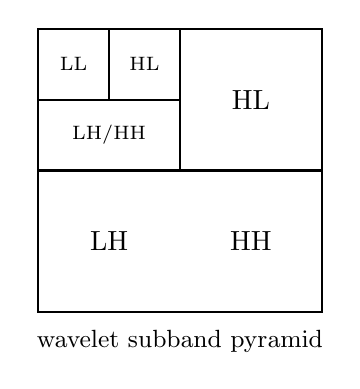
\begin{tikzpicture}[scale=0.9]
\draw[thick] (0,0) rectangle (4,4);
\draw[thick] (0,2) -- (4,2);
\draw[thick] (2,2) -- (2,4);
\draw[thick] (0,3) -- (2,3);
\draw[thick] (1,3) -- (1,4);
\node[font=\scriptsize] at (0.5,3.5) {LL};
\node[font=\scriptsize] at (1.5,3.5) {HL};
\node[font=\scriptsize] at (1,2.5) {LH/HH};
\node at (3,3) {HL}; \node at (1,1) {LH}; \node at (3,1) {HH};
\node[below=1mm, font=\small] at (2,0) {wavelet subband pyramid};
\end{tikzpicture}
\caption{The multiresolution subband layout used by JPEG2000. The top-left corner is a
recursively shrunk low-resolution version of the image (LL); the surrounding bands hold
horizontal (HL), vertical (LH), and diagonal (HH) detail at each scale. Compression keeps
the LL corner with fine precision and quantizes the detail bands, which are mostly zero.}
\label{ch33:fig-subbands}
\end{figure}

JPEG2000 replaces the block DCT with this wavelet transform over the whole image, then
quantizes and entropy-codes the subbands. The payoffs are real: \emph{no blocking}
(there are no blocks), graceful degradation (the same file can be decoded at low or high
resolution by reading fewer or more subbands), and better quality at very high
compression ratios. The costs are also real: it is computationally heavier, more complex
to implement, and -- partly for patent and momentum reasons -- it never displaced plain
JPEG for everyday photos. It found its niche in digital cinema, medical imaging, and
archival, where its quality and scalability justify the cost.

\begin{focusbox}
The main point holds for either transform: \textbf{compression is transform plus
quantization plus entropy coding, and the transform's only job is energy compaction.}
DCT and wavelets are two different bases that both concentrate natural-image energy into
few coefficients; the rest of the pipeline is shared. Choose the basis that compacts your
particular signal best, and the same machinery does the rest.
\end{focusbox}

\section{Code: a DCT-based compressor in a few lines}
\label{ch33:code}

To make it concrete, here is the entire idea -- transform, threshold, inverse -- in a few
lines of NumPy. It is not JPEG (no blocking, no quantization tables, no entropy coder),
but it demonstrates the key step: keep the largest DCT coefficients, zero the
rest, and watch the image survive.

\begin{lstlisting}[language=Python]
import numpy as np
from scipy.fftpack import dctn, idctn   # n-dimensional DCT / IDCT

def compress(img, keep_fraction=0.05):
    """Keep only the largest |DCT| coefficients of a grayscale image."""
    X = dctn(img, norm='ortho')          # 2D DCT of the whole image
    flat = np.sort(np.abs(X), axis=None) # all magnitudes, ascending
    thresh = flat[int((1 - keep_fraction) * flat.size)]
    X_kept = X * (np.abs(X) >= thresh)   # zero out the small coefficients
    recon = idctn(X_kept, norm='ortho')  # inverse DCT -> image back
    nonzero = np.count_nonzero(X_kept)
    print(f"kept {nonzero} of {X.size} coeffs "
          f"({100 * nonzero / X.size:.1f}%)")
    return np.clip(recon, 0, 255)

# Keeping just 5% of coefficients typically yields a clearly
# recognizable image: that 20:1 drop is energy compaction at work.
\end{lstlisting}

\begin{labbox}
Run \texttt{compress} on a photo at \texttt{keep\_fraction} of $0.50, 0.10, 0.05,
0.01$ and look at the results. Around $5\%$ the image is still clearly readable; below
about $1\%$ ringing and smearing take over. Now feed it pure random noise
(\texttt{np.random.rand}) and watch reconstruction quality collapse even at high keep
fractions -- noise does not compact, exactly as the energy argument predicted. Finally,
replace the global DCT with an $8\times 8$ block DCT and a real quantization table, and
you have written the core of JPEG.
\end{labbox}

Figure \ref{ch33:fig-rate} shows the shape you should expect from this experiment:
discarding coefficients costs almost nothing at first, because the ones you drop are tiny,
and only starts to bite once you reach into the coefficients that carry real structure.

\begin{figure}[H]
\centering
\begin{tikzpicture}
\begin{axis}[
  width=12cm, height=5.4cm,
  xlabel={fraction of DCT coefficients kept (largest first)},
  ylabel={reconstruction error},
  xmin=0, xmax=1, ymin=0, ymax=1.05,
  grid=both, grid style={gray!15}, axis lines=box,
  legend pos=north east, legend cell align=left,
  legend style={fill=white, inner sep=4pt, draw=gray!40},
]
\addplot[specred, very thick, domain=0.02:1, samples=80] {exp(-6*x)};
\addlegendentry{natural image (compacts)}
\addplot[gray, dashed, very thick, domain=0:1, samples=2] {1-x};
\addlegendentry{white noise (no compaction)}
\end{axis}
\end{tikzpicture}
\caption{Reconstruction error against the fraction of largest coefficients retained. For a
natural image (red) the error drops fast: keeping a few percent of the coefficients already
captures nearly all the energy. For white noise (gray dashed) every coefficient is equally
important, so error falls only linearly -- you must keep almost everything. This is the
energy-compaction argument turned into a curve.}
\label{ch33:fig-rate}
\end{figure}

\section{Toward the wrist tracker}
\label{ch33:goal}

\begin{goalbox}
Our gesture controller is not going to compress photographs -- but it depends on the
same idea. A wrist-worn IMU streams accelerometer and gyroscope samples at, say,
$200$\,Hz across several axes. Sending every raw sample over Bluetooth Low Energy to a
host, hundreds of times a second, drains the battery and clogs the link. The fix is the
lesson of this chapter applied to a 1D signal: transform a short window, keep the few
coefficients that carry the gesture's energy, and send only those.

In practice we take a window of motion (the swing of a wrist flick, say $128$ samples),
run a DCT or FFT, and find -- just as with images -- that the energy compacts into a
handful of low-frequency coefficients, because deliberate human motion is smooth and
correlated in time, not random. Those few coefficients are simultaneously a
\emph{compressed} representation and an excellent \emph{feature vector} for the classifier
that decides which gesture happened. Transform-domain compaction and transform-domain
feature extraction are the same operation viewed two ways; we will lean on both in
Chapters~38 and~40.

\textbf{A reality checkpoint.} Compacting an IMU window does \emph{not} buy us
information that is not in the signal. A wrist IMU senses the gross motion and orientation
of the forearm; no transform of its data can recover individual finger joint angles,
because that information never reaches the sensor. Continuous finger pose needs sensors on
the fingers (instrumented rings or gloves); finger-level intent without them needs EMG or
force myography on the forearm. The DCT can shrink and sharpen what the IMU measures -- it
cannot conjure what the IMU cannot see.
\end{goalbox}

\section{Transform Coding: Payoffs, Limits, and the Move to Motion Sensors}
\label{ch33:capabilities-limits}

\subsection{What the DCT Enabled}
By compressing continuous-tone photographs by factors of $10\times$ to $30\times$ with minimal perceptible distortion, the 2D Discrete Cosine Transform made three everyday media technologies practical:
\begin{itemize}
  \item \emph{Consumer digital photography:} In the early 1990s, solid-state flash memory cards were measured in single megabytes. Without JPEG, an 8-megabyte CompactFlash card could hold barely two raw uncompressed images; with DCT compression, it held over fifty high-resolution pictures.
  \item \emph{The early World Wide Web:} Dial-up modems operated at 28.8 or 56 kbps. Downloading a single raw 2 MB bitmap took several minutes; a 60 KB JPEG rendered in seconds, which made images a routine part of the web.
  \item \emph{Digital video (MPEG and H.26x):} Video compression adds temporal motion prediction to the spatial 2D DCT. The block DCT became the most heavily executed numerical transform in consumer electronics, powering DVDs, digital television broadcasts, and internet video streaming.
\end{itemize}

\subsection{Limitations}
The block DCT has several limitations:
\begin{itemize}
  \item \emph{Blocking artifacts at high compression:} Because blocks are processed in isolation, boundary pixels across adjacent blocks decouple when quantized heavily, producing harsh checkerboard tiling.
  \item \emph{Ringing and Gibbs oscillations:} Sharp discontinuities (such as black text on a white background, or high-contrast astronomical stars) require an infinite sum of cosines. Truncating high frequencies creates prominent ripples that halo high-contrast edges.
  \item \emph{Rigid stationarity assumption:} Natural images are assumed to be locally stationary Gauss--Markov processes. For non-smooth signals, textures with irregular edges, or pure sensor noise, the DCT provides zero energy compaction.
\end{itemize}

\subsection{From Images to Inertial Sensors}
So far we have treated signals as 1D time series, such as audio, and as 2D pixel grids. In \textbf{Chapter 34} we turn to sensors worn on the body: accelerometers, gyroscopes, and magnetometers that stream 9-axis motion measurements. The same tools, coordinate rotations and transform compaction, will help turn these noisy measurements into real-time gesture recognition for our wearable musical instrument.

\begin{aestheticbox}
JPEG required little new mathematics. Projection
onto an orthonormal basis, Parseval's energy identity, periodic versus symmetric boundary extensions,
the Gibbs phenomenon, and row--column separability all came straight from earlier chapters. The two
new ingredients were \emph{which} basis to project onto (even-symmetric cosines, eliminating block-edge jumps) and \emph{how to spend bits
after transforming} (perceptual quantization followed by entropy coding). Image compression, perceptual audio coding, and compact
sensor features all follow the same pattern: rotate coordinates to concentrate energy, then spend bits on the large coefficients.
\end{aestheticbox}

\section{Summary}
\label{ch33:summary}

\begin{itemize}
\item Compression is a \emph{change of coordinates}: rotate the data into a basis where
energy concentrates into few coefficients, then drop the rest. The transform is lossless;
the loss happens in the rounding afterwards.
\item The \textbf{DCT} is the DFT's real-valued cousin, built by mirroring a block before
going periodic so the seams match. It compacts natural-image energy almost as well as the
optimal but data-dependent KLT, while being a single fixed basis.
\item Energy compaction works because natural images are spatially correlated;
\emph{uncorrelated noise does not compact in any basis} and is therefore incompressible.
\item \textbf{JPEG} = colour transform and chroma subsampling, then per-block $8\times 8$
2D DCT, then perceptual \emph{quantization} (the only lossy transform step), then zigzag,
run-length, and entropy coding. Its artifacts -- blocking, ringing, colour bleed -- come
directly from those choices.
\item \textbf{JPEG2000} swaps the block DCT for a whole-image wavelet transform: no
blocking and resolution scalability, at higher cost and complexity. The pipeline shape --
transform, quantize, entropy-code -- is unchanged.
\item The same transform-and-keep-the-big-coefficients trick compresses and
\emph{features} our IMU gesture windows -- but no transform recovers information the
sensor never captured.
\end{itemize}

\section{Exercises}
\label{ch33:exercises}

\begin{exercise}[Parseval bookkeeping]
\label{ch33:ex-parseval}
A length-$4$ signal has orthonormal-DCT coefficients $X = [10, 4, 0.5, 0.2]$. (a) What is
the total energy $\sum_n x[n]^2$? (b) If you keep only $X[0]$ and $X[1]$ and zero the
rest, what is the energy of the reconstruction error, and what fraction of the total
energy is lost? (c) Comment on why this fraction is so small.
\end{exercise}

\begin{exercise}[Why cosines, not the DFT]
\label{ch33:ex-mirror}
Consider the block $x=[1,2,3,4]$. (a) Sketch the periodic extension the DFT assumes and
mark the jump at the seam. (b) Sketch the even (mirrored) extension the DCT assumes and
confirm there is no jump. (c) In one sentence, explain why the DCT will therefore need
less high-frequency energy to represent this ramp.
\end{exercise}

\begin{exercise}[A 1D DCT by hand]
\label{ch33:ex-dct}
Using \eqref{ch33:dct-1d} with $N=2$ (so $\alpha_0=\sqrt{1/2}$, $\alpha_1=\sqrt{1/2}$ up
to the cosine factor), compute the DCT of $x=[3,5]$. Verify that $X[0]$ is proportional
to the average and that energy is conserved.
\end{exercise}

\begin{exercise}[Quantization arithmetic]
\label{ch33:ex-quant2}
A block has DCT values $X[0,0]=204$, $X[0,1]=23$, $X[1,0]=-9$, and $X[3,3]=14$, with
table entries $Q$ of $16$, $11$, $12$, and $29$ respectively. (a) Compute the quantized
indices $\hat{X}$. (b) Compute the dequantized values $\tilde{X}$ and the error
$X-\tilde{X}$ for each. (c) Which coefficient vanished entirely, and why is that
acceptable?
\end{exercise}

\begin{exercise}[The quality knob]
\label{ch33:ex-quality}
Editors scale the quantization table by a quality factor. Suppose at quality $Q=50$ the
table is the standard one, and at lower quality every entry is multiplied by $3$. (a)
Using $X[2,3]=18$ and base $Q[2,3]=24$, find $\hat{X}$ at quality $50$ and at the lower
quality. (b) Explain in terms of entropy why the lower-quality file is smaller. (c) What
visible artifact grows worst as the table is scaled up?
\end{exercise}

\begin{exercise}[Energy compaction of noise]
\label{ch33:ex-noise}
Argue, using Parseval and the fact that an orthonormal transform of white noise is still
white noise (uncorrelated, equal-variance), that no orthonormal transform can compact the
energy of white noise into fewer coefficients. What does this predict about JPEG's file
size for a photo of television static versus a photo of a clear sky?
\end{exercise}

\begin{exercise}[Zigzag and run-length]
\label{ch33:ex-zigzag}
After quantization, an $8\times 8$ block in zigzag order reads
$[15,\allowbreak -2,\allowbreak 0,\allowbreak 1,\allowbreak 0,\allowbreak 0,\allowbreak 0,\allowbreak 3,\allowbreak 0,\allowbreak\dots,\allowbreak 0]$ (all remaining entries zero). (a) Write
the AC part as (run-of-zeros, value) pairs followed by end-of-block. (b) How many such
symbols are needed, versus $63$ raw AC numbers? (c) Why does the zigzag order, rather
than row-by-row scanning, make these runs longer?
\end{exercise}

\begin{exercise}[Block size trade-off]
\label{ch33:ex-blocksize}
JPEG uses $8\times 8$ blocks. (a) Give one advantage of using larger blocks
($16\times 16$) and one disadvantage. (b) Give one advantage of $4\times 4$ blocks and
one disadvantage. (c) How does the wavelet transform sidestep having to choose a single
block size at all?
\end{exercise}

\begin{exercise}[Separable cost]
\label{ch33:ex-separable}
You must DCT a $512\times 512$ image. (a) Estimate the multiply count for a direct,
non-separable 2D DCT (treat it as a $262144\times 262144$ matrix times a vector). (b)
Estimate it for the separable row-then-column approach using a fast 1D DCT in
$O(N\log N)$. (c) Roughly how many times faster is the separable fast approach?
\end{exercise}

\begin{exercise}[From compression to features (toward the build)]
\label{ch33:ex-features}
You window your wrist IMU's $z$-axis gyro into $128$-sample frames and take a DCT of each
frame. (a) For a smooth, deliberate wrist rotation, predict roughly how many DCT
coefficients carry most of the energy and where they sit. (b) Explain why those same
coefficients make a good fixed-length feature vector for a gesture classifier. (c) State
plainly one thing this DCT feature \emph{cannot} tell you about the hand, and what sensor
you would add to learn it.
\end{exercise}
